% Options for packages loaded elsewhere
\PassOptionsToPackage{unicode}{hyperref}
\PassOptionsToPackage{hyphens}{url}
\PassOptionsToPackage{dvipsnames,svgnames,x11names}{xcolor}
%
\documentclass[
  letterpaper,
  DIV=11,
  numbers=noendperiod,
  oneside]{scrartcl}

\usepackage{amsmath,amssymb}
\usepackage{lmodern}
\usepackage{iftex}
\ifPDFTeX
  \usepackage[T1]{fontenc}
  \usepackage[utf8]{inputenc}
  \usepackage{textcomp} % provide euro and other symbols
\else % if luatex or xetex
  \usepackage{unicode-math}
  \defaultfontfeatures{Scale=MatchLowercase}
  \defaultfontfeatures[\rmfamily]{Ligatures=TeX,Scale=1}
\fi
% Use upquote if available, for straight quotes in verbatim environments
\IfFileExists{upquote.sty}{\usepackage{upquote}}{}
\IfFileExists{microtype.sty}{% use microtype if available
  \usepackage[]{microtype}
  \UseMicrotypeSet[protrusion]{basicmath} % disable protrusion for tt fonts
}{}
\makeatletter
\@ifundefined{KOMAClassName}{% if non-KOMA class
  \IfFileExists{parskip.sty}{%
    \usepackage{parskip}
  }{% else
    \setlength{\parindent}{0pt}
    \setlength{\parskip}{6pt plus 2pt minus 1pt}}
}{% if KOMA class
  \KOMAoptions{parskip=half}}
\makeatother
\usepackage{xcolor}
\usepackage[left=1in,marginparwidth=2.0666666666667in,textwidth=4.1333333333333in,marginparsep=0.3in]{geometry}
\setlength{\emergencystretch}{3em} % prevent overfull lines
\setcounter{secnumdepth}{-\maxdimen} % remove section numbering
% Make \paragraph and \subparagraph free-standing
\ifx\paragraph\undefined\else
  \let\oldparagraph\paragraph
  \renewcommand{\paragraph}[1]{\oldparagraph{#1}\mbox{}}
\fi
\ifx\subparagraph\undefined\else
  \let\oldsubparagraph\subparagraph
  \renewcommand{\subparagraph}[1]{\oldsubparagraph{#1}\mbox{}}
\fi


\providecommand{\tightlist}{%
  \setlength{\itemsep}{0pt}\setlength{\parskip}{0pt}}\usepackage{longtable,booktabs,array}
\usepackage{calc} % for calculating minipage widths
% Correct order of tables after \paragraph or \subparagraph
\usepackage{etoolbox}
\makeatletter
\patchcmd\longtable{\par}{\if@noskipsec\mbox{}\fi\par}{}{}
\makeatother
% Allow footnotes in longtable head/foot
\IfFileExists{footnotehyper.sty}{\usepackage{footnotehyper}}{\usepackage{footnote}}
\makesavenoteenv{longtable}
\usepackage{graphicx}
\makeatletter
\def\maxwidth{\ifdim\Gin@nat@width>\linewidth\linewidth\else\Gin@nat@width\fi}
\def\maxheight{\ifdim\Gin@nat@height>\textheight\textheight\else\Gin@nat@height\fi}
\makeatother
% Scale images if necessary, so that they will not overflow the page
% margins by default, and it is still possible to overwrite the defaults
% using explicit options in \includegraphics[width, height, ...]{}
\setkeys{Gin}{width=\maxwidth,height=\maxheight,keepaspectratio}
% Set default figure placement to htbp
\makeatletter
\def\fps@figure{htbp}
\makeatother

\KOMAoption{captions}{tableheading}
\makeatletter
\makeatother
\makeatletter
\makeatother
\makeatletter
\@ifpackageloaded{caption}{}{\usepackage{caption}}
\AtBeginDocument{%
\ifdefined\contentsname
  \renewcommand*\contentsname{Table of contents}
\else
  \newcommand\contentsname{Table of contents}
\fi
\ifdefined\listfigurename
  \renewcommand*\listfigurename{List of Figures}
\else
  \newcommand\listfigurename{List of Figures}
\fi
\ifdefined\listtablename
  \renewcommand*\listtablename{List of Tables}
\else
  \newcommand\listtablename{List of Tables}
\fi
\ifdefined\figurename
  \renewcommand*\figurename{Figure}
\else
  \newcommand\figurename{Figure}
\fi
\ifdefined\tablename
  \renewcommand*\tablename{Table}
\else
  \newcommand\tablename{Table}
\fi
}
\@ifpackageloaded{float}{}{\usepackage{float}}
\floatstyle{ruled}
\@ifundefined{c@chapter}{\newfloat{codelisting}{h}{lop}}{\newfloat{codelisting}{h}{lop}[chapter]}
\floatname{codelisting}{Listing}
\newcommand*\listoflistings{\listof{codelisting}{List of Listings}}
\makeatother
\makeatletter
\@ifpackageloaded{caption}{}{\usepackage{caption}}
\@ifpackageloaded{subcaption}{}{\usepackage{subcaption}}
\makeatother
\makeatletter
\@ifpackageloaded{tcolorbox}{}{\usepackage[many]{tcolorbox}}
\makeatother
\makeatletter
\@ifundefined{shadecolor}{\definecolor{shadecolor}{rgb}{.97, .97, .97}}
\makeatother
\makeatletter
\@ifpackageloaded{sidenotes}{}{\usepackage{sidenotes}}
\@ifpackageloaded{marginnote}{}{\usepackage{marginnote}}
\makeatother
\makeatletter
\makeatother
\ifLuaTeX
  \usepackage{selnolig}  % disable illegal ligatures
\fi
\IfFileExists{bookmark.sty}{\usepackage{bookmark}}{\usepackage{hyperref}}
\IfFileExists{xurl.sty}{\usepackage{xurl}}{} % add URL line breaks if available
\urlstyle{same} % disable monospaced font for URLs
\hypersetup{
  pdftitle={Take Home Exercise 01},
  pdfauthor={Huo Da},
  colorlinks=true,
  linkcolor={blue},
  filecolor={Maroon},
  citecolor={Blue},
  urlcolor={Blue},
  pdfcreator={LaTeX via pandoc}}

\title{Take Home Exercise 01}
\author{Huo Da}
\date{}

\begin{document}
\maketitle
\ifdefined\Shaded\renewenvironment{Shaded}{\begin{tcolorbox}[boxrule=0pt, breakable, borderline west={3pt}{0pt}{shadecolor}, interior hidden, enhanced, sharp corners, frame hidden]}{\end{tcolorbox}}\fi

\hypertarget{overview-of-task}{%
\section{1. Overview of Task}\label{overview-of-task}}

Age-sex pyramid is an analytical visualisation commonly used by
demographers to reveal the structure of population by gender and age
group. In this take-home exercise, you are required to reveal the
demographic structure of Singapore at planning area level by using
age-sex pyramid method. Instead of plotting a single age-sex pyramid,
however, you are required to display nine selected planning areas on a
single view by using trellis display (also know as small-multiple plot).

Singapore Residents by Planning Area / Subzone, Age Group, Sex and Type
of Dwelling, June 2022 should be used to prepare the analytical
visualisation. The data can be downloaded
\href{https://www.singstat.gov.sg/find-data/search-by-theme/population/geographic-distribution/latest-data}{here}.

\hypertarget{visualisation}{%
\section{2. Visualisation}\label{visualisation}}

The proposed visualisation can be viewed on Tableau Public
\href{https://public.tableau.com/app/profile/huoda1027/viz/TakeHome_Ex01_16742612602400/Dashboard1?publish=yes}{here}.

\begin{figure*}

{\centering 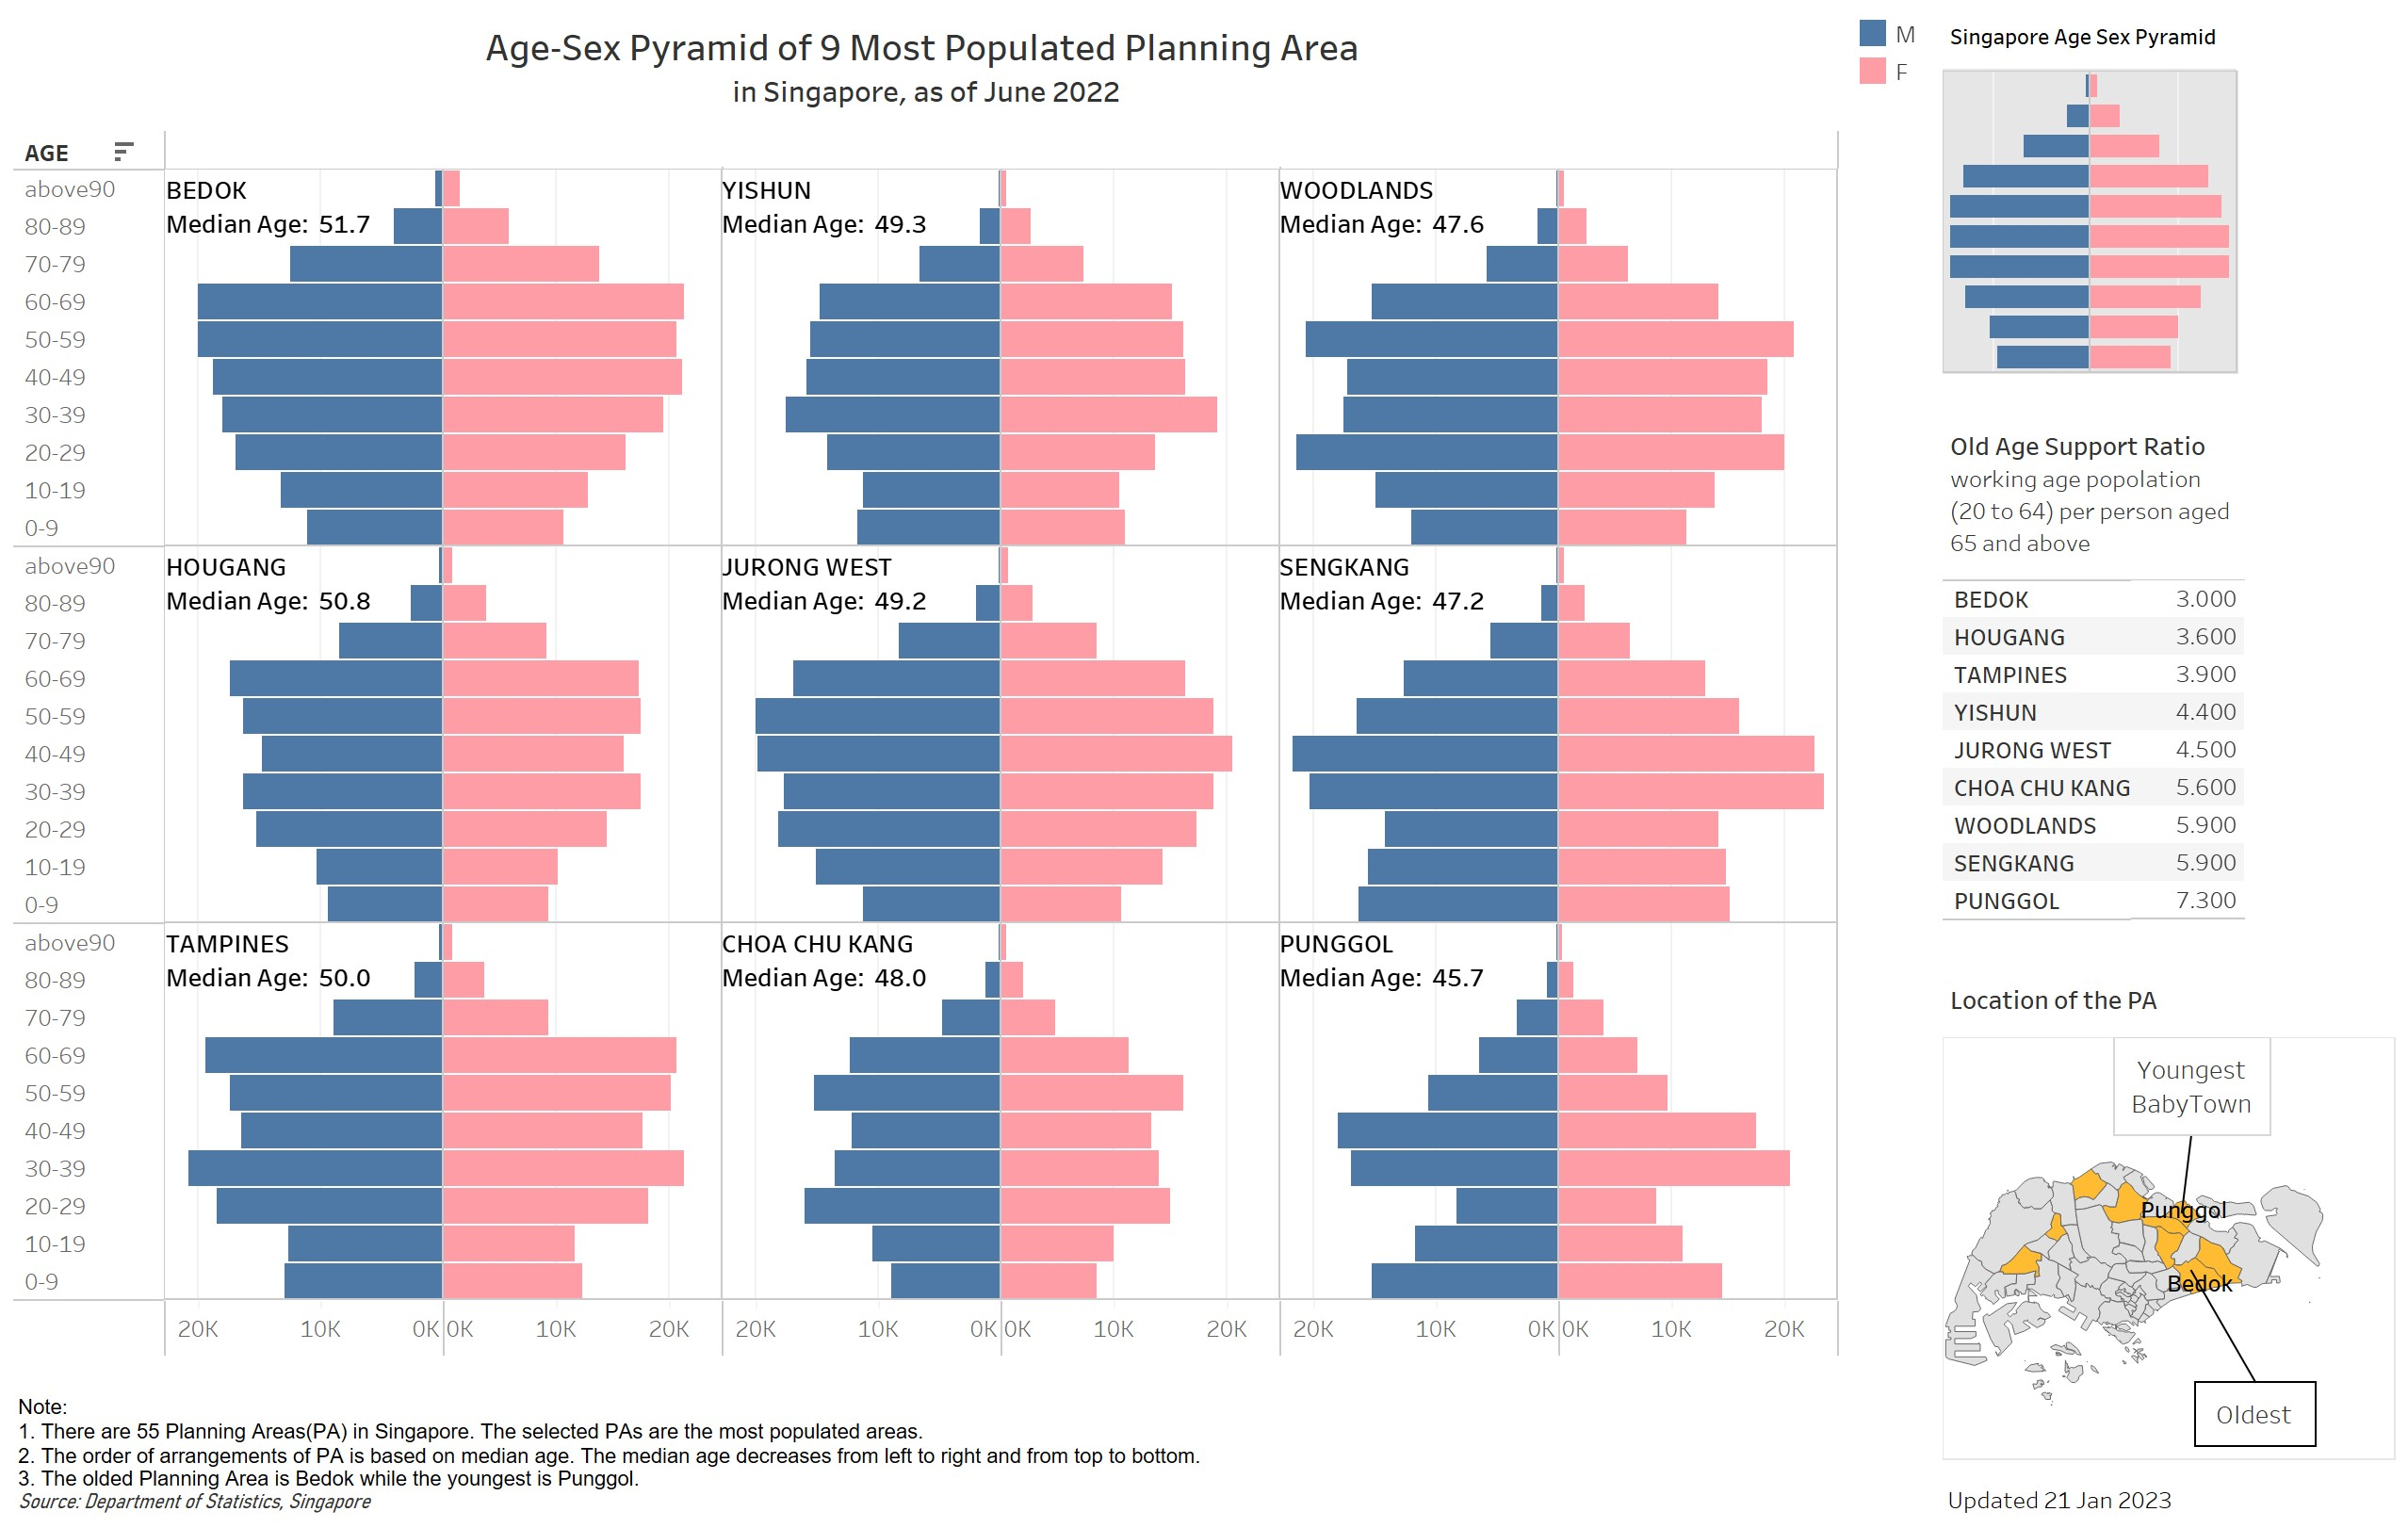
\includegraphics{images/vis-02.jpg}

}

\end{figure*}

\hypertarget{key-observations}{%
\section{3. Key Observations}\label{key-observations}}

\begin{itemize}
\tightlist
\item
  \textbf{Median Age}
\end{itemize}

On the top-left corner of each pyramid, the name of the planning
area(PA) and median age of the respective PA are shown. For example,
Bedok has the highest median age of 52, while Punggol has the lowest
median age of 45.7. The population in Punggol is much younger than those
in Bedok.

\begin{marginfigure}

{\centering 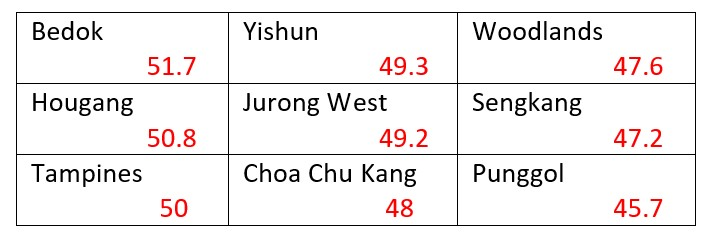
\includegraphics[width=7.21875in,height=\textheight]{images/median age.jpg}

}

\end{marginfigure}

Note that We have arranged that the pyramids for each PA. The order is
based on median age. The median age decreases from left to right and
from top to bottom.

\begin{itemize}
\tightlist
\item
  \textbf{Age Structure}
\end{itemize}

In Bedok and in Hougang (top left corner), each consecutive age group
moving up the pyramids gets broader from 0 to 69 years old and then gets
narrower from 70 years old. This is a typical aging population. The
population pyramid of Singapore shown on the right margin also has the
same structure. The aging population mainly due to factors such as low
fertility rate and high life expectancy.

In Punggol and SengKang (bottom right corner), there are bulges in the
age groups of 0 - 10 and 30 to 49. We can conclude that many of the
residents living in these PA are young families with children. According
to Straits Time, Punggol was dubbed as Singapore's baby town in 2017.

The pyramids in other PAs have narrow base which represents a low birth
rate. The population is mostly clustered around the age groups of 20 to
40 and 50 to 70. While in the younger PA such as Woodland, the peaks are
at 20 to 29 and 50 to 59.

While in elderly PA such as Tampines, the peaks are at 30 to 39 and 60
to 69. On average, the population in Woodlands is 2.4 yrs younger than
those in Tampines.

Overall, the pyramid in the two oldest PA has a similar shape as
Singapore, while the pyramid in the two youngest PA has a very different
shape as Singapore.

\begin{itemize}
\tightlist
\item
  \textbf{Old Age Support Ratio}
\end{itemize}

According to Singapore Department of Statistics, the old age support
ratio represents the number of people who are capable of providing
economic support (20 to 64) to the number of older people who may be
dependent on others support (65 and above). The value of old age support
ratio for each PA is as shown on the right margin. Not surprisingly, the
value of this ration increases from the elder PA to the younger PA. One
elderly people aged 65 and above is supported by 3 younger people in
Bedok, and is supported by 7.3 younger people in Punggol.

\begin{marginfigure}

{\centering 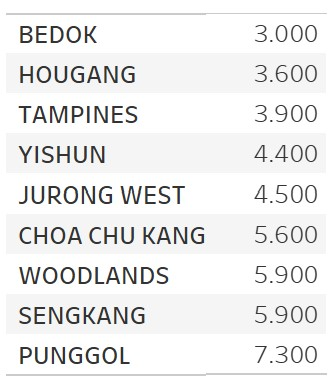
\includegraphics{images/old age support ratio-02.jpg}

}

\end{marginfigure}

The order of PA in the table is arranged according to median age in
descending order, i.e.~from the greatest to the smallest. We noticed
that the value of the old support ratio is almost in ascending order,
expect the woodlands and Sengkang has equal value.

\begin{itemize}
\tightlist
\item
  \textbf{Males vs.~Females}
\end{itemize}

In all pyramids, there is no symmetry between males and females in older
age groups (\textgreater70 yrs). The women are living longer than men.
There are also slightly more males than females in younger age groups,
as the natural sex ratio at birth is around 105 boys per 100 girls. The
ratio is not skewed than would occur naturally.

\begin{itemize}
\tightlist
\item
  \textbf{Location of 9 selected Planning Areas}
\end{itemize}

There are 7 out of 9 most populated PAs in the East and North of
Singapore. The youngest PA is located in the north of Singapore and the
oldest PA is located in the east of Singapore.

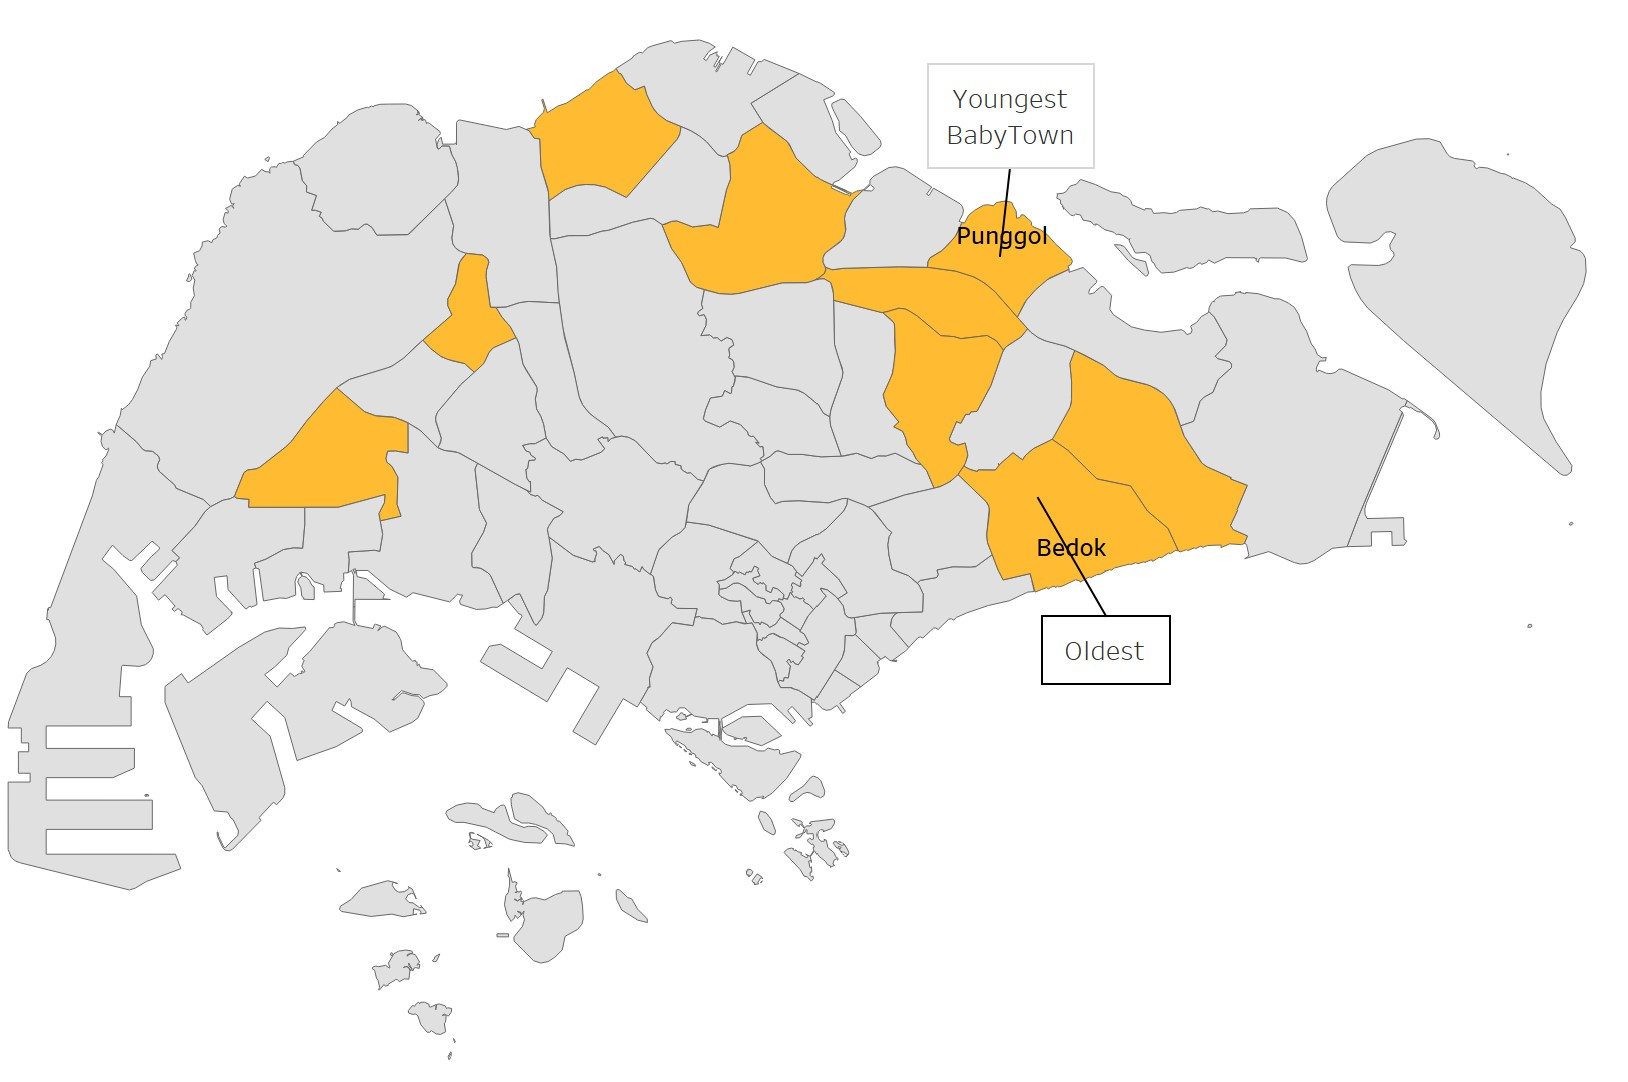
\includegraphics{images/location of PA-02.jpg}

\hypertarget{step-by-step-preparation}{%
\section{4. Step by Step Preparation}\label{step-by-step-preparation}}

This section details the steps required to produce the dashboard as
described in section 2.

\hypertarget{use-tableau-prep-for-data-preparation}{%
\subsection{4.1 Use Tableau Prep for data
preparation}\label{use-tableau-prep-for-data-preparation}}

The flow of the data preparation to obtain the Median Age and Old Age
Support Ratio for each PA is as shown below.

\begin{figure}

{\centering 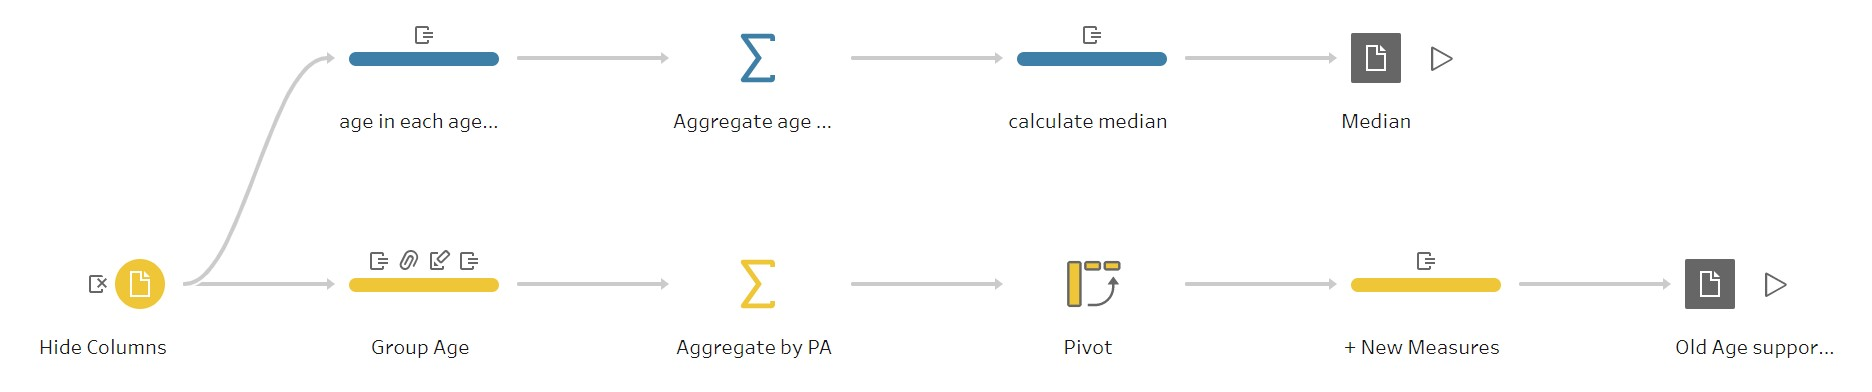
\includegraphics{images/flow-01.jpg}

}

\caption{Fig 4.1.1 Tableau Prep Workflow}

\end{figure}

\begin{figure*}

\begin{longtable}[]{@{}
  >{\raggedright\arraybackslash}p{(\columnwidth - 4\tabcolsep) * \real{0.1000}}
  >{\raggedright\arraybackslash}p{(\columnwidth - 4\tabcolsep) * \real{0.3000}}
  >{\raggedright\arraybackslash}p{(\columnwidth - 4\tabcolsep) * \real{0.6000}}@{}}
\toprule()
\begin{minipage}[b]{\linewidth}\raggedright
No.
\end{minipage} & \begin{minipage}[b]{\linewidth}\raggedright
Step
\end{minipage} & \begin{minipage}[b]{\linewidth}\raggedright
Screenshot
\end{minipage} \\
\midrule()
\endhead
1 & Load the originl data csv into Tableau Prep by click the plus symbol
besides Connections, then choose Text File. &
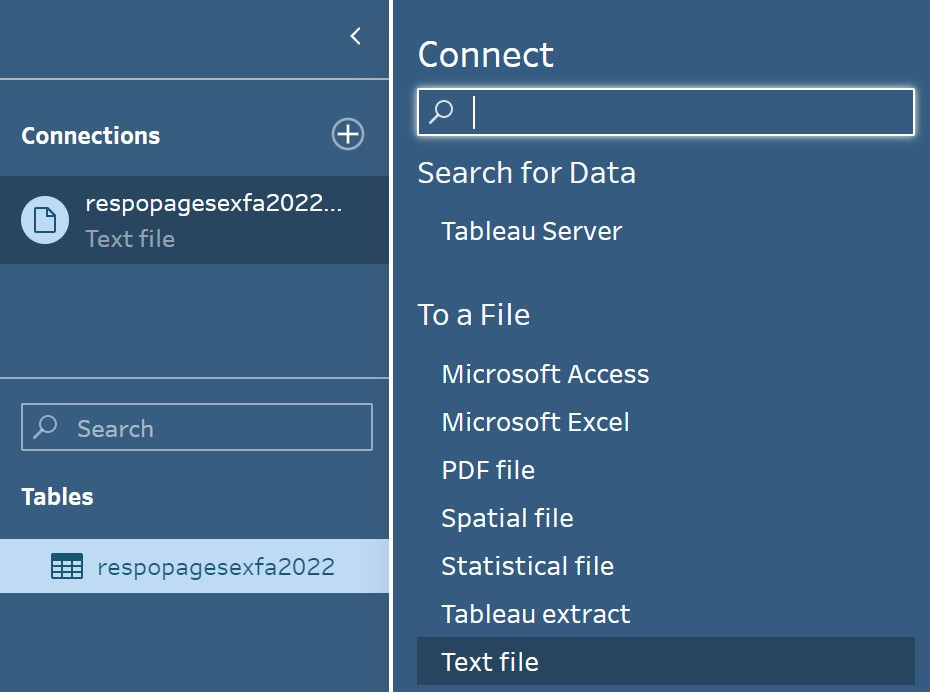
\includegraphics{images/1.jpg} \\
2 & Hide unnecessary columns by unclick the specific Field Name. In this
task, the SZ(subzone), FA(floor area), Time(2022) are hided. &
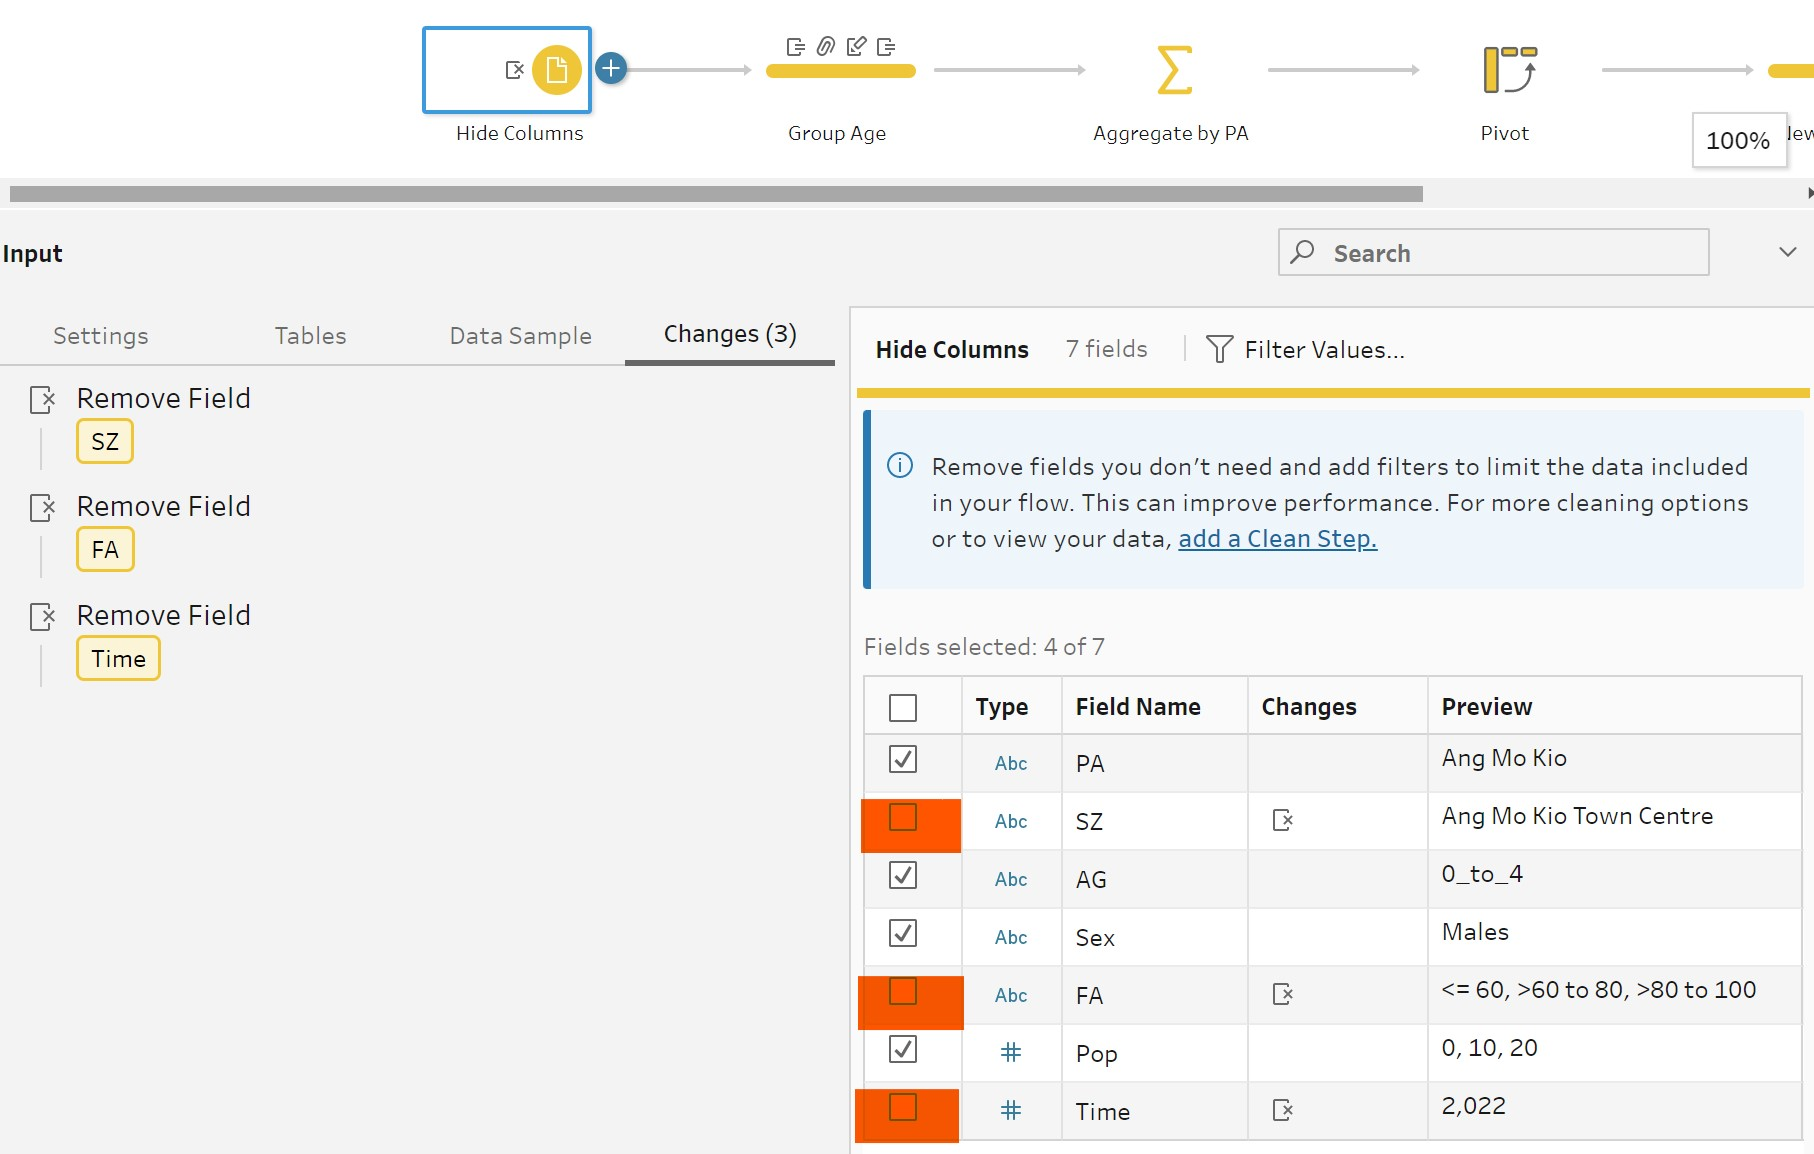
\includegraphics{images/2.jpg} \\
3 & Calculate median age for each age group, and the total age for each
row = median age * population in each row. &
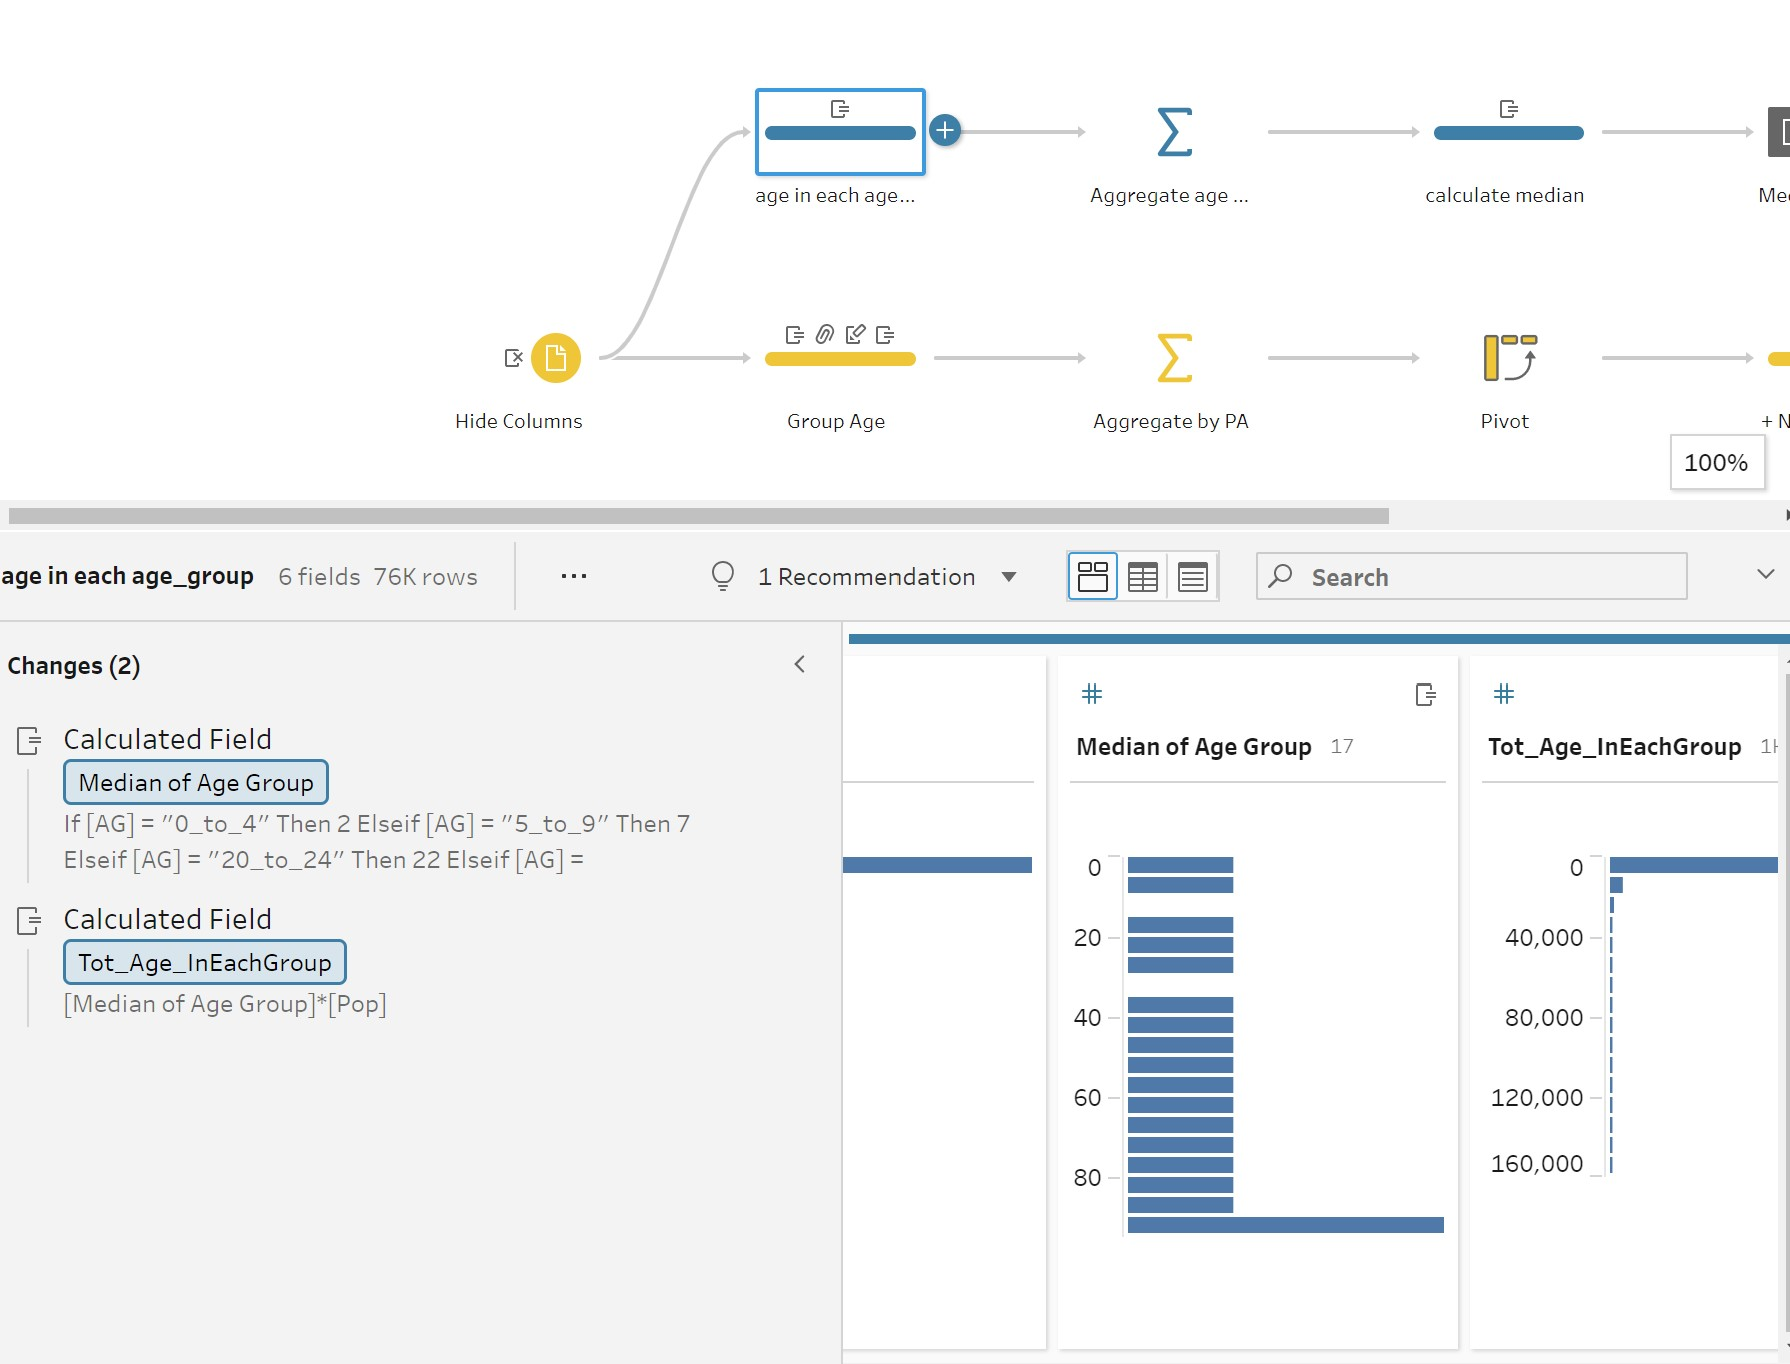
\includegraphics{images/3.jpg} \\
4 & Aggregate the age and population for each PA. &
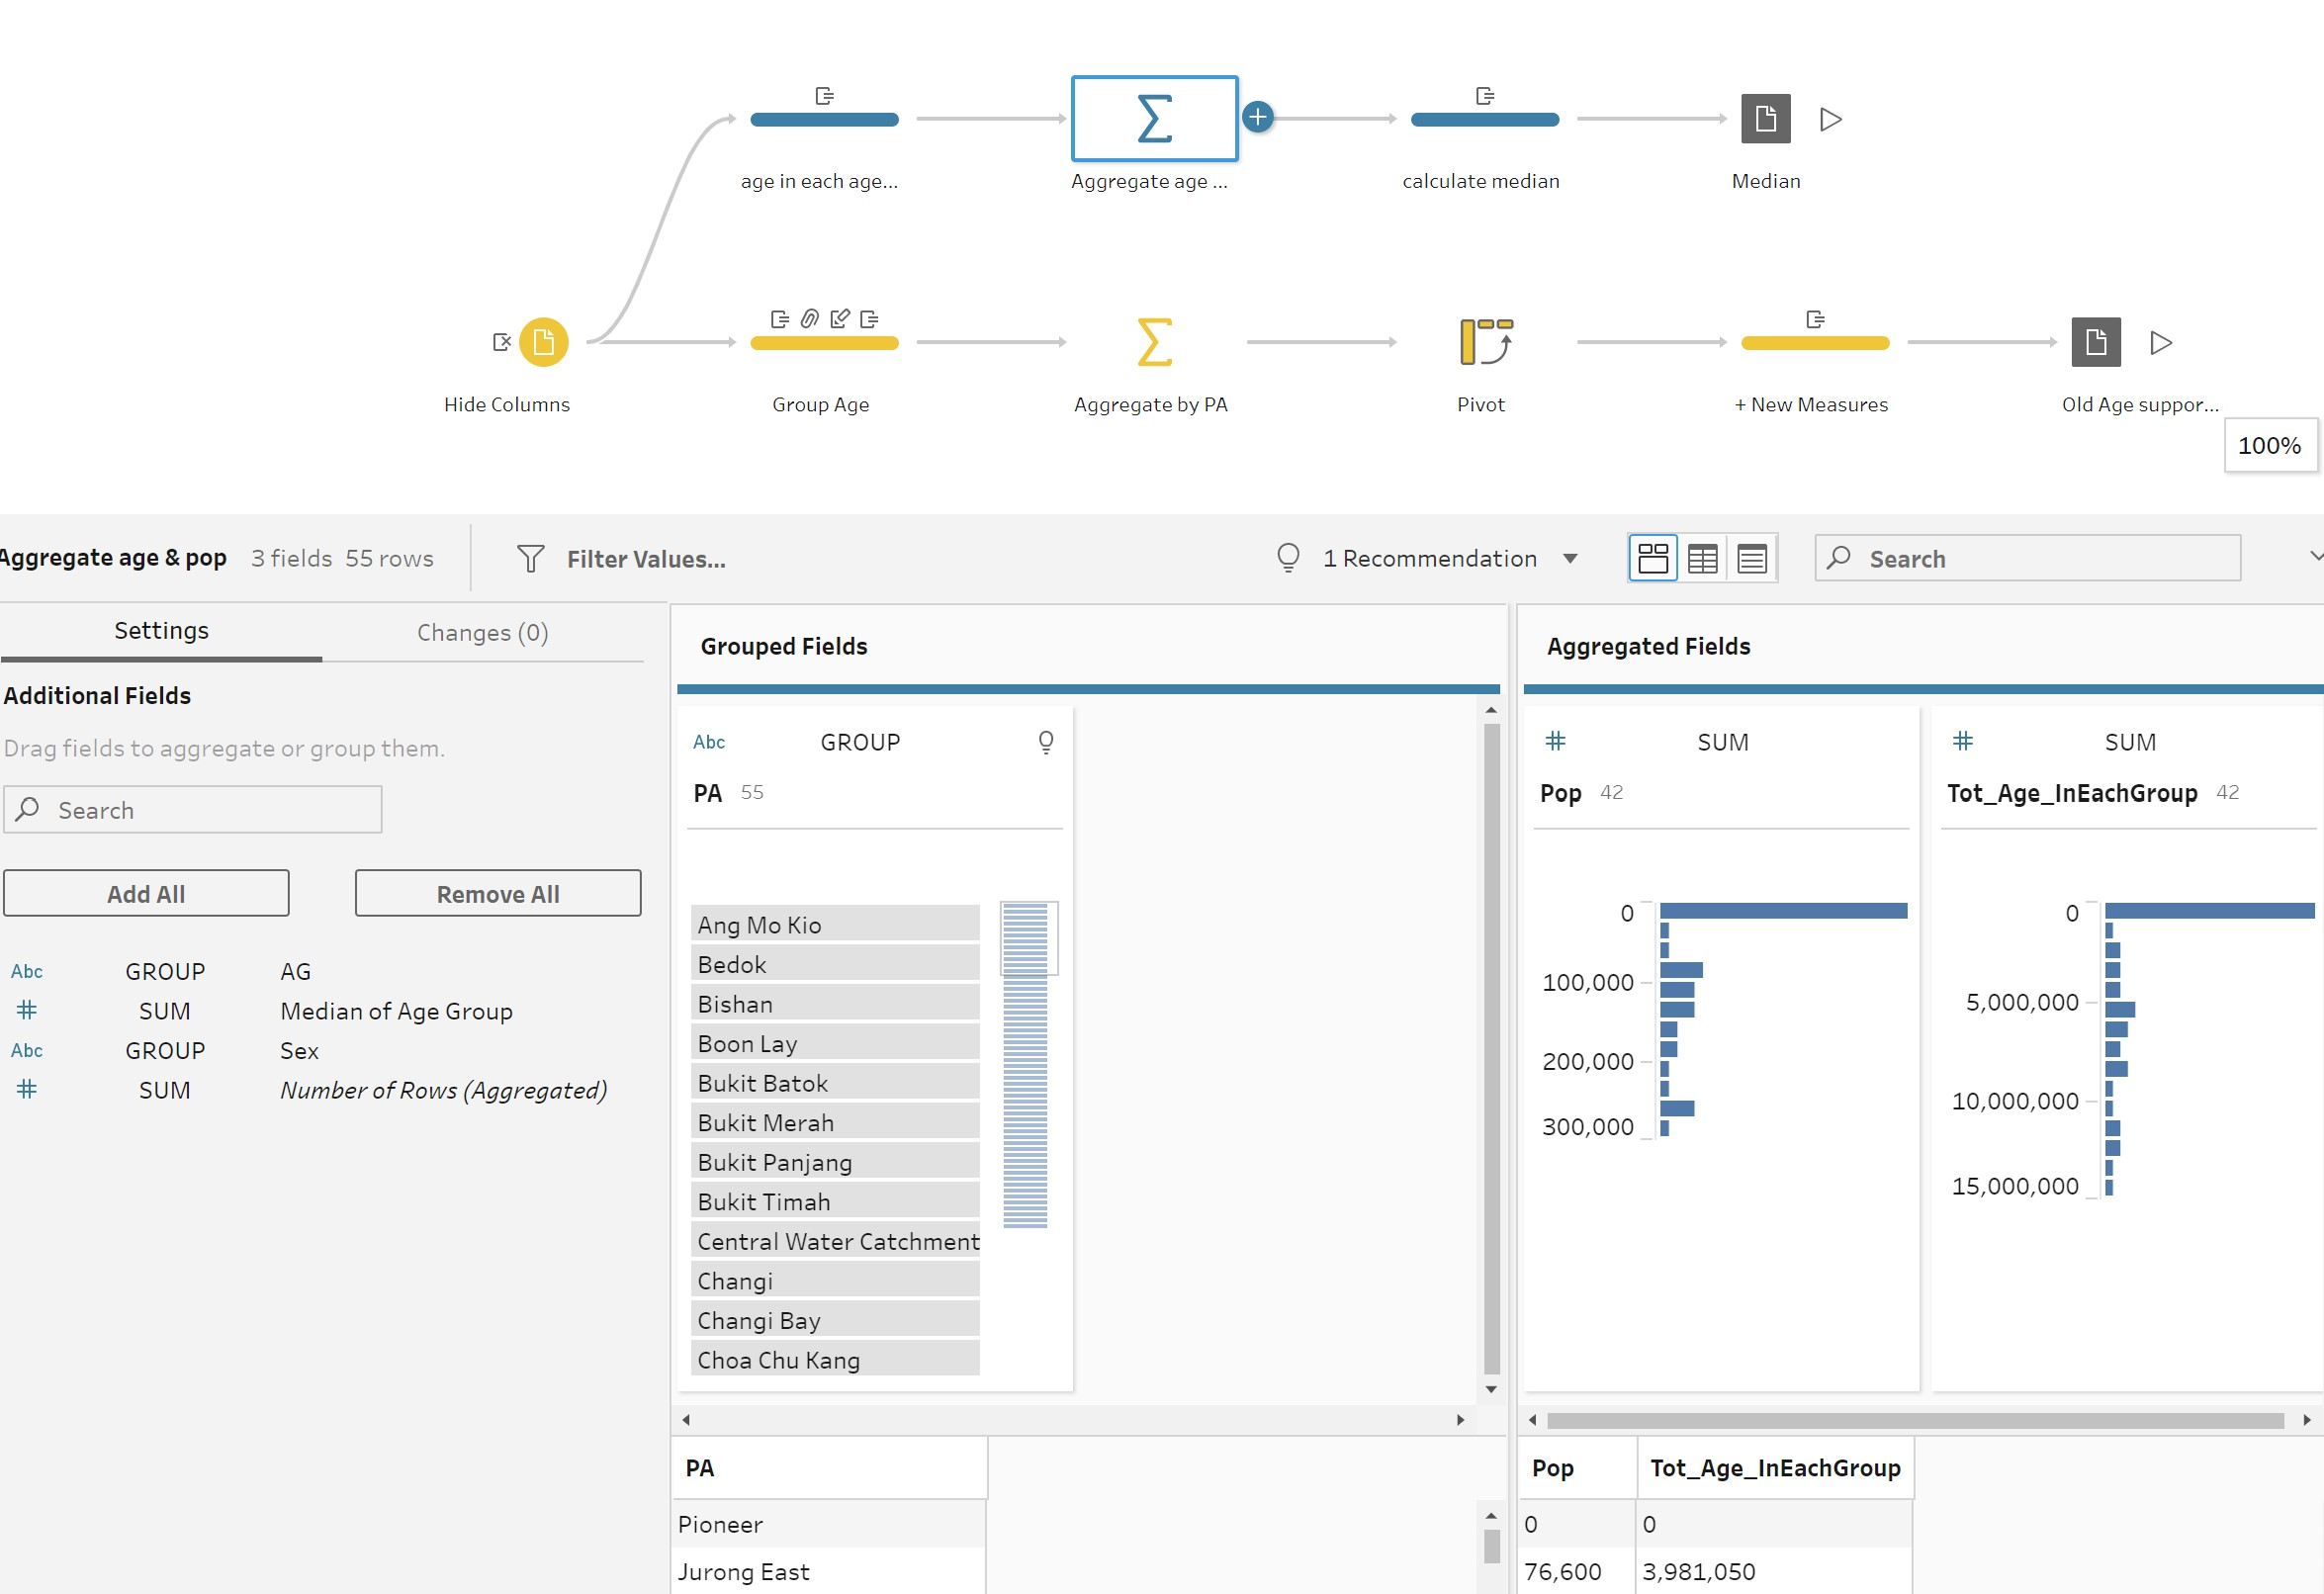
\includegraphics{images/4.jpg} \\
5 & Calculate the median age for each PA and output as csv file. &
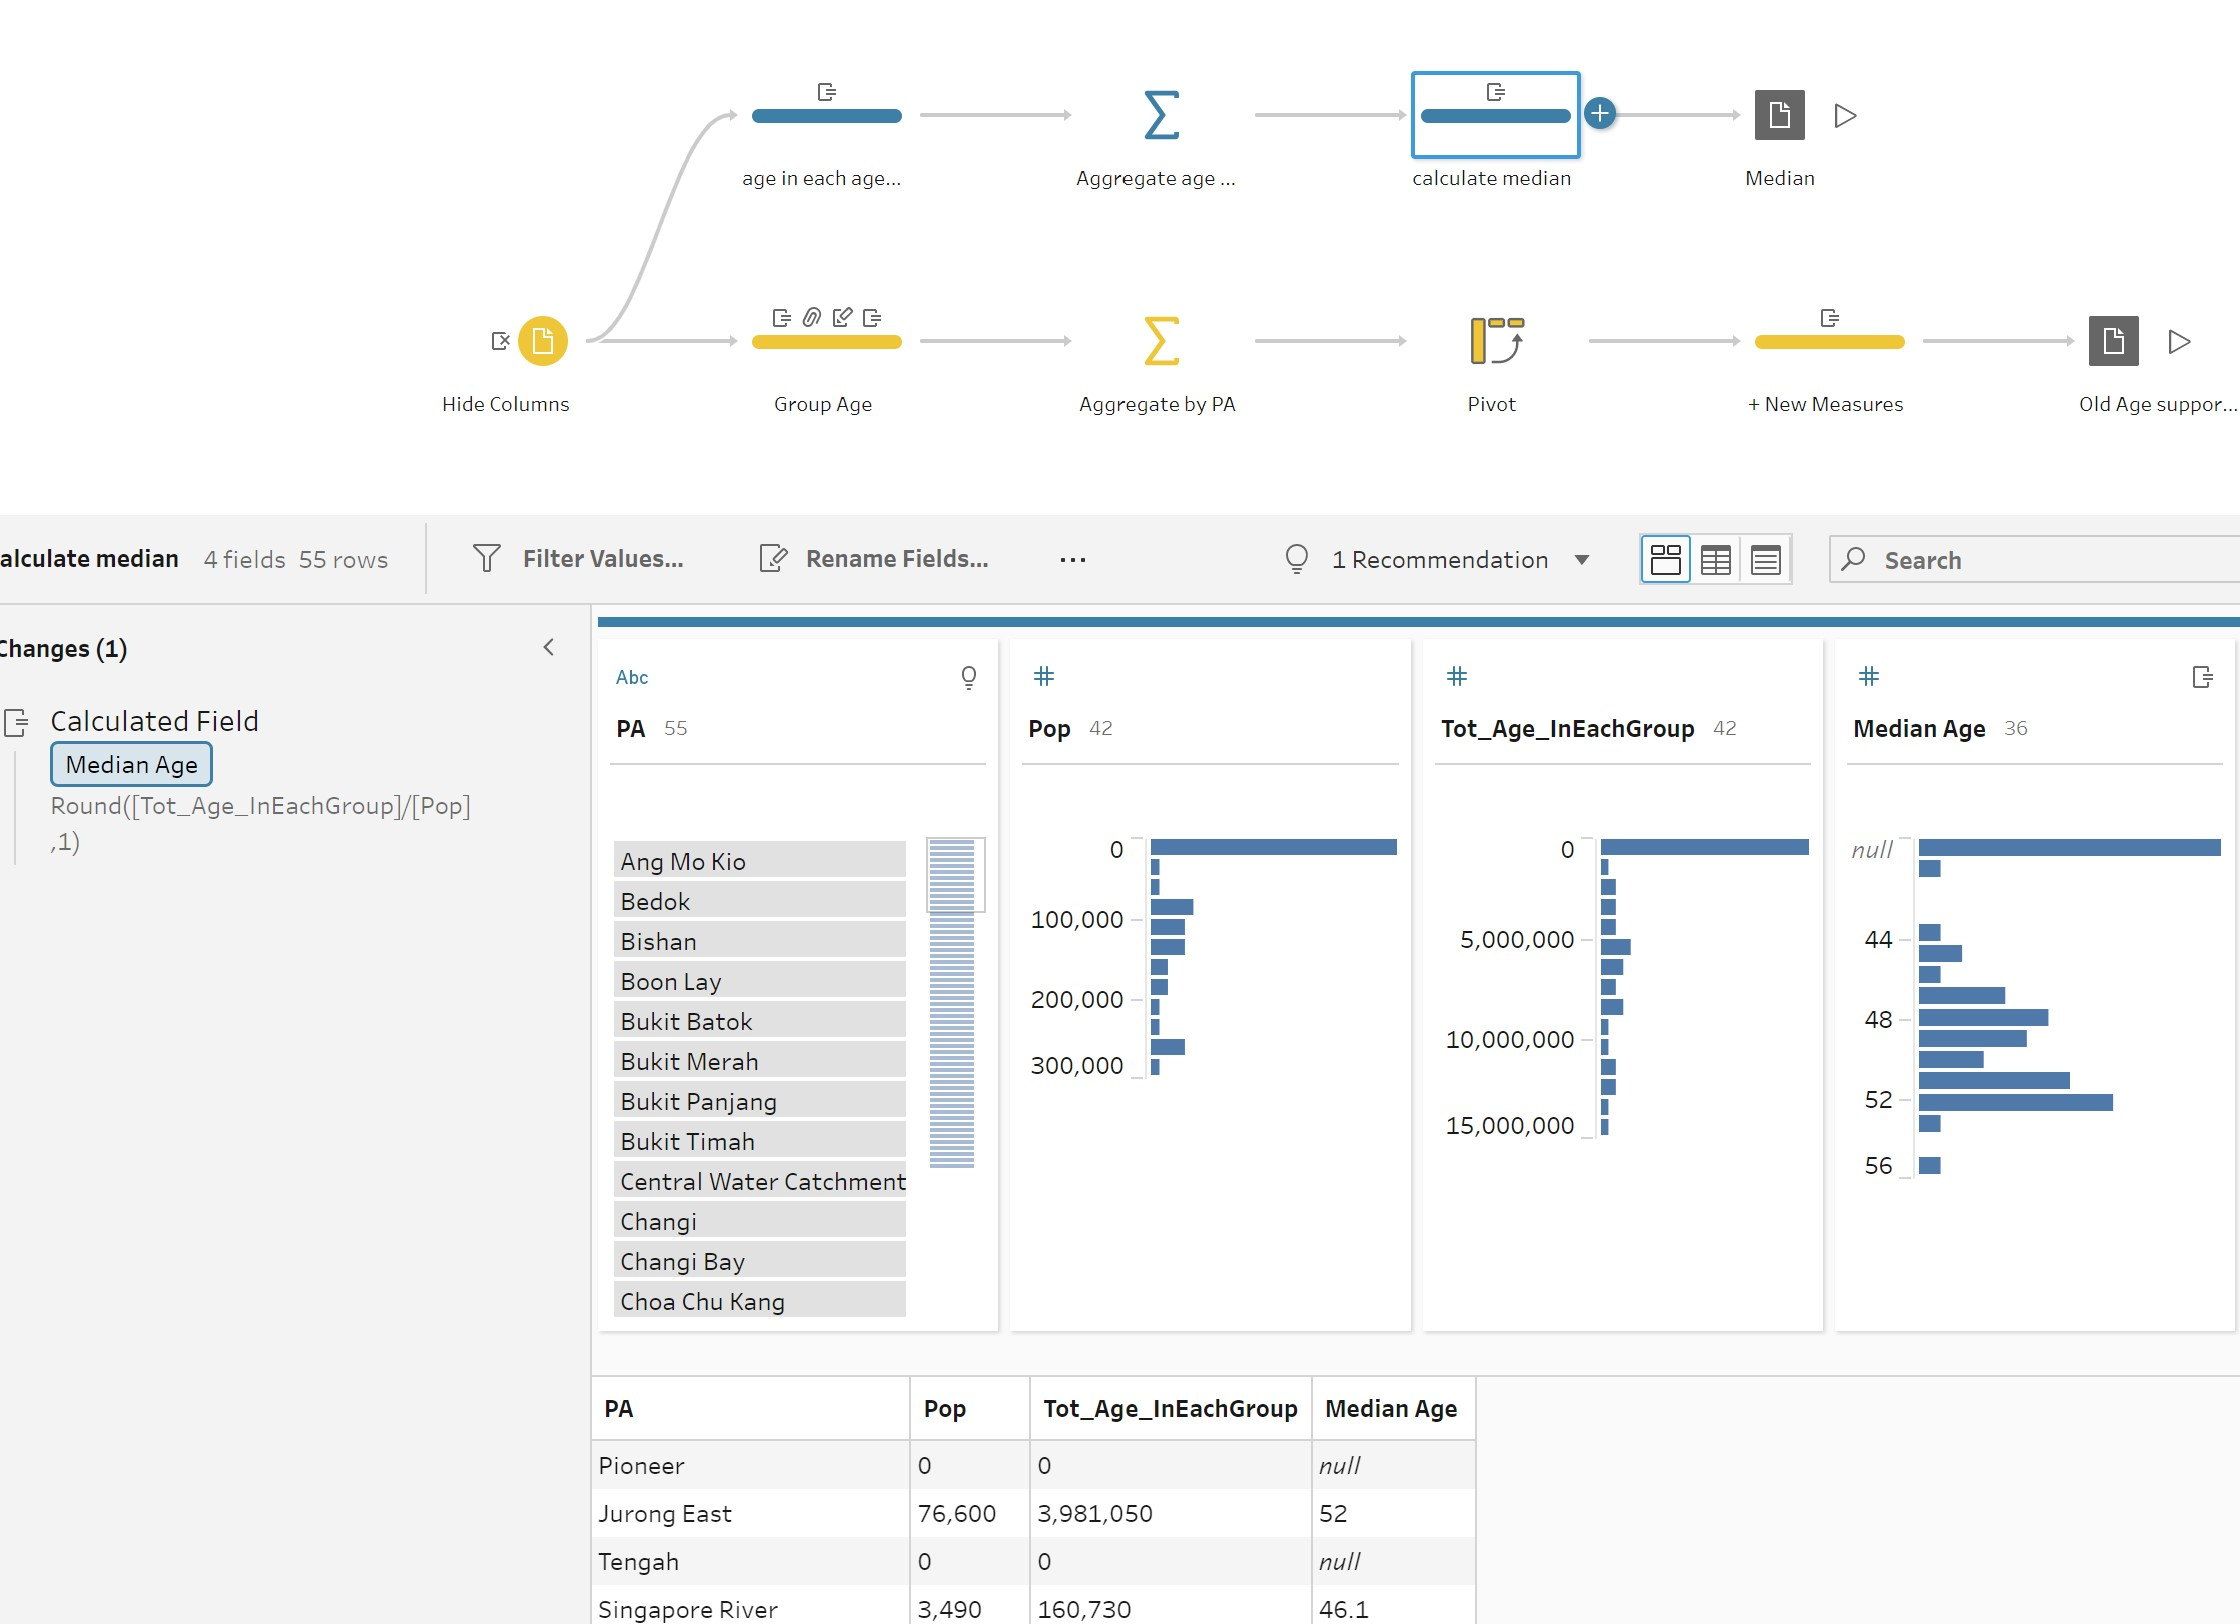
\includegraphics{images/5.jpg} \\
6 & Create new age group by grouping original age groups. &
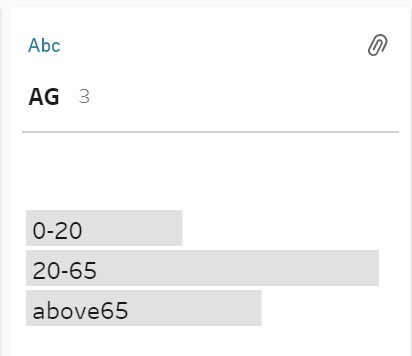
\includegraphics{images/6.jpg} \\
7 & Aggregate population for each PA. &
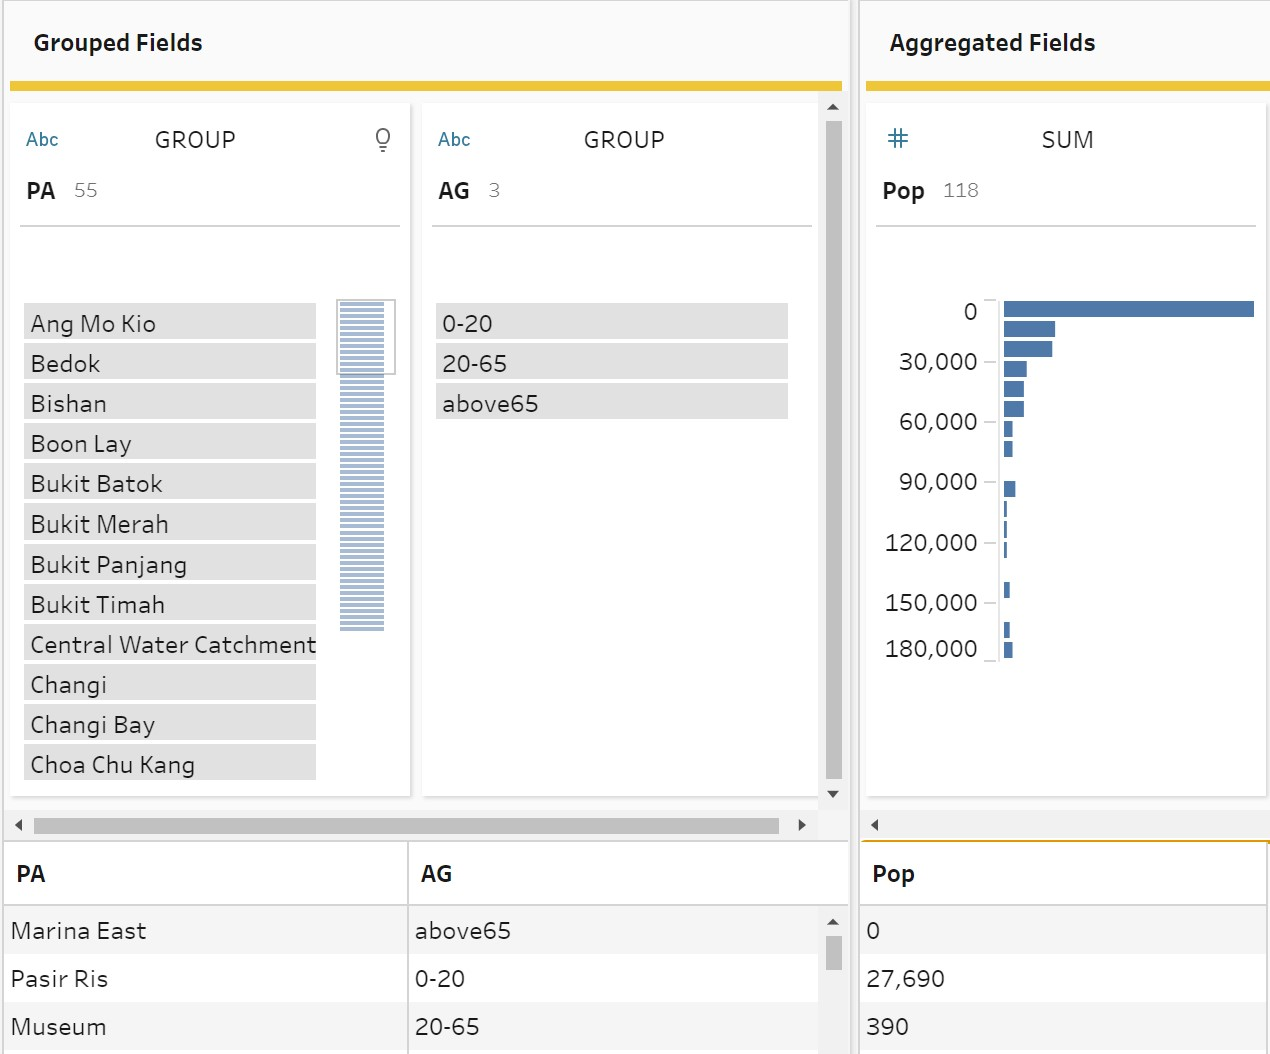
\includegraphics{images/7.jpg} \\
8 & Convert the long table to wide table. &
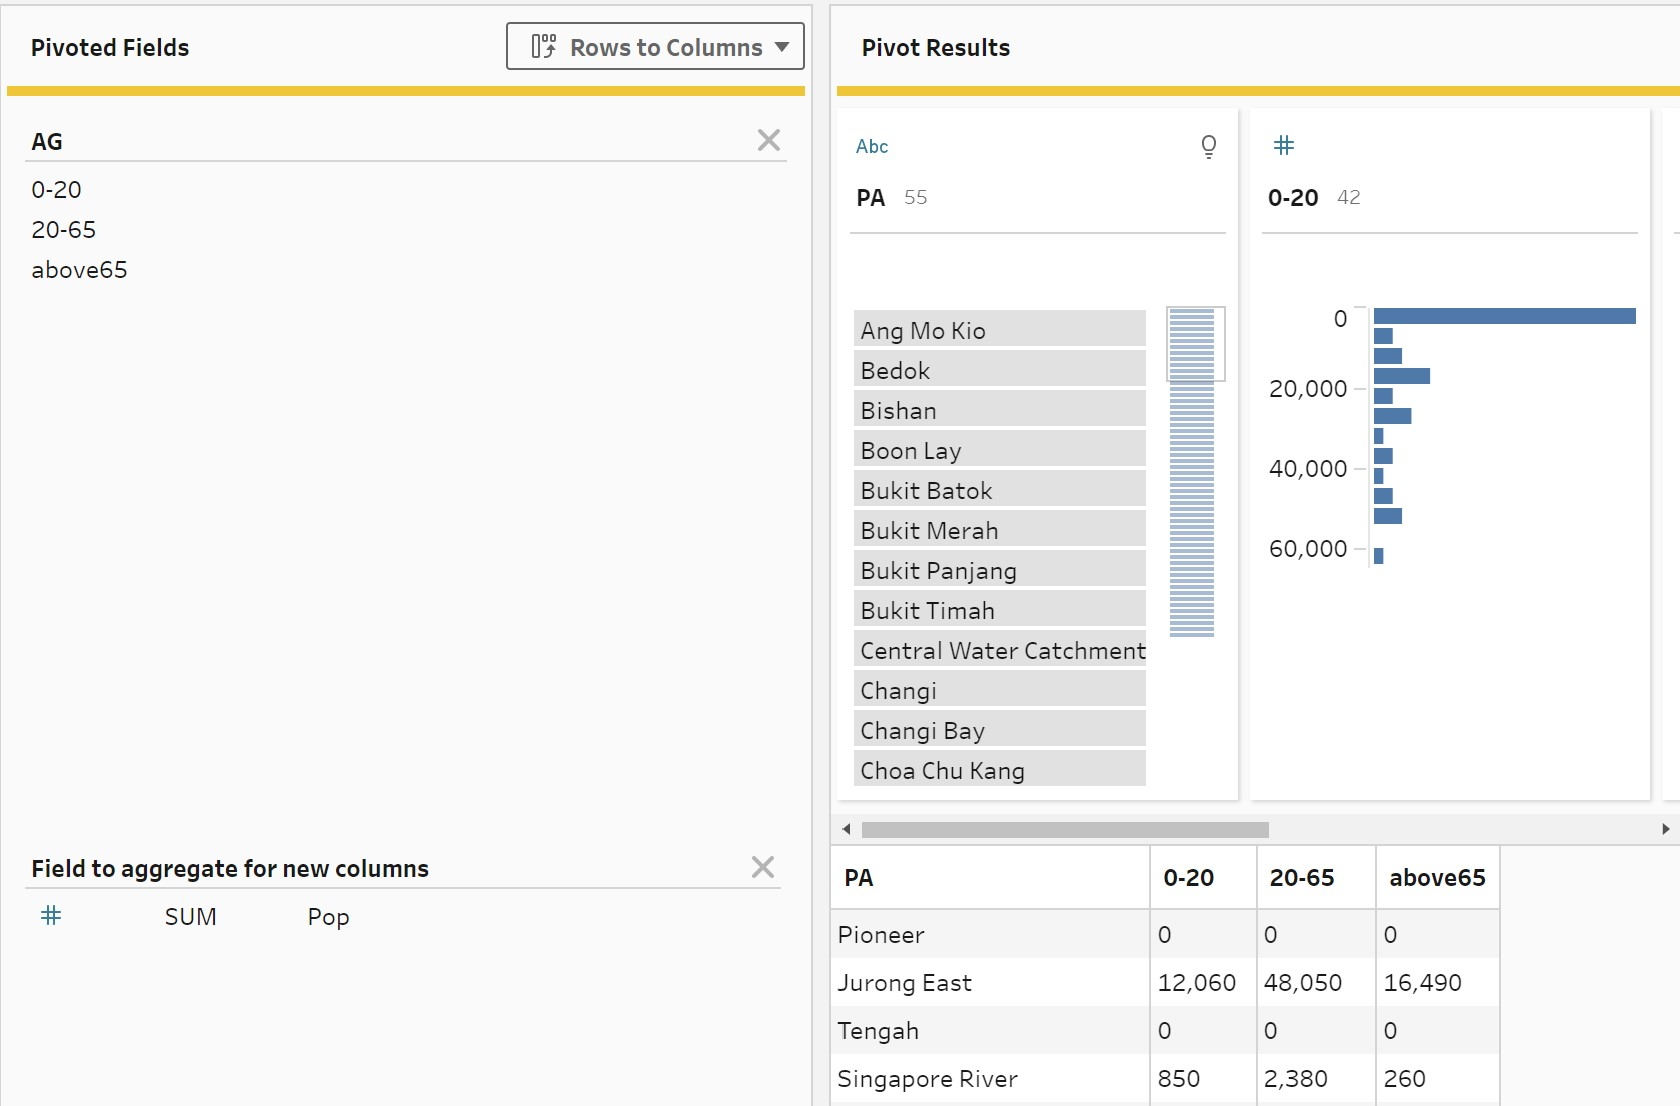
\includegraphics{images/8.jpg} \\
9 & Calculate old age support ratio for each PA and output as csv file.
& 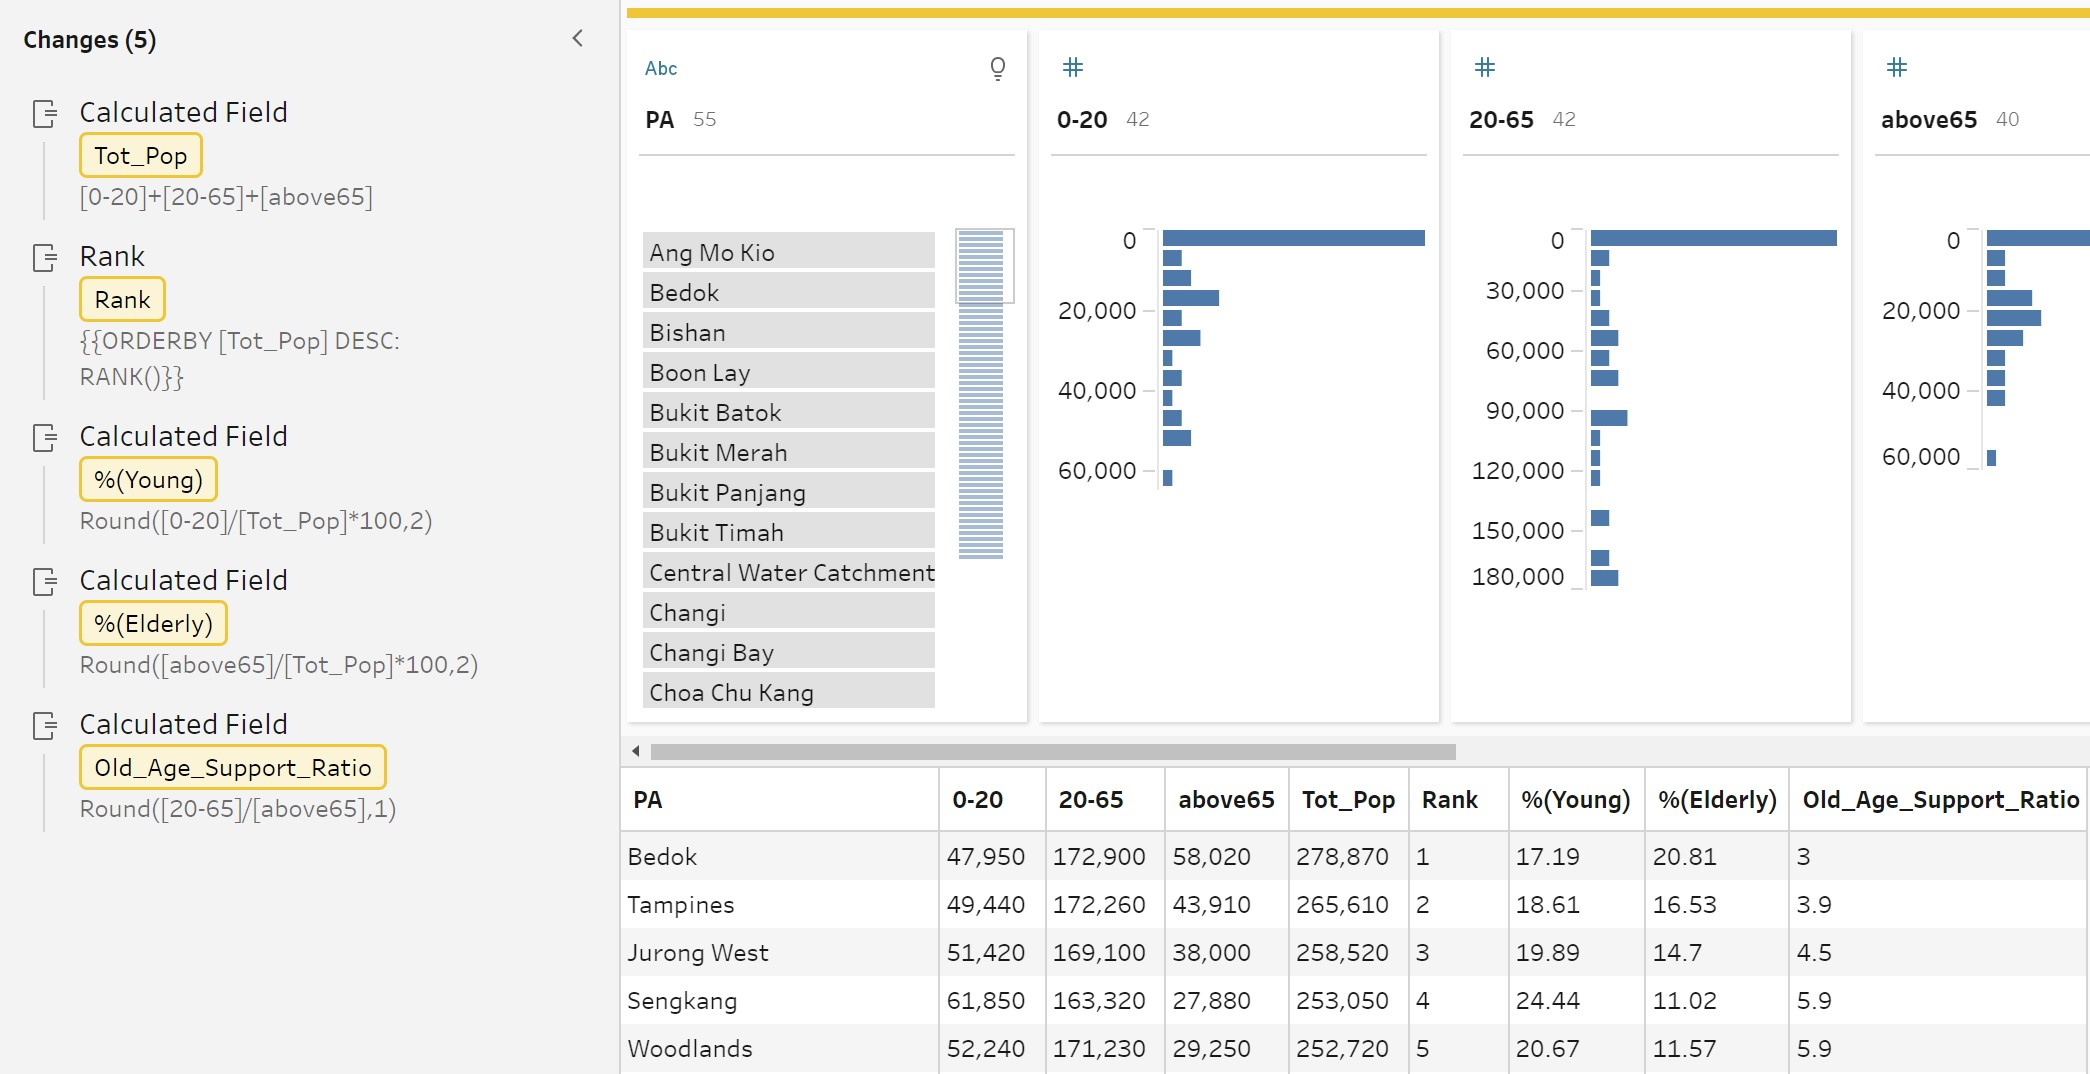
\includegraphics{images/9.jpg} \\
\bottomrule()
\end{longtable}

\end{figure*}

\hypertarget{build-dashboard}{%
\subsection{4.2 Build Dashboard}\label{build-dashboard}}

\hypertarget{draw-map-highlighting-the-9-most-populated-pa-in-singapore}{%
\subsubsection{4.2.1 Draw Map Highlighting the 9 Most Populated PA in
Singapore}\label{draw-map-highlighting-the-9-most-populated-pa-in-singapore}}

\begin{figure*}

\begin{longtable}[]{@{}
  >{\raggedright\arraybackslash}p{(\columnwidth - 4\tabcolsep) * \real{0.1000}}
  >{\raggedright\arraybackslash}p{(\columnwidth - 4\tabcolsep) * \real{0.3000}}
  >{\raggedright\arraybackslash}p{(\columnwidth - 4\tabcolsep) * \real{0.6000}}@{}}
\toprule()
\begin{minipage}[b]{\linewidth}\raggedright
No.
\end{minipage} & \begin{minipage}[b]{\linewidth}\raggedright
Step
\end{minipage} & \begin{minipage}[b]{\linewidth}\raggedright
Screenshot
\end{minipage} \\
\midrule()
\endhead
1 & Load the original population .csv file, subzone by planning area
.shp file and the two output files with derived measures (old age
support ratio and median age) in each planning region .csv files in
Tableau Desktop( for mapping purpose). & \\
2 & Drag all the files besides the original of population file to join
files by matching PA (the name of the planning areas). Note that in .shp
file, the name of planning areas are in upper case. We need to edit the
matching by Upper(PA) = PA(.shp file). &
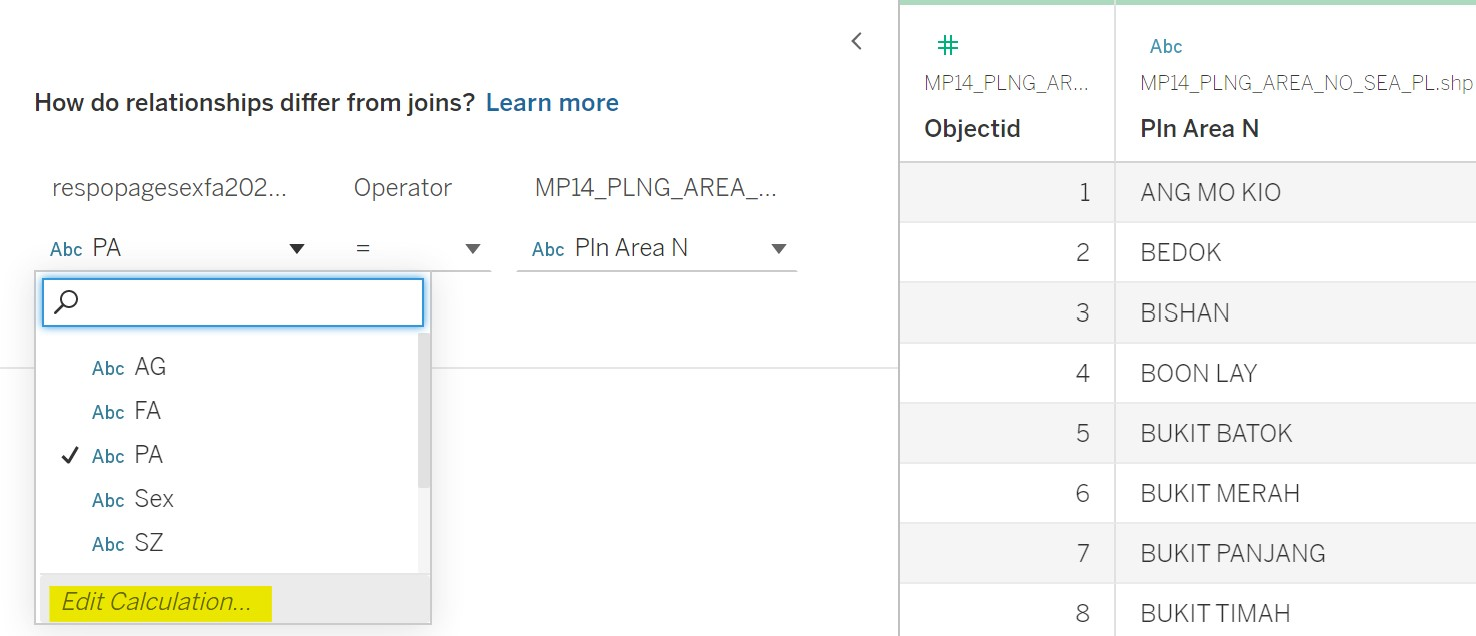
\includegraphics{images/join.jpg} \\
3 & Files are joined successfully. &
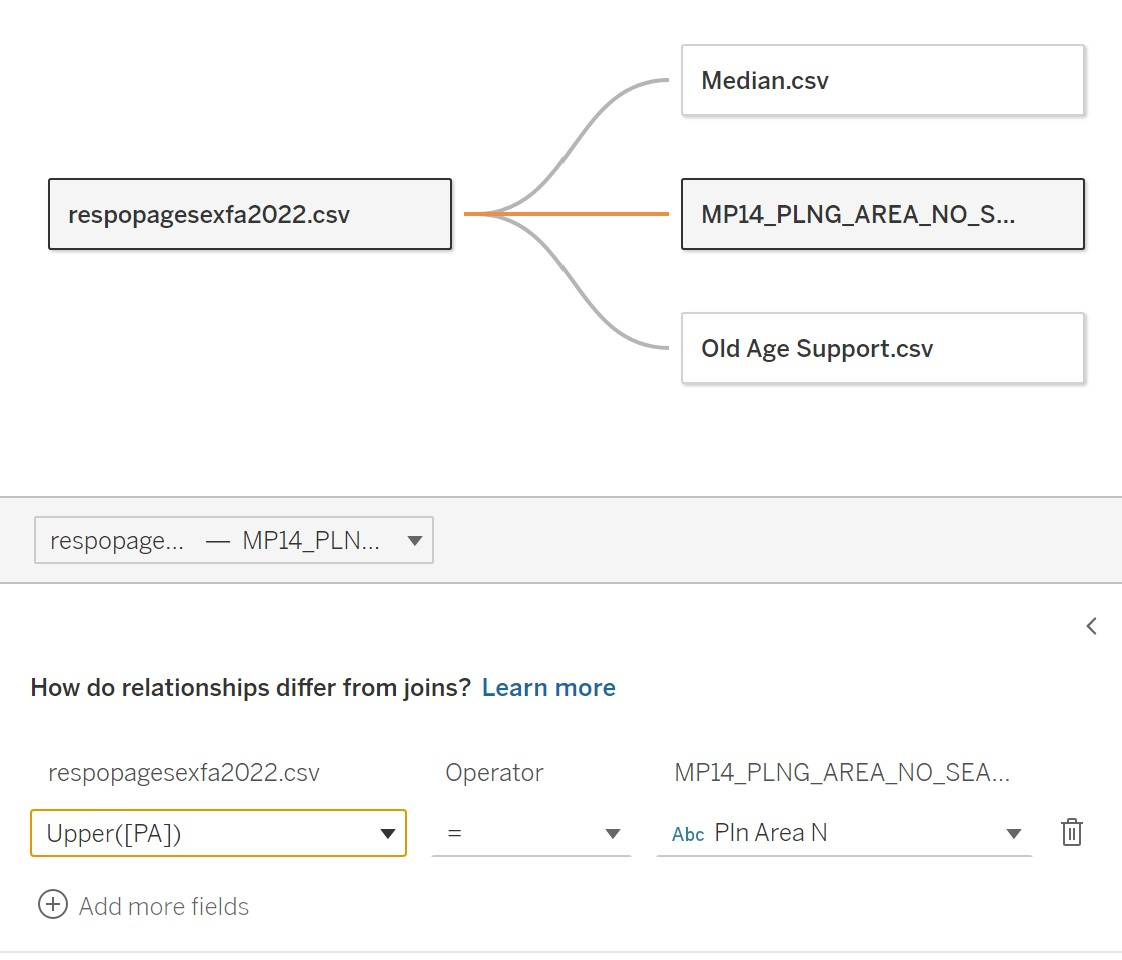
\includegraphics{images/join2.jpg} \\
4 & Drop Geometry to the field. & 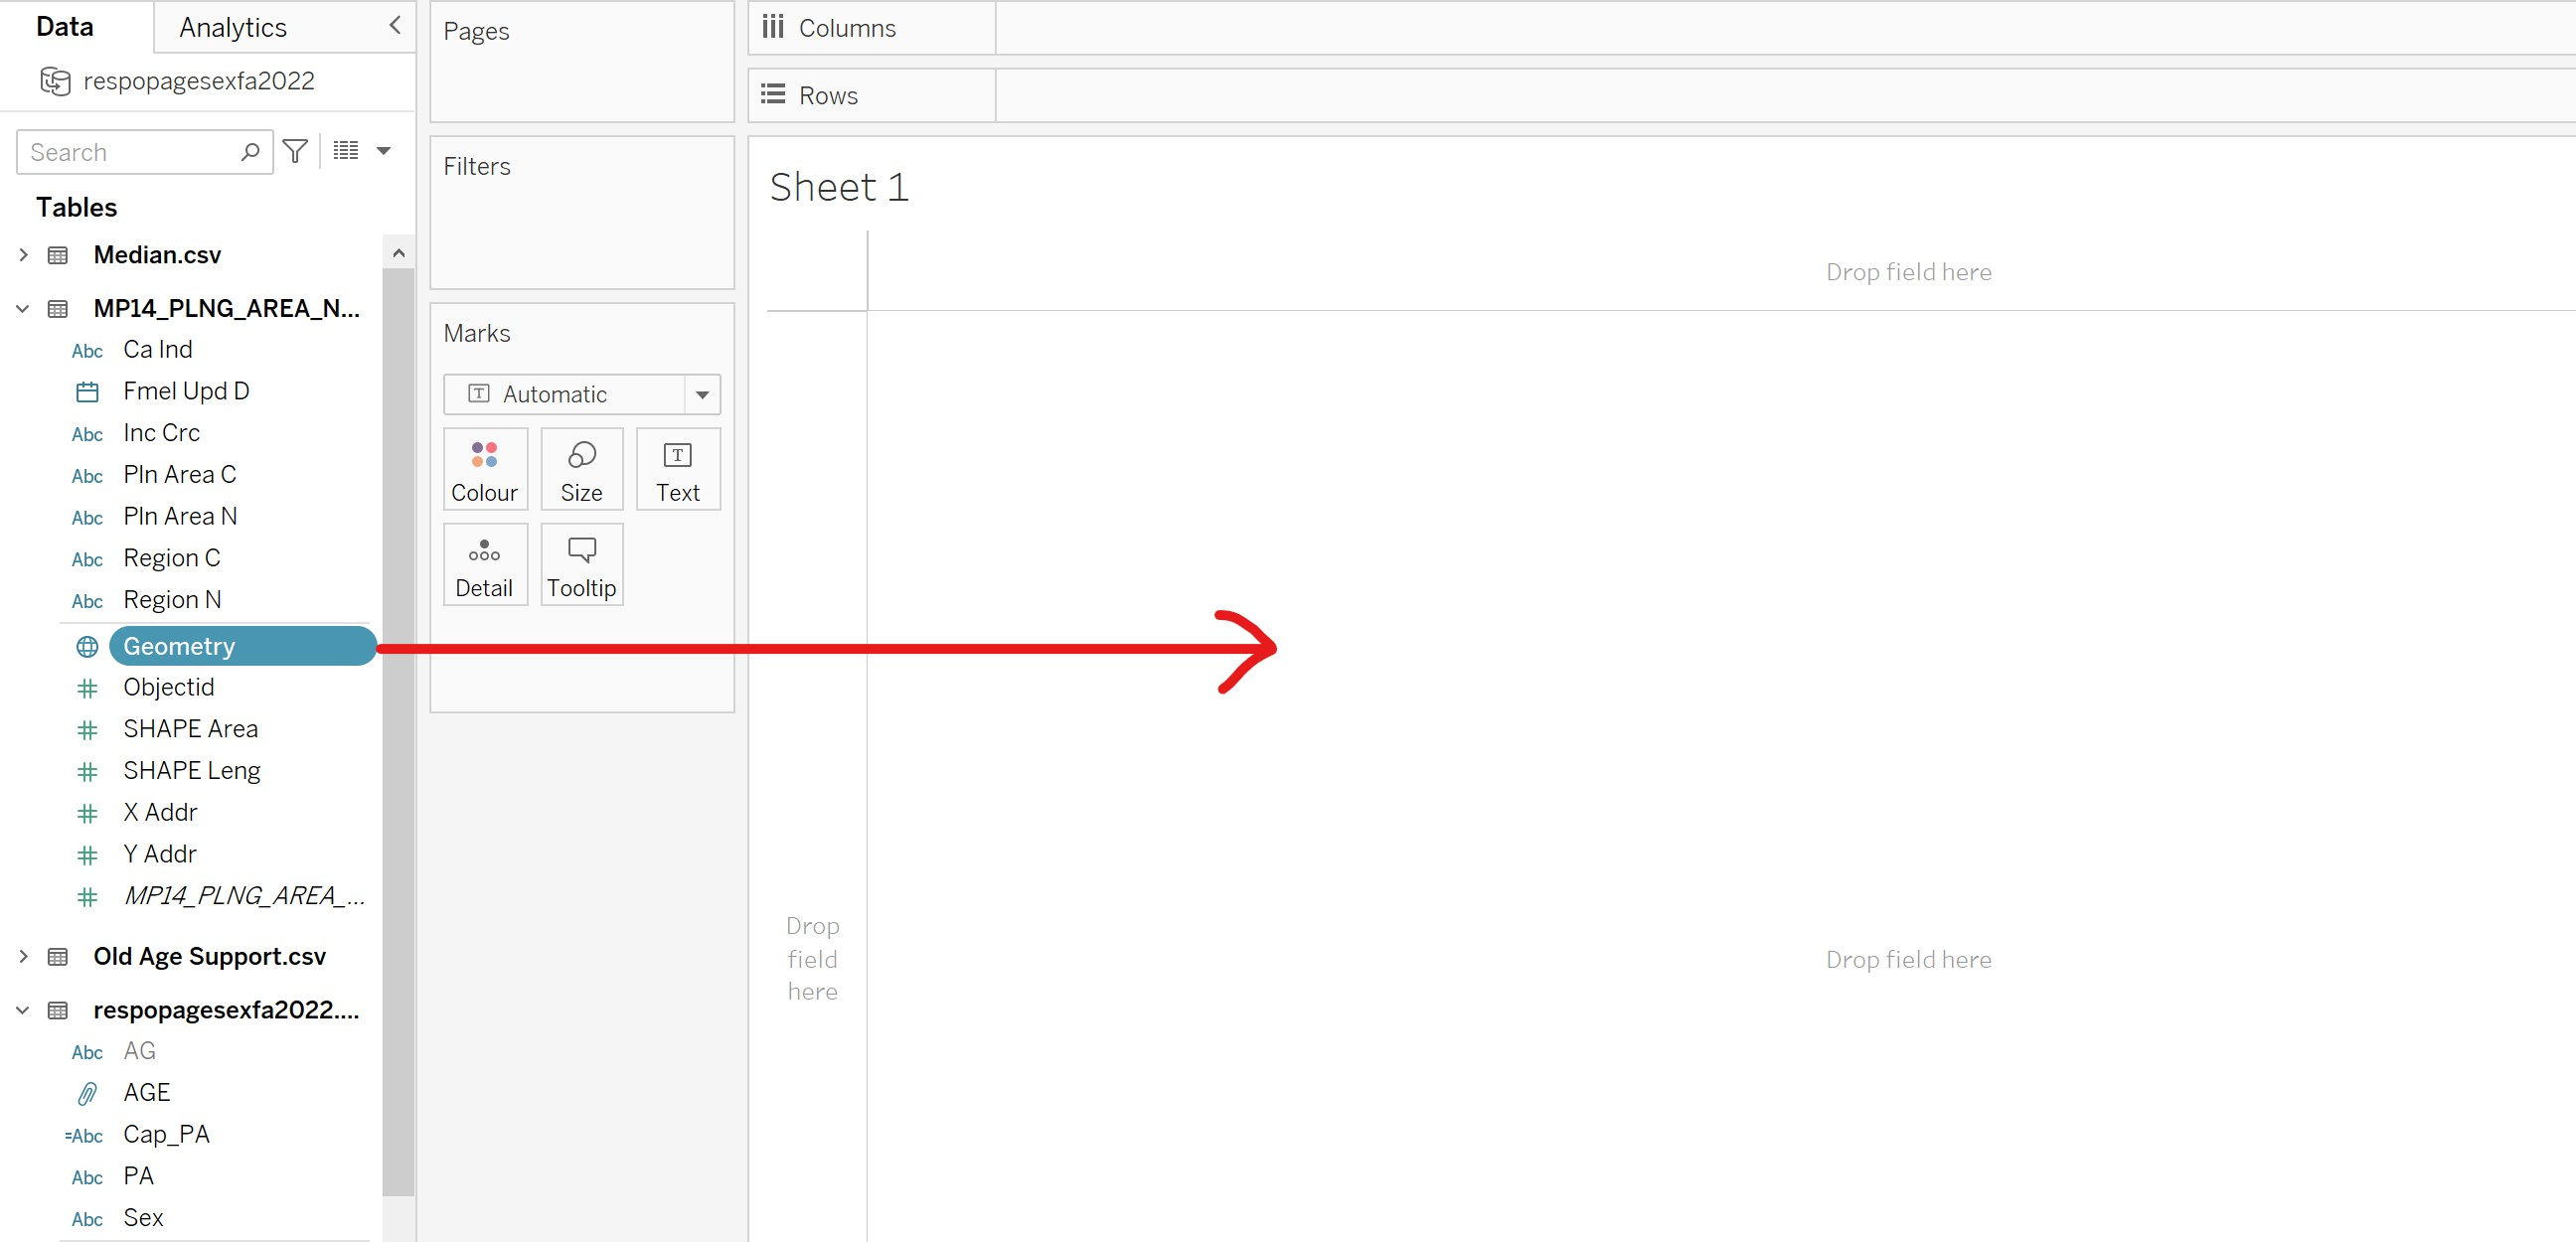
\includegraphics{images/drag.jpg} \\
5 & Drag Pop to Color, PA to Label. &
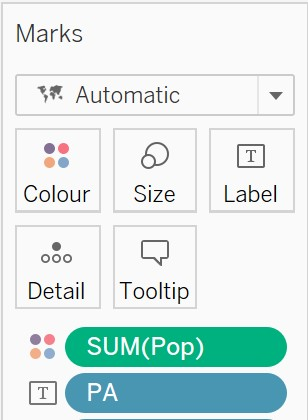
\includegraphics{images/drag to mark.jpg} \\
6 & Edit the color. When we choose step 3 and modify the color of least
population to light grey, the no. of highlighted region is 9. &
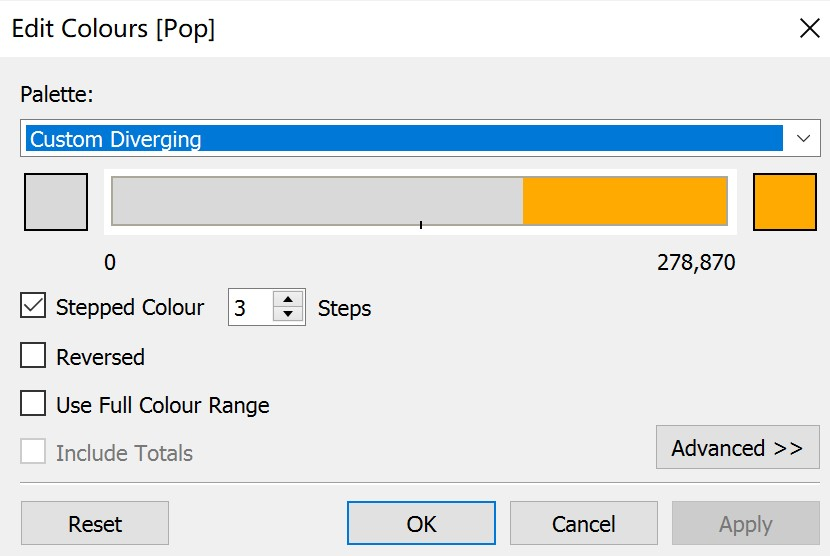
\includegraphics{images/color.jpg} \\
7 & Edit the label on the map. Select always show for Punggol and Bedok,
and never show for the rest PA. We can annotate the two highlighted
regions to facilitate understanding. &
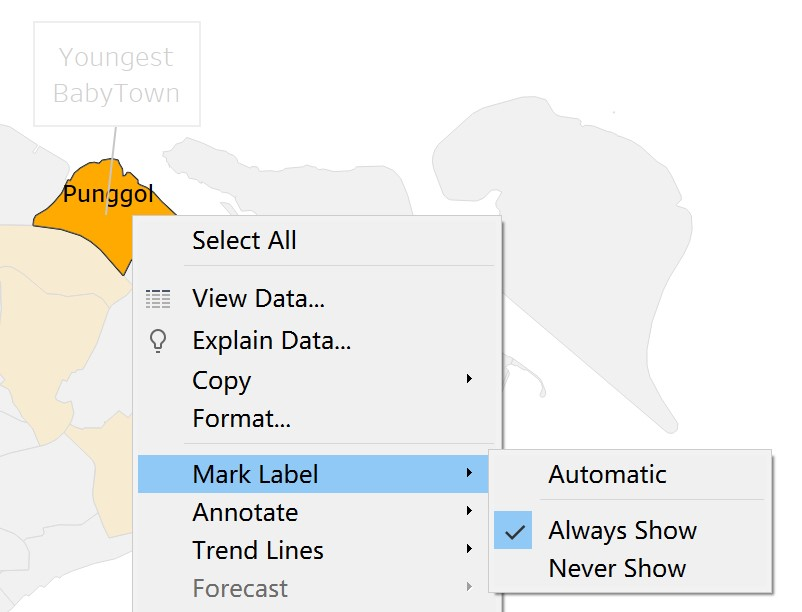
\includegraphics{images/always show.jpg} \\
\bottomrule()
\end{longtable}

\end{figure*}

\hypertarget{draw-pyramids-of-the-9-pas-and-display-in-trellis-single-diagram}{%
\subsubsection{4.2.2 Draw Pyramids of the 9 PAs and Display in Trellis
(single
diagram)}\label{draw-pyramids-of-the-9-pas-and-display-in-trellis-single-diagram}}

\begin{figure*}

\begin{longtable}[]{@{}
  >{\raggedright\arraybackslash}p{(\columnwidth - 4\tabcolsep) * \real{0.1000}}
  >{\raggedright\arraybackslash}p{(\columnwidth - 4\tabcolsep) * \real{0.3000}}
  >{\raggedright\arraybackslash}p{(\columnwidth - 4\tabcolsep) * \real{0.6000}}@{}}
\toprule()
\begin{minipage}[b]{\linewidth}\raggedright
No.
\end{minipage} & \begin{minipage}[b]{\linewidth}\raggedright
Step
\end{minipage} & \begin{minipage}[b]{\linewidth}\raggedright
Screenshot
\end{minipage} \\
\midrule()
\endhead
1 & Manually sort the PA (name of planning areas) based on median age as
we would like to control the arrangement of pyramids of PA in trellis. &
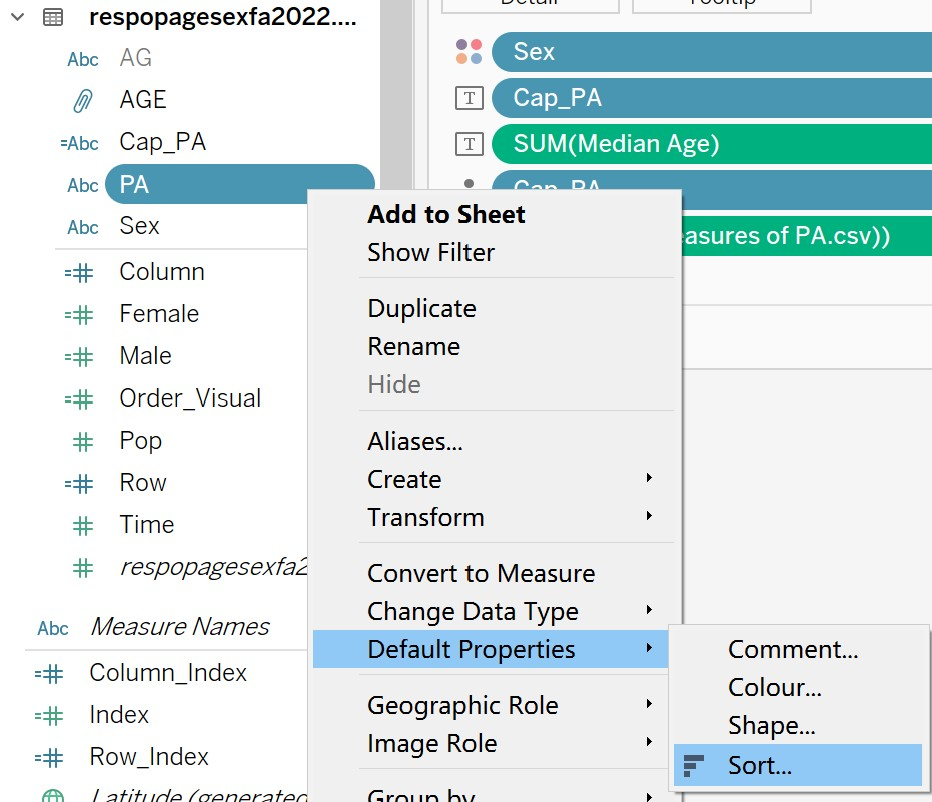
\includegraphics{images/sort pa-01.jpg} \\
2 & The 9 most populated PA are sorted, while the rest of PA are
unchanged. & 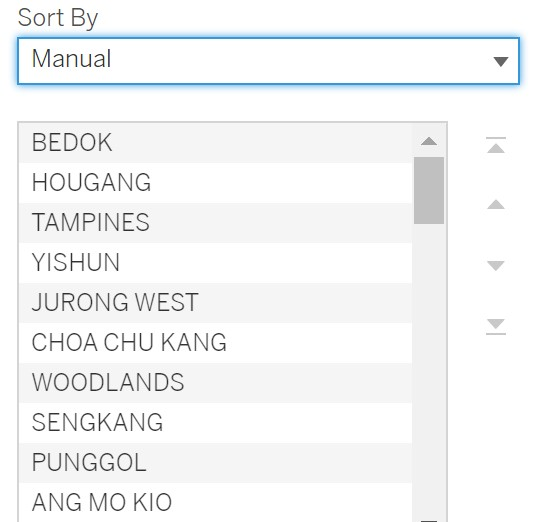
\includegraphics{images/sorted pa-01.jpg} \\
3 & Create a new parameter representing the number of columns in
trellis. In this example, the parameter should be sqrt(9) = 3. Note that
creating such parameter is to avoid hard code. &
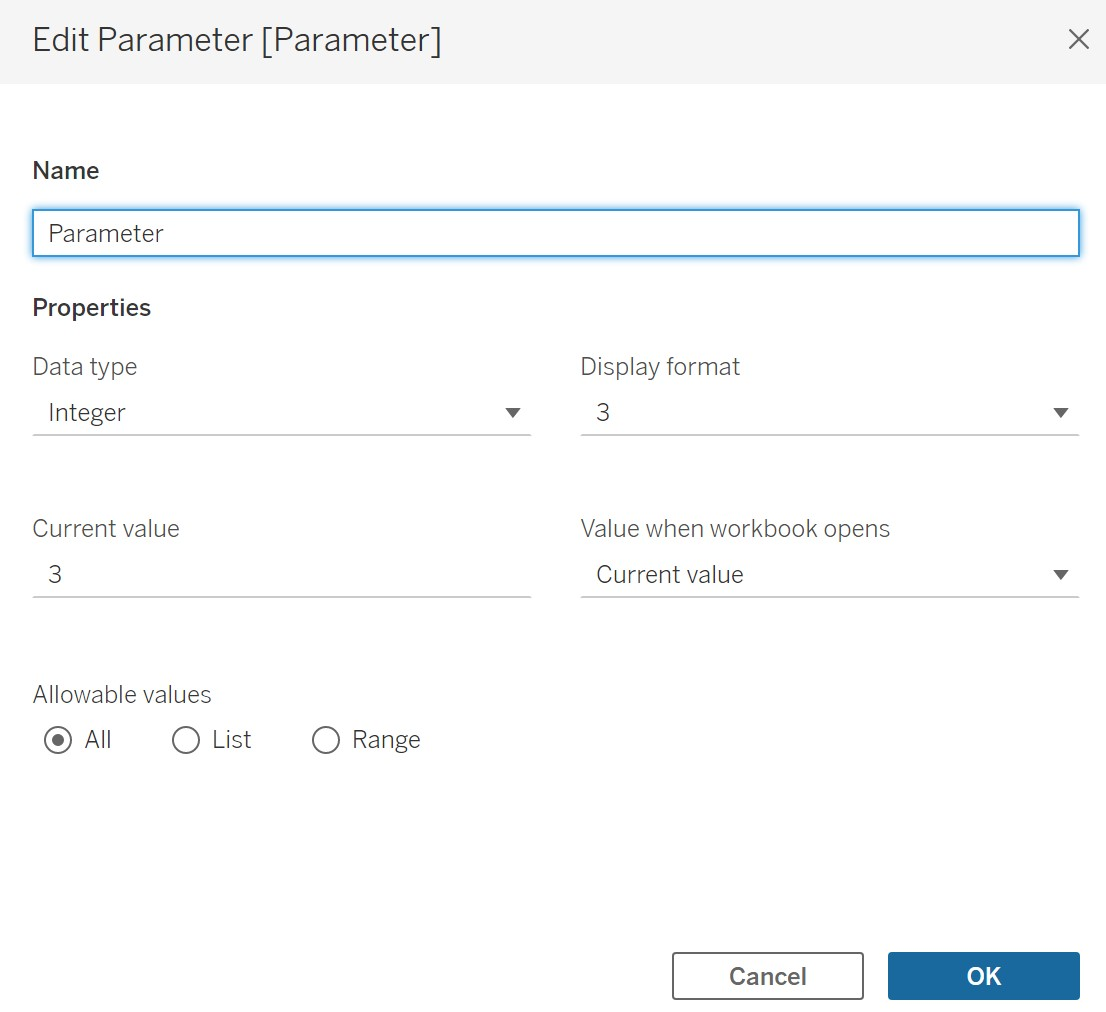
\includegraphics{images/parameter.jpg} \\
4 & Create a new calculated field named Index of each row. &
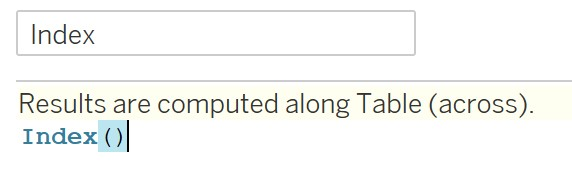
\includegraphics{images/index.jpg} \\
5 & Create a new calculated field named Column Index of each row. &
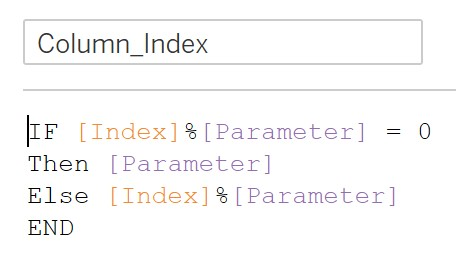
\includegraphics{images/column index.jpg} \\
6 & Create a new calculated field named Row Index of each row. Note that
the column index and row index will be used when we need to display the
9 pyramids in trellis (a single diagram containning many small plots).
The two index serve the purpose as the coordinate of each small plot,
such as (1,1) in the top left corner and (3,3) in the bottom right
corner. & 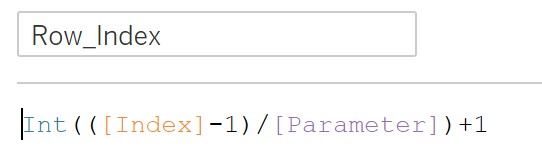
\includegraphics{images/row_index.jpg} \\
7 & As we would like to display partial data in trellis, we created a
new calculated field called Group1 to group the 9 selected PA in one
group, & 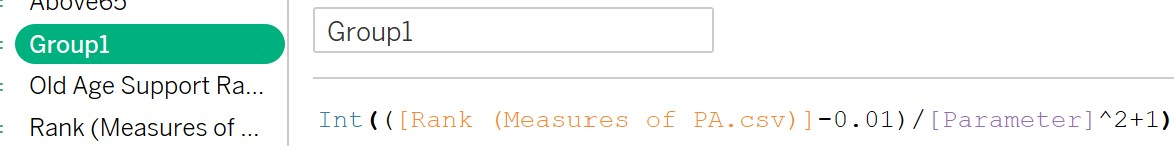
\includegraphics{images/Group1.jpg} \\
8 & Then we drop Group1, choose Attribute to filter and select `1' only.
& 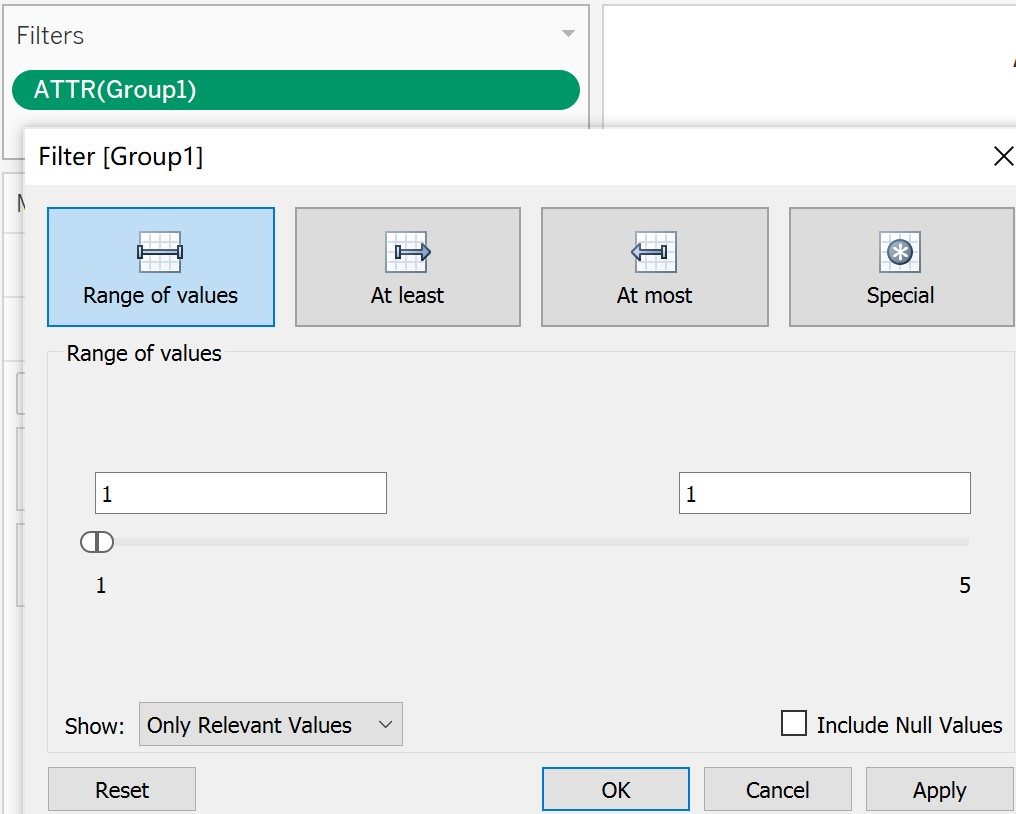
\includegraphics{images/filter group1.jpg} \\
9 & Due to space constrain, we create new age groups. In the original
dataset, the step between consecutive age groups is 5. We increase it to
10. That is, we combine every 2 groups into 1, such as 0 to 4 and 5 to 9
into 0 to 9. & 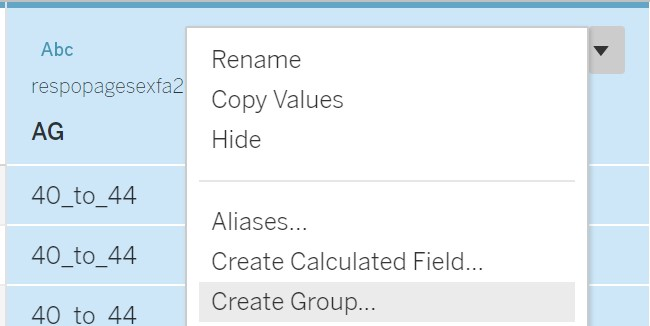
\includegraphics{images/create new age group.jpg}

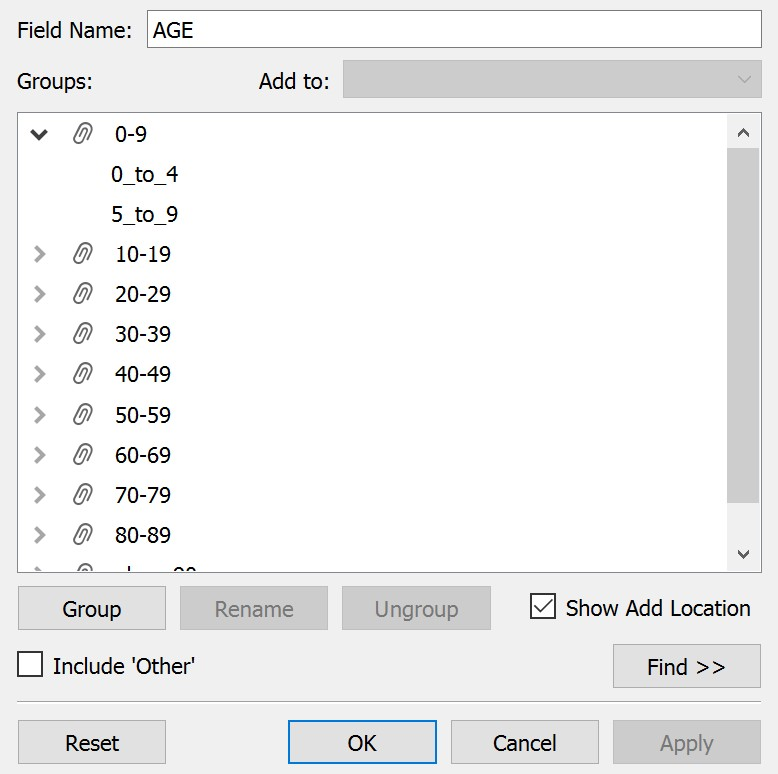
\includegraphics{images/new age group.jpg} \\
10 & Create new calculated field of population of males and females as
shown. & 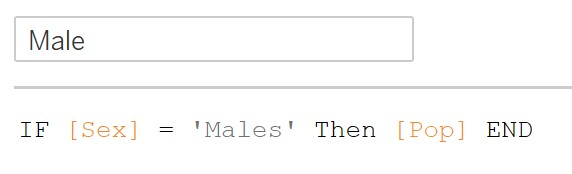
\includegraphics{images/Male.jpg}

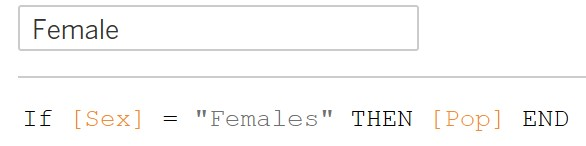
\includegraphics{images/Female.jpg} \\
11 & Drop Row\_Index, Male and Female into Columns.

Drop Column\_Index and AGE into Rows.

Drop PA to Detail.

Note that we need to modify the Row\_Index and Column\_Index by
selecting computing using PA. &
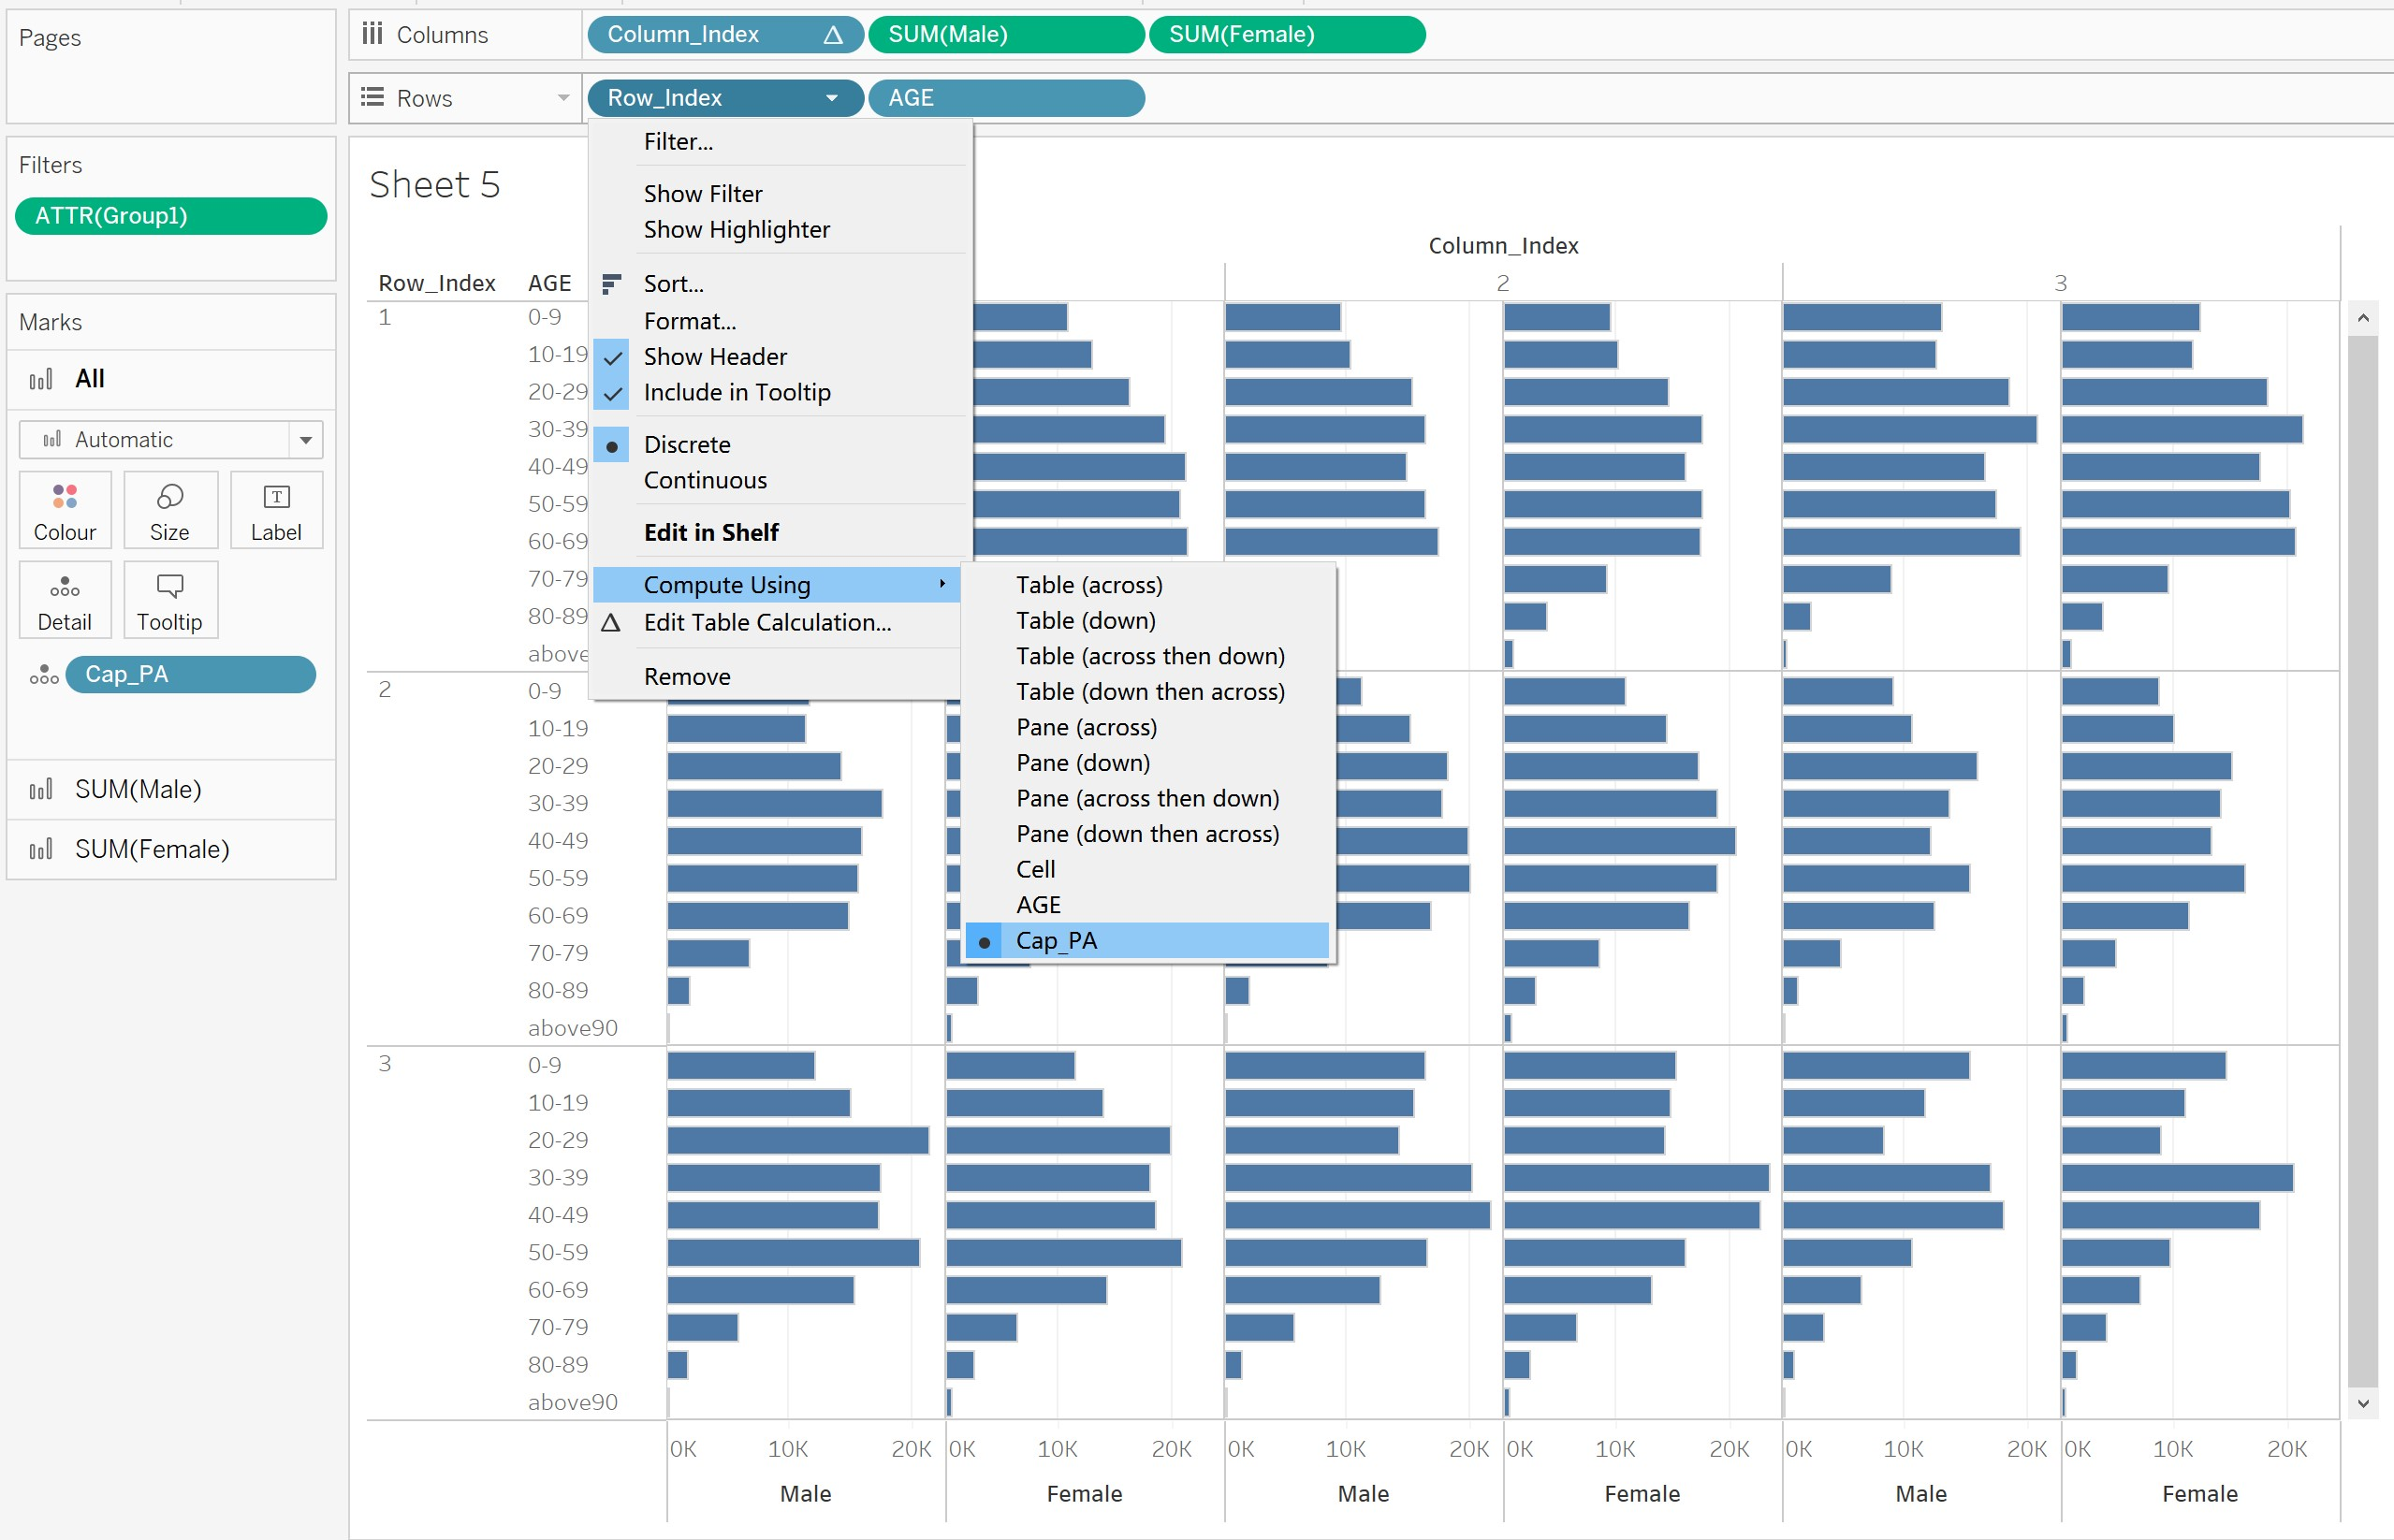
\includegraphics{images/Base of the main dashboard.jpg} \\
12 & Then we drop the {[}Sex{]} to Colour, Rank of PA to Detail in Mark
card of All. We can modify the color of sex by using blue to represent
Male and Pink to represent Female. &
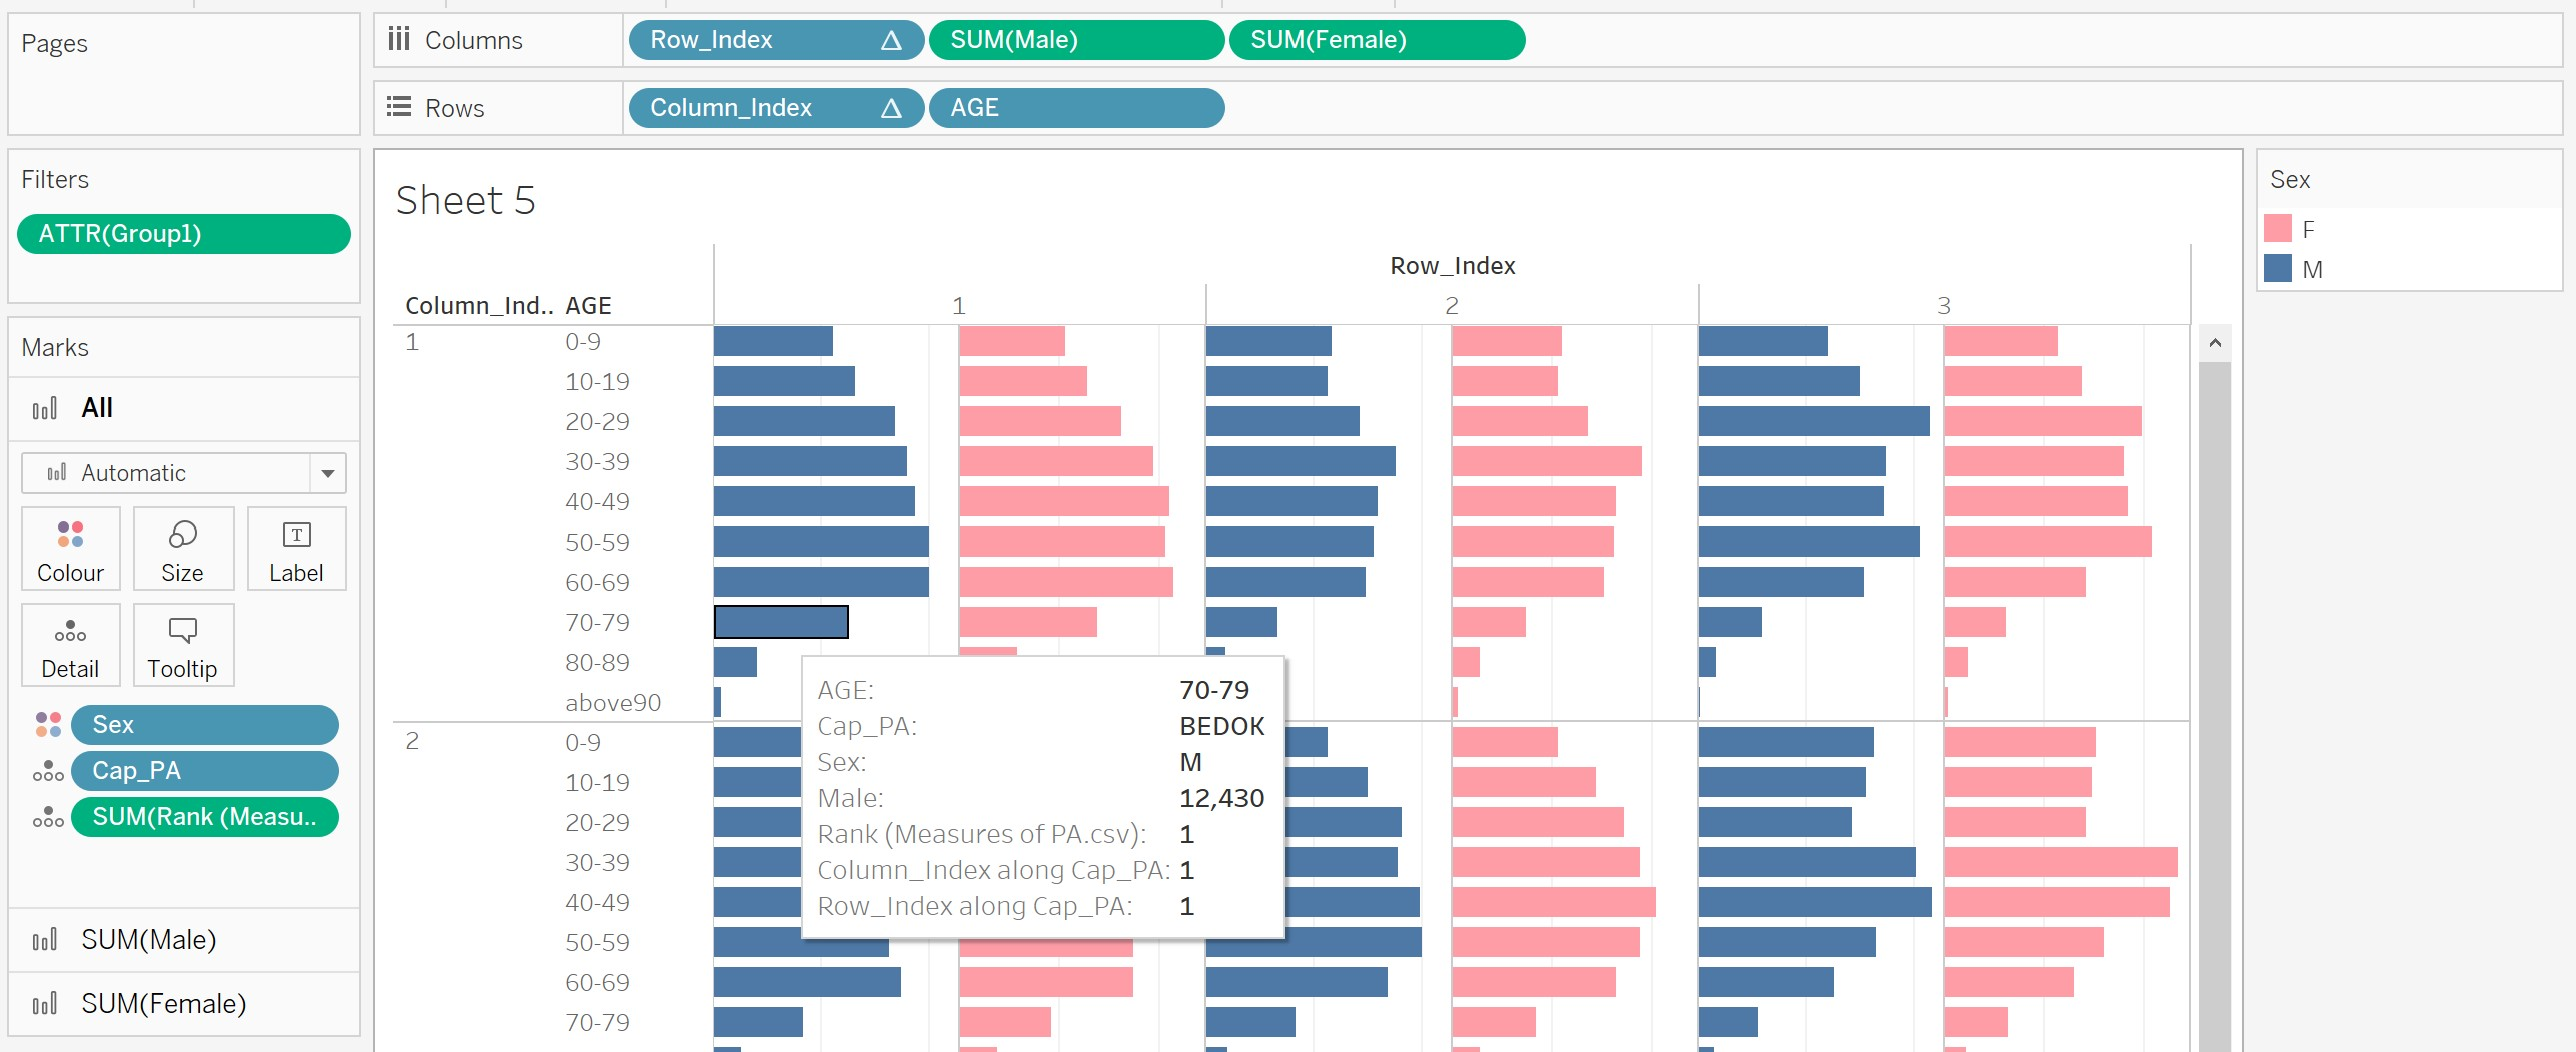
\includegraphics{images/change color.jpg} \\
13 & Modify the tooltip. & 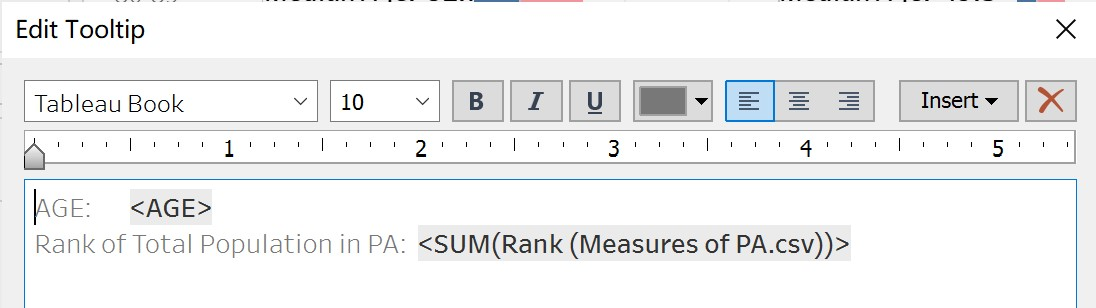
\includegraphics{images/tooltip.jpg} \\
14 & Rearrange the order of age group on y axis. &
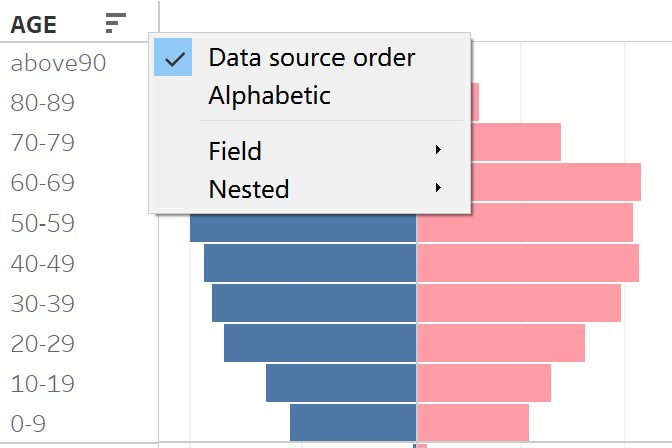
\includegraphics{images/rearrange the order of age.jpg} \\
15 & Add the label for the bar representing age group of 90+ for Males
in each PA.

First, select all bars and choose Mark Label -\textgreater{} Never Show.

Then select the bars representing age group of 90+ and choose Mark Label
-\textgreater{} Always Show. & 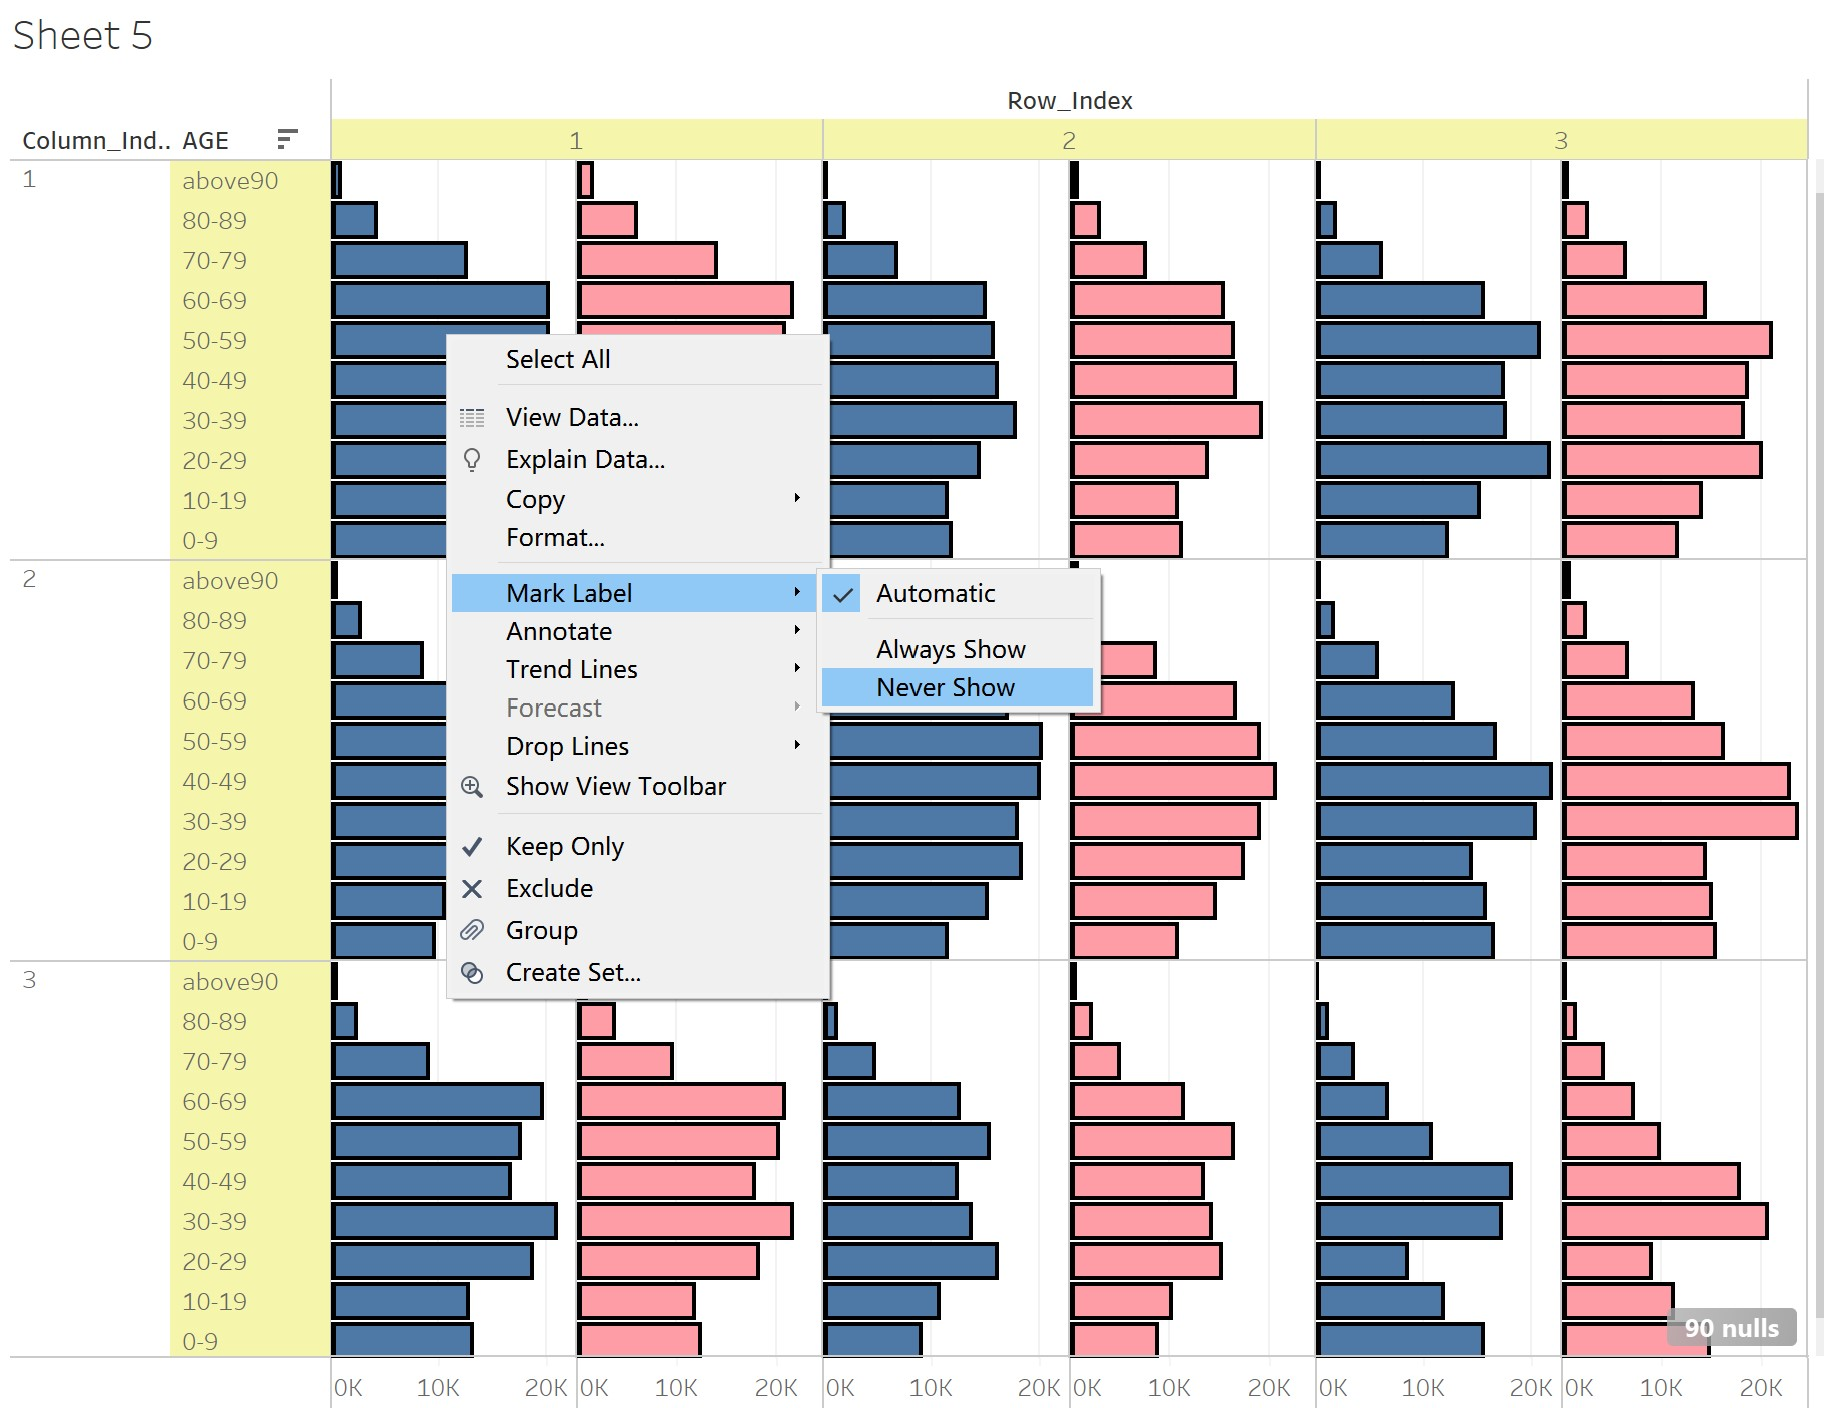
\includegraphics{images/add label 0.jpg}

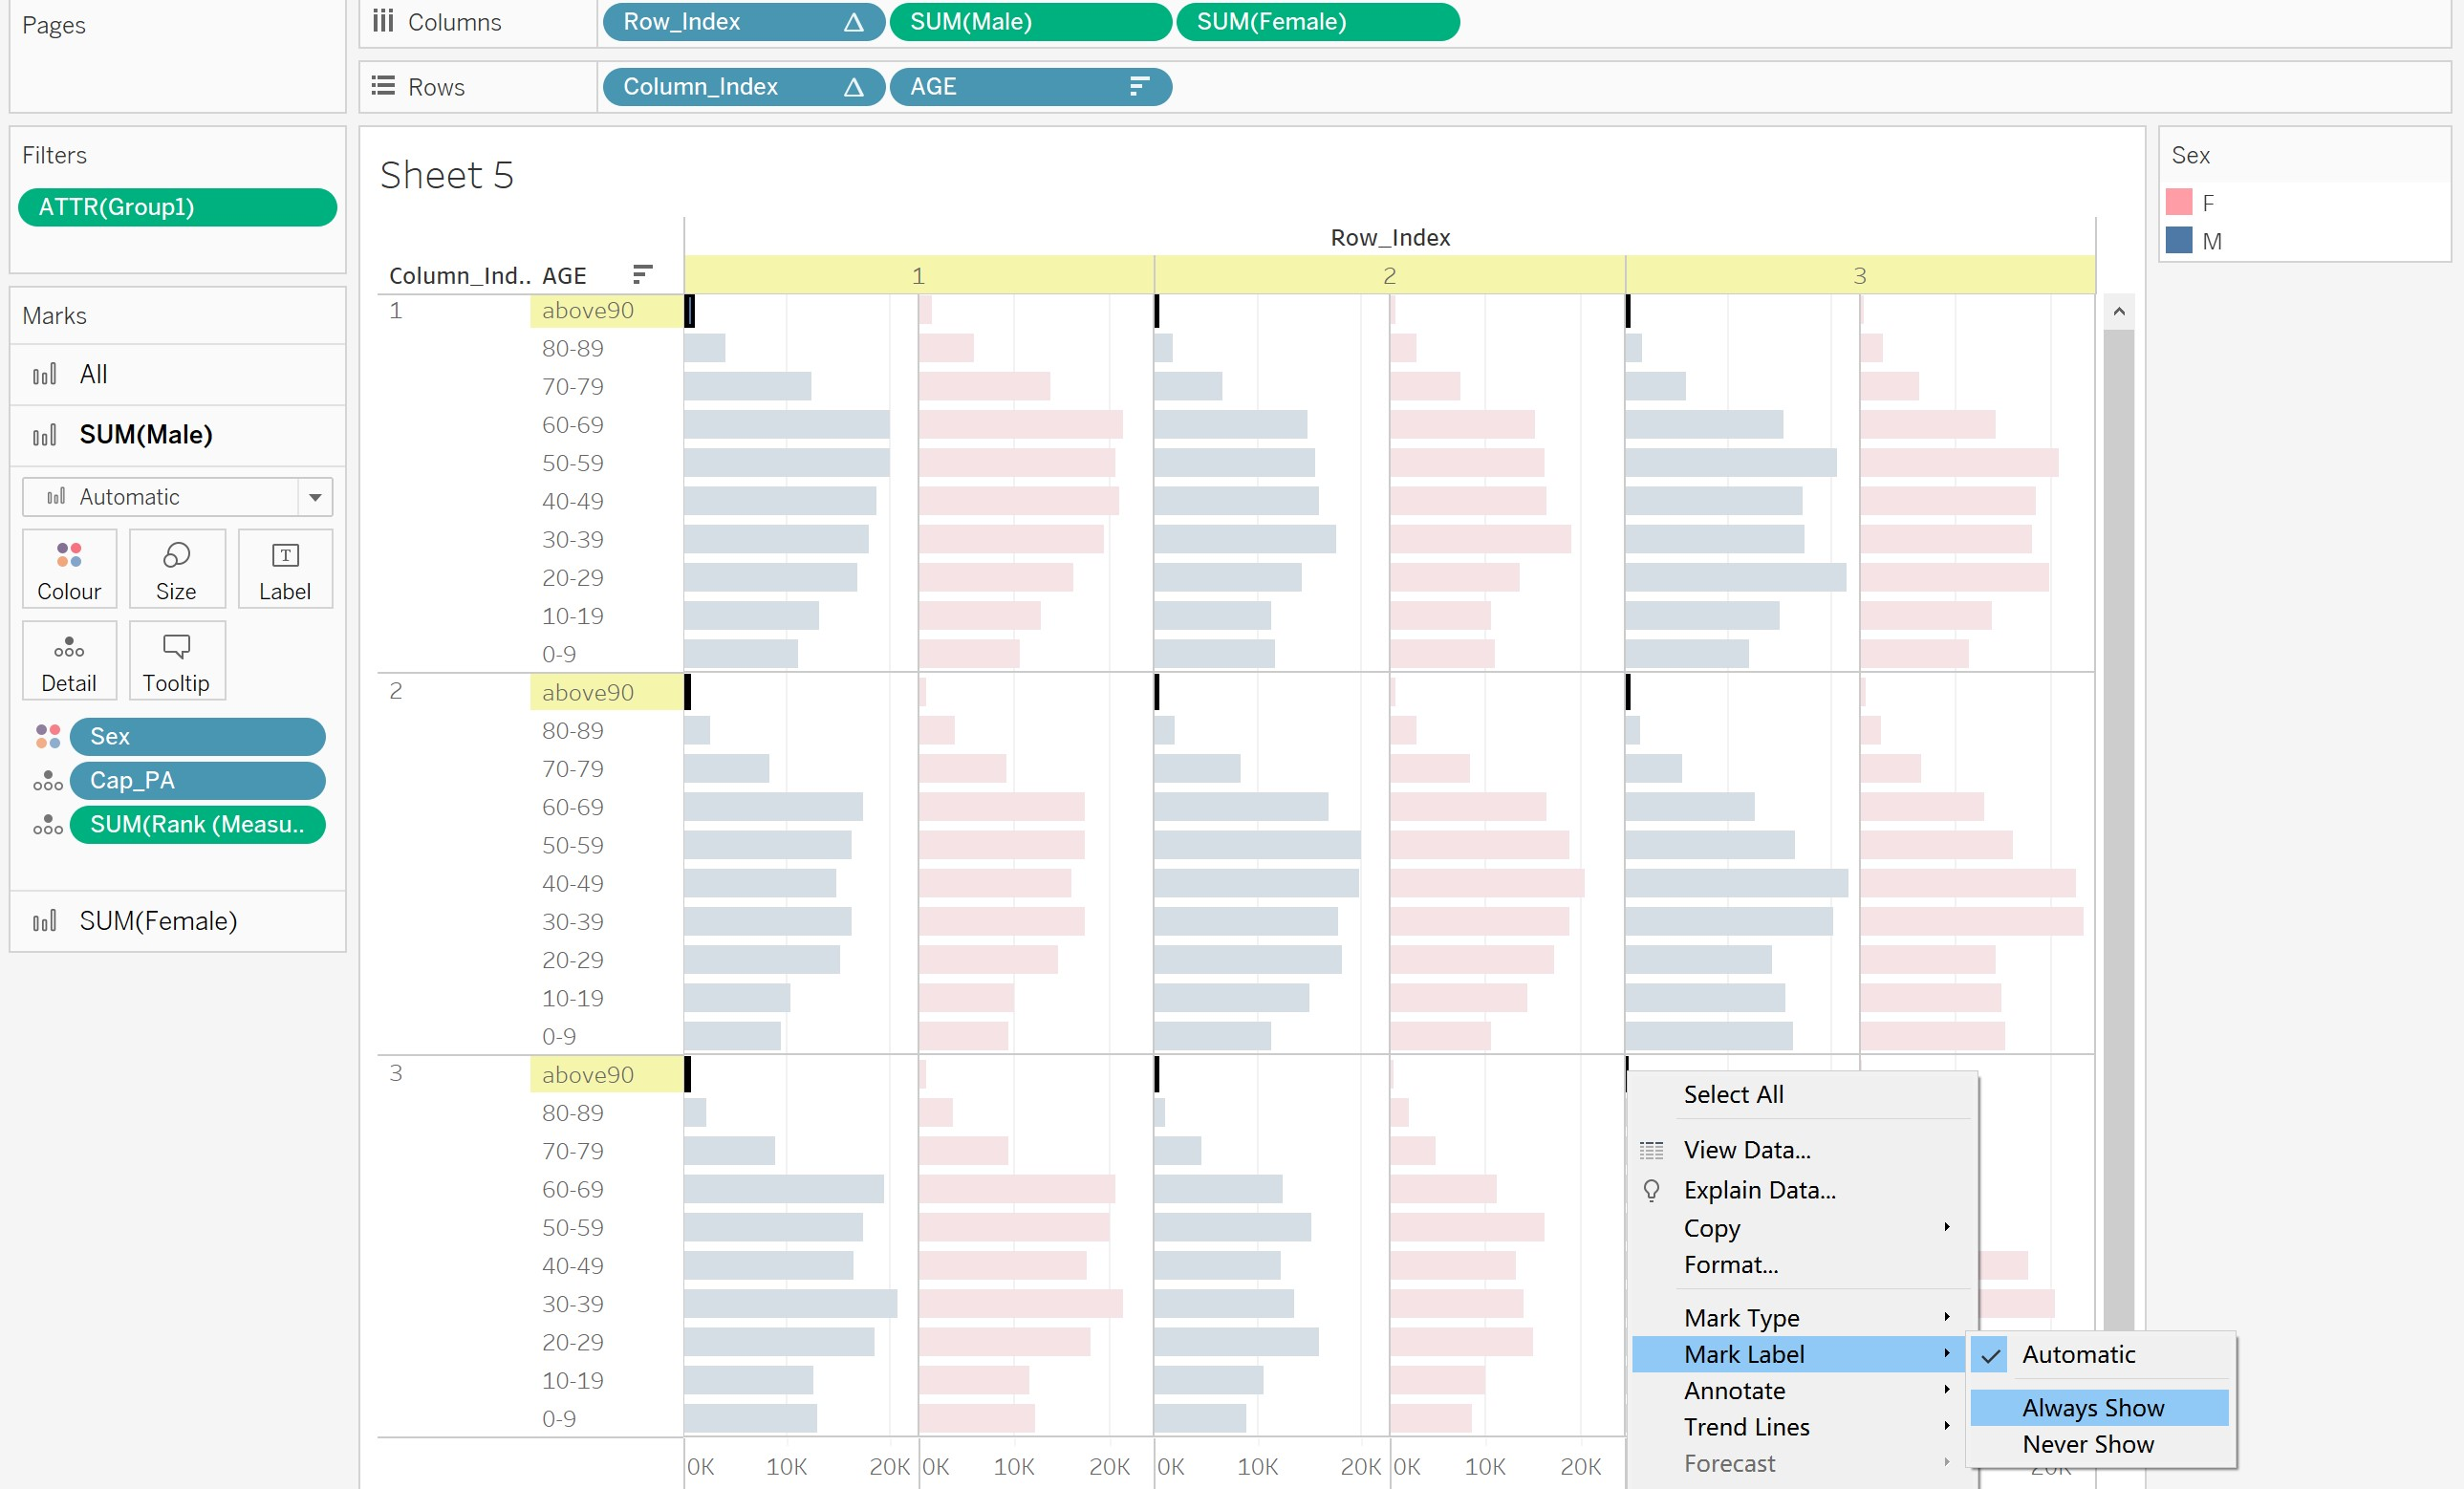
\includegraphics{images/add label 1.jpg} \\
16 & Then add names of PA and median age of PA to Labels. &
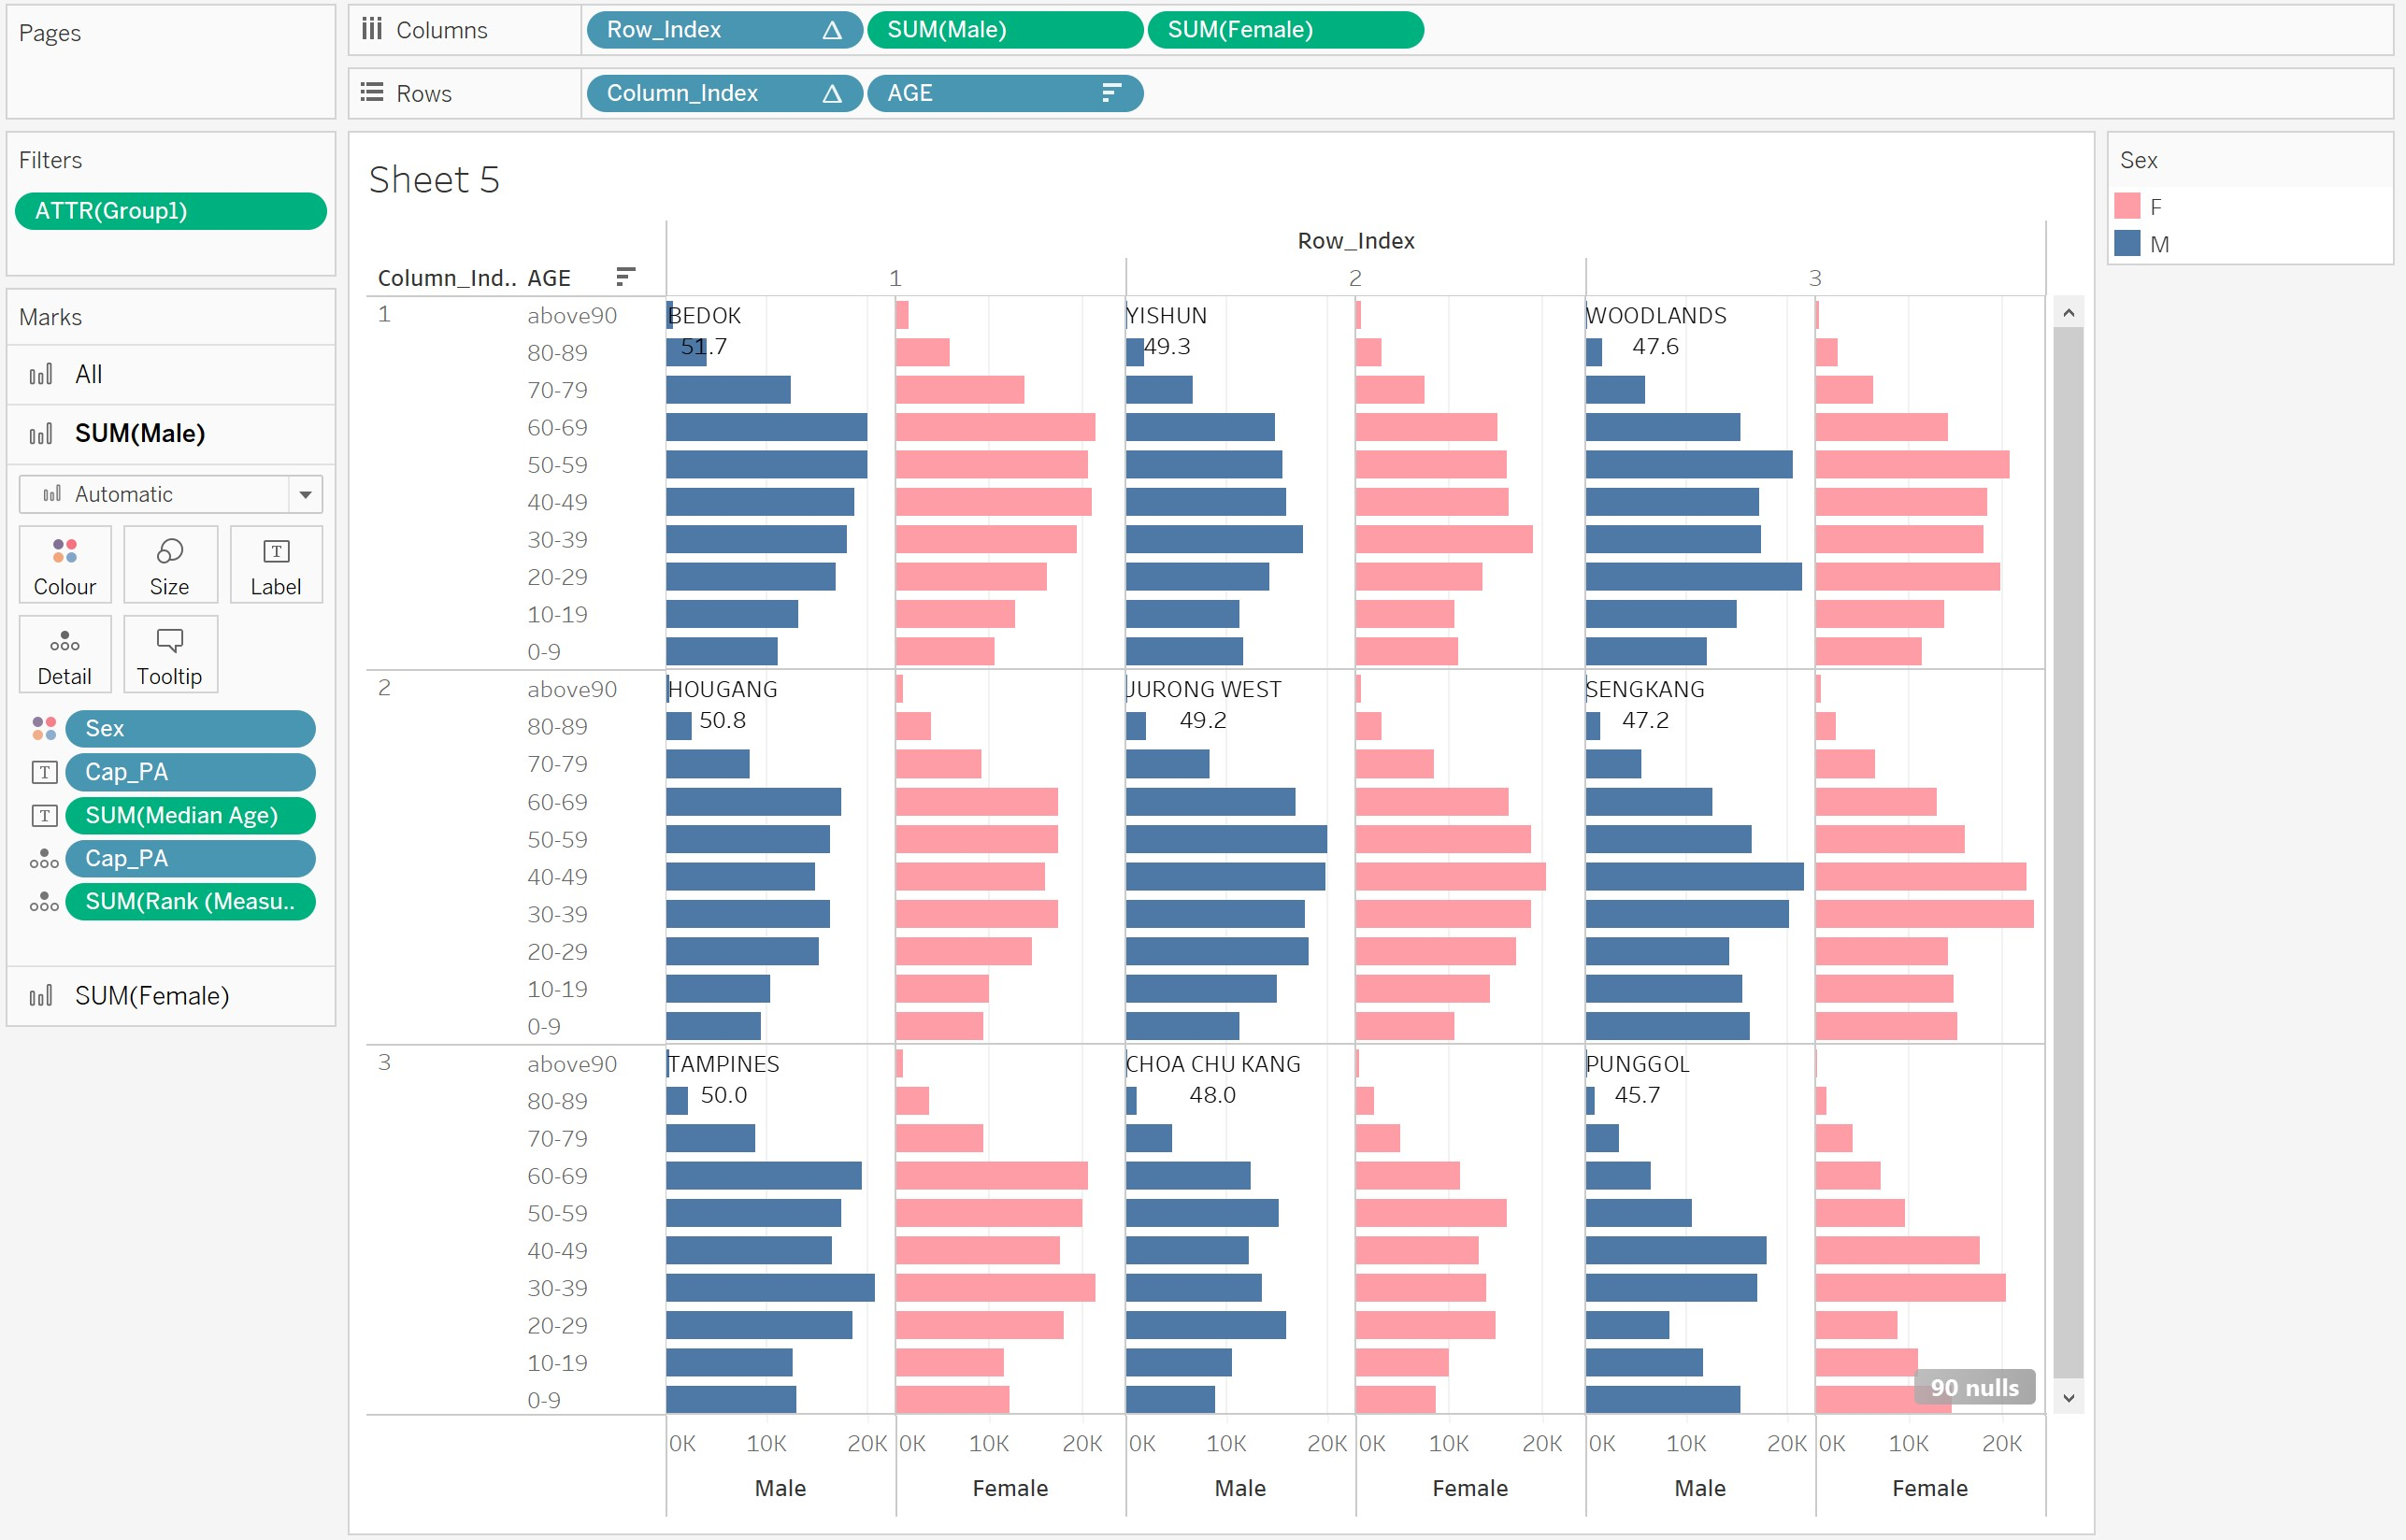
\includegraphics{images/just need to reverse.jpg} \\
17 & Reverse the Male axis to build pyramid. &
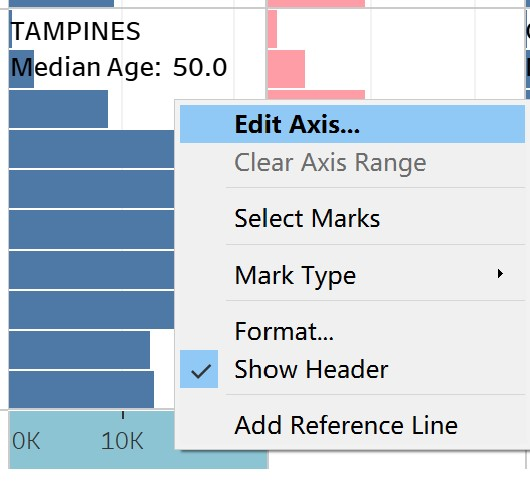
\includegraphics{images/reverse the male x-axis.jpg}

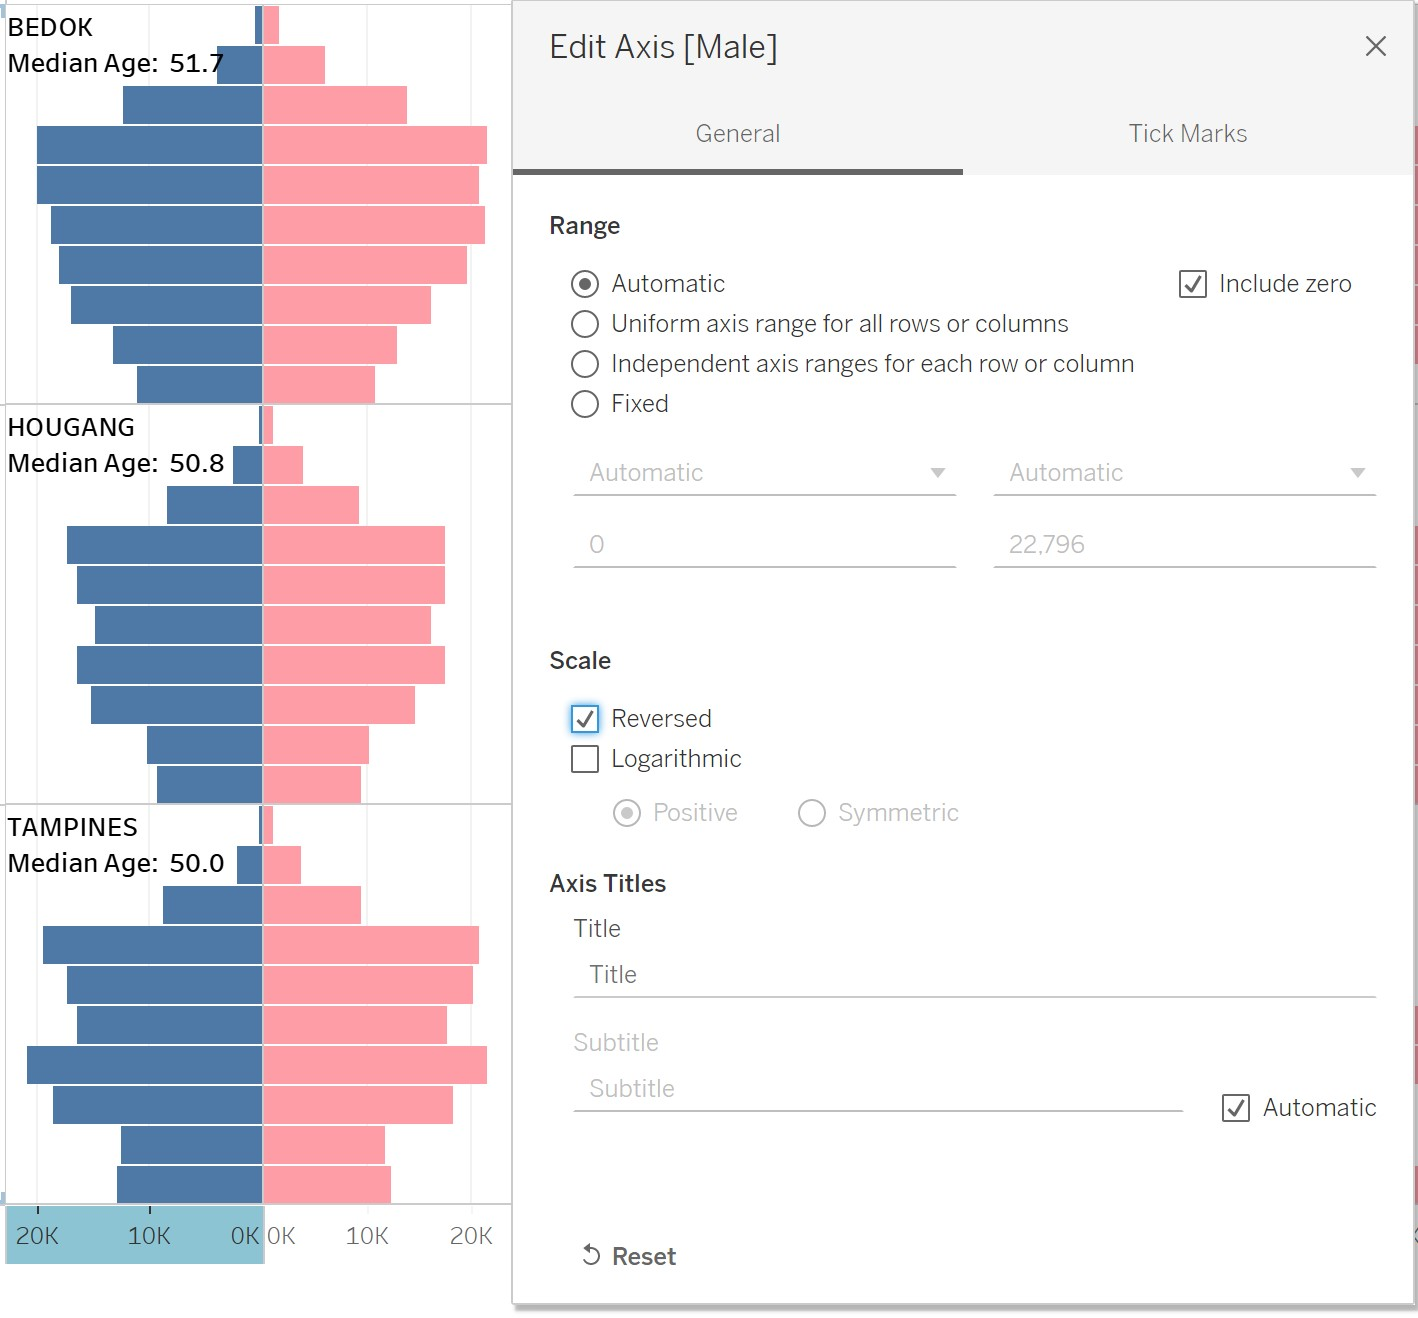
\includegraphics{images/reversed.jpg} \\
18 & Format of label by click the `\ldots{}' as shown on the screenshot.

Please note that in order for the label to appear on the top left
corner, I specifically add a full stop of blue color after many empty
spaces in the second line. & 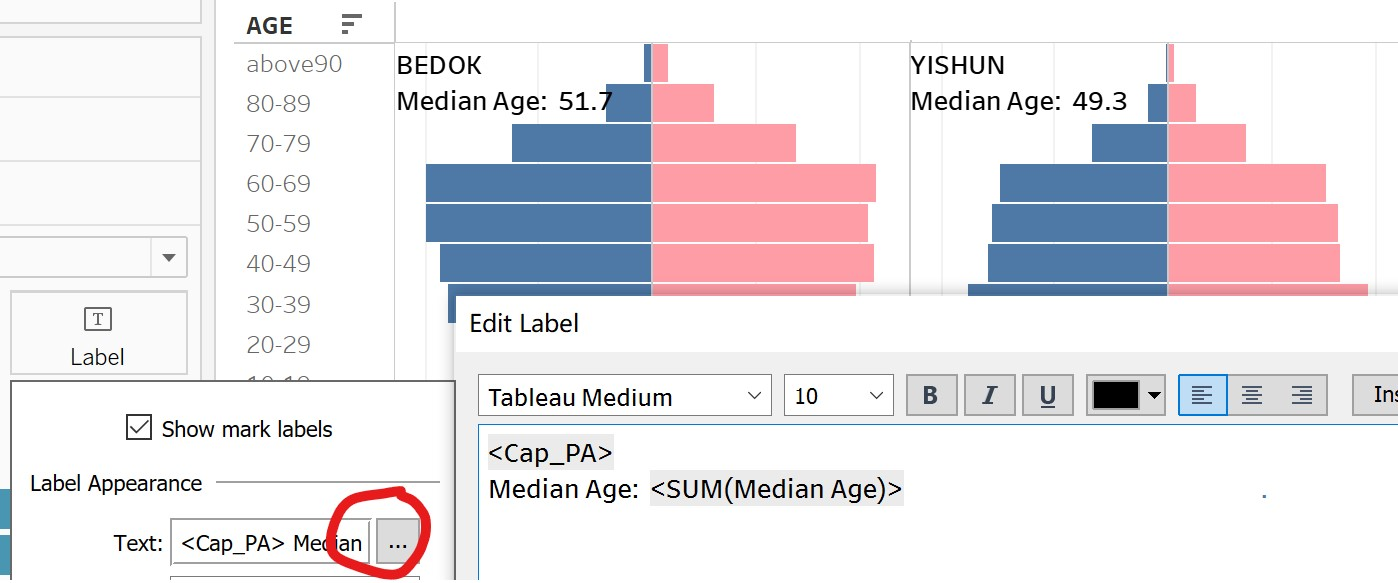
\includegraphics{images/formating 1.jpg} \\
19 & Add the title of the worksheet.

Remove the unnecessary headers to obtain the final view of the
worksheet. & 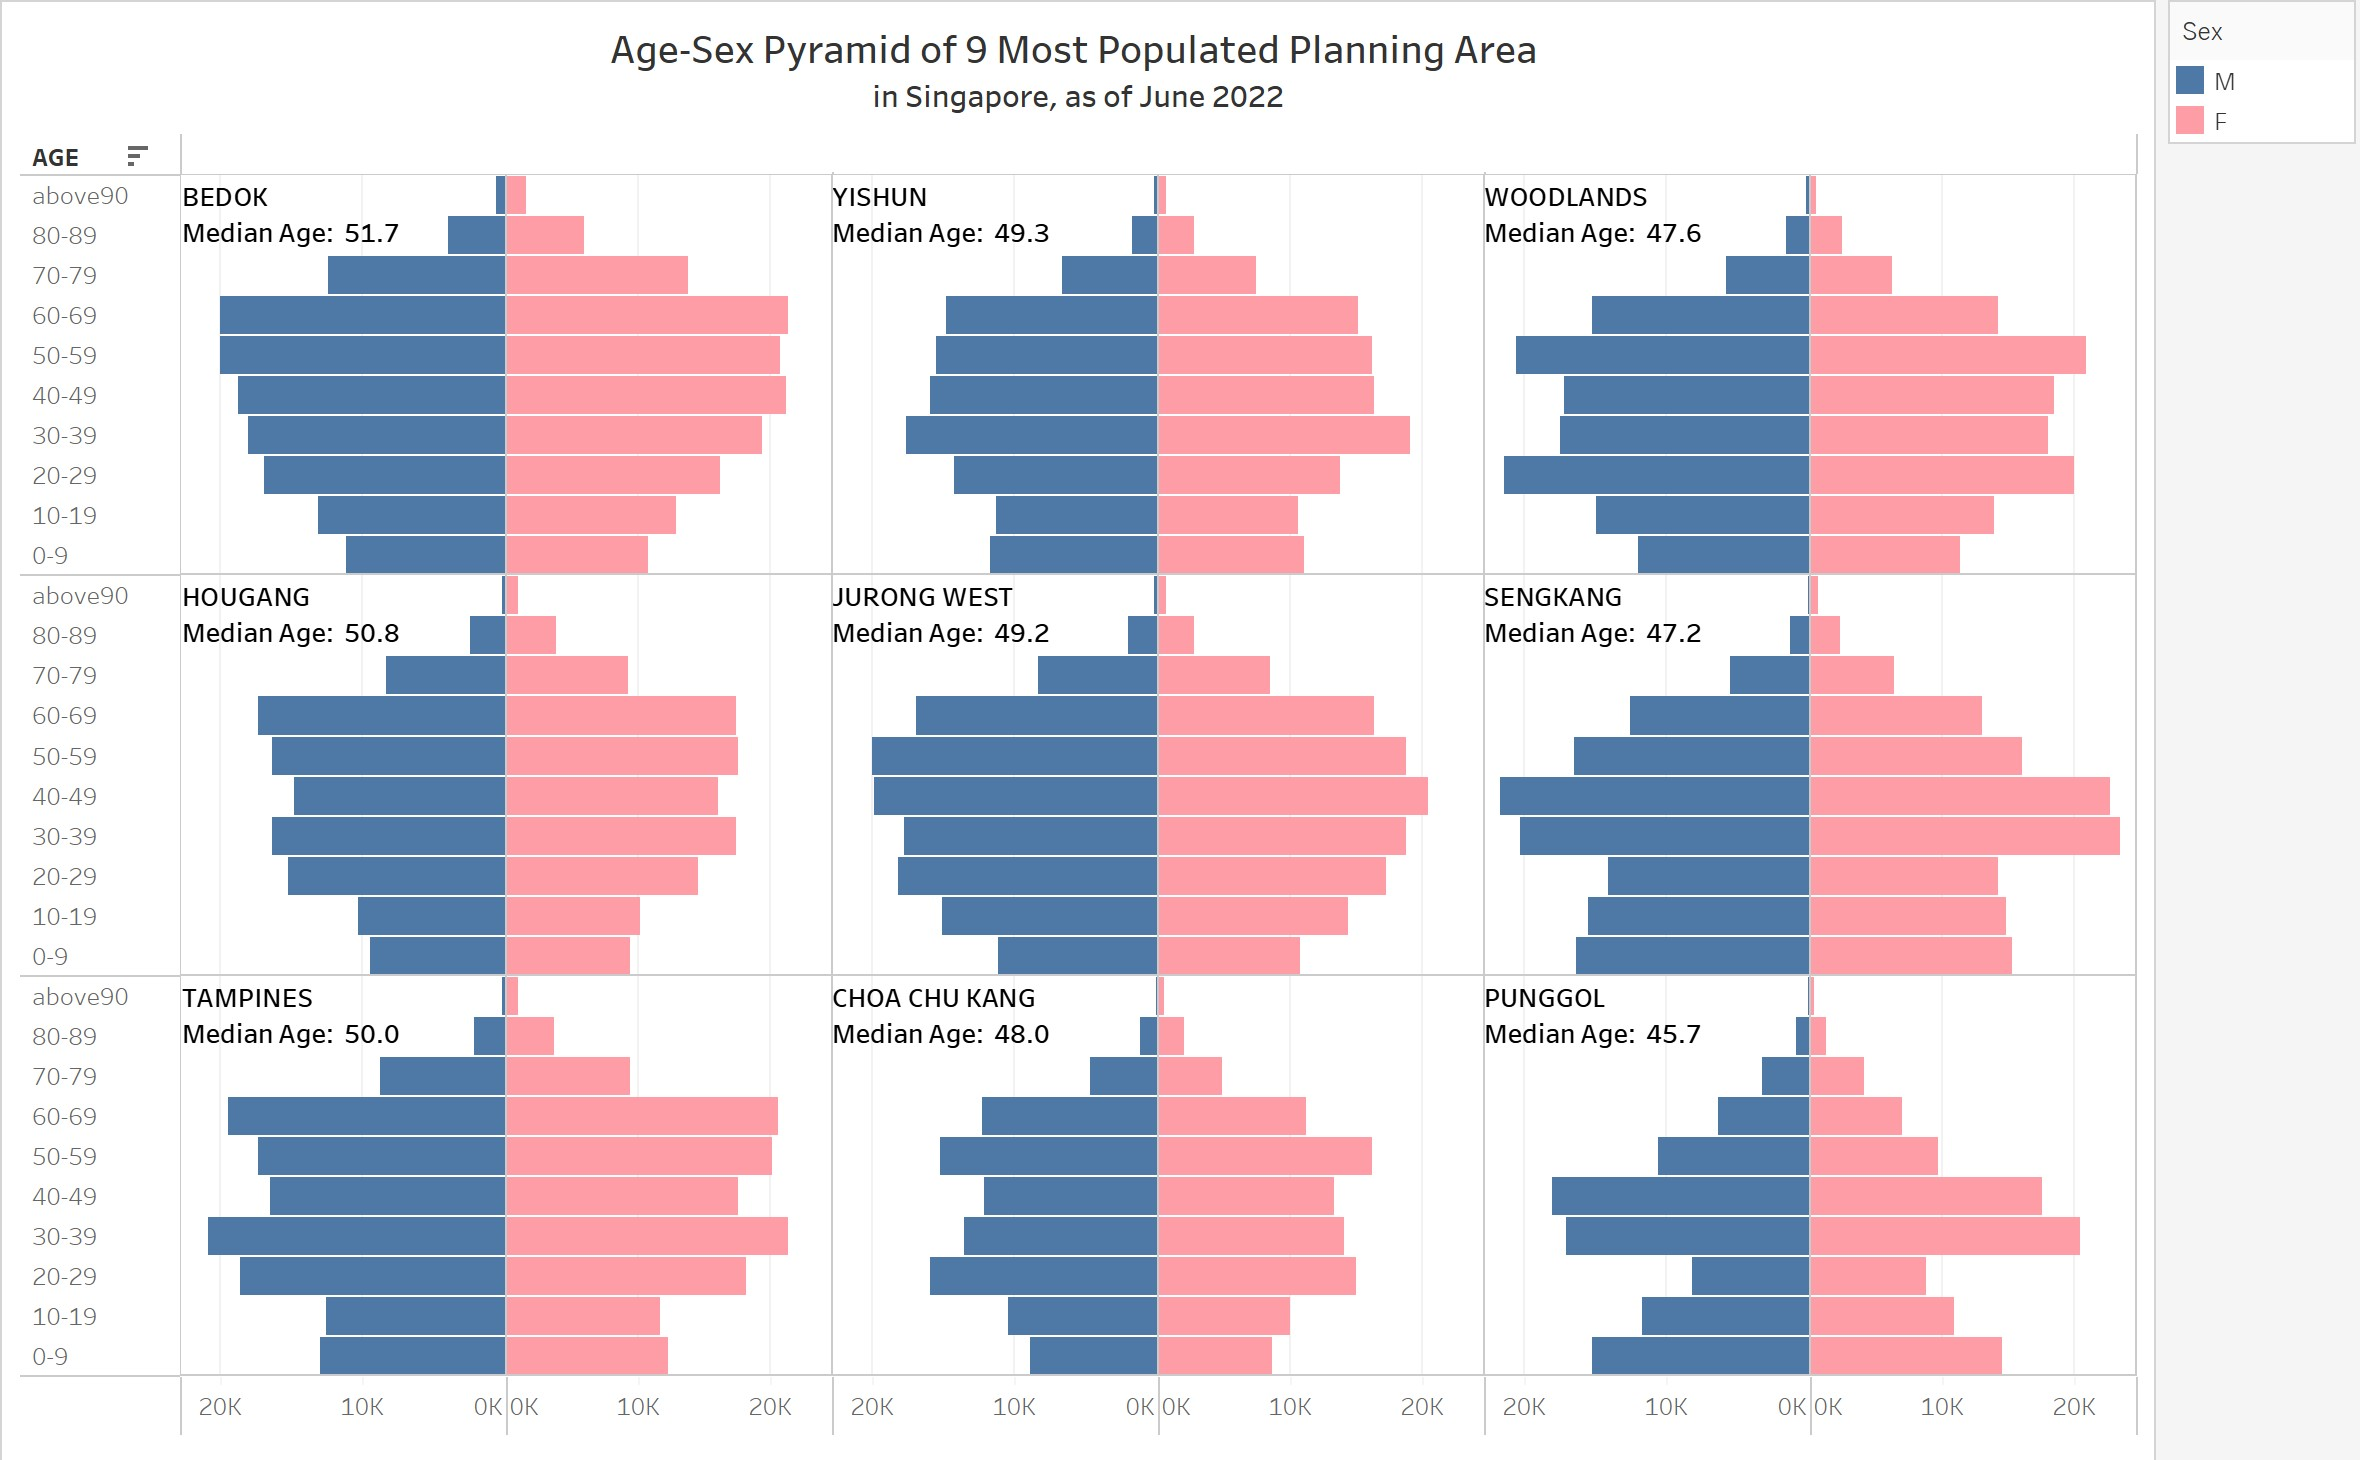
\includegraphics{images/final main.jpg} \\
20 & Create a new worksheet to plot the pyramid of Singapore as a
reference. & 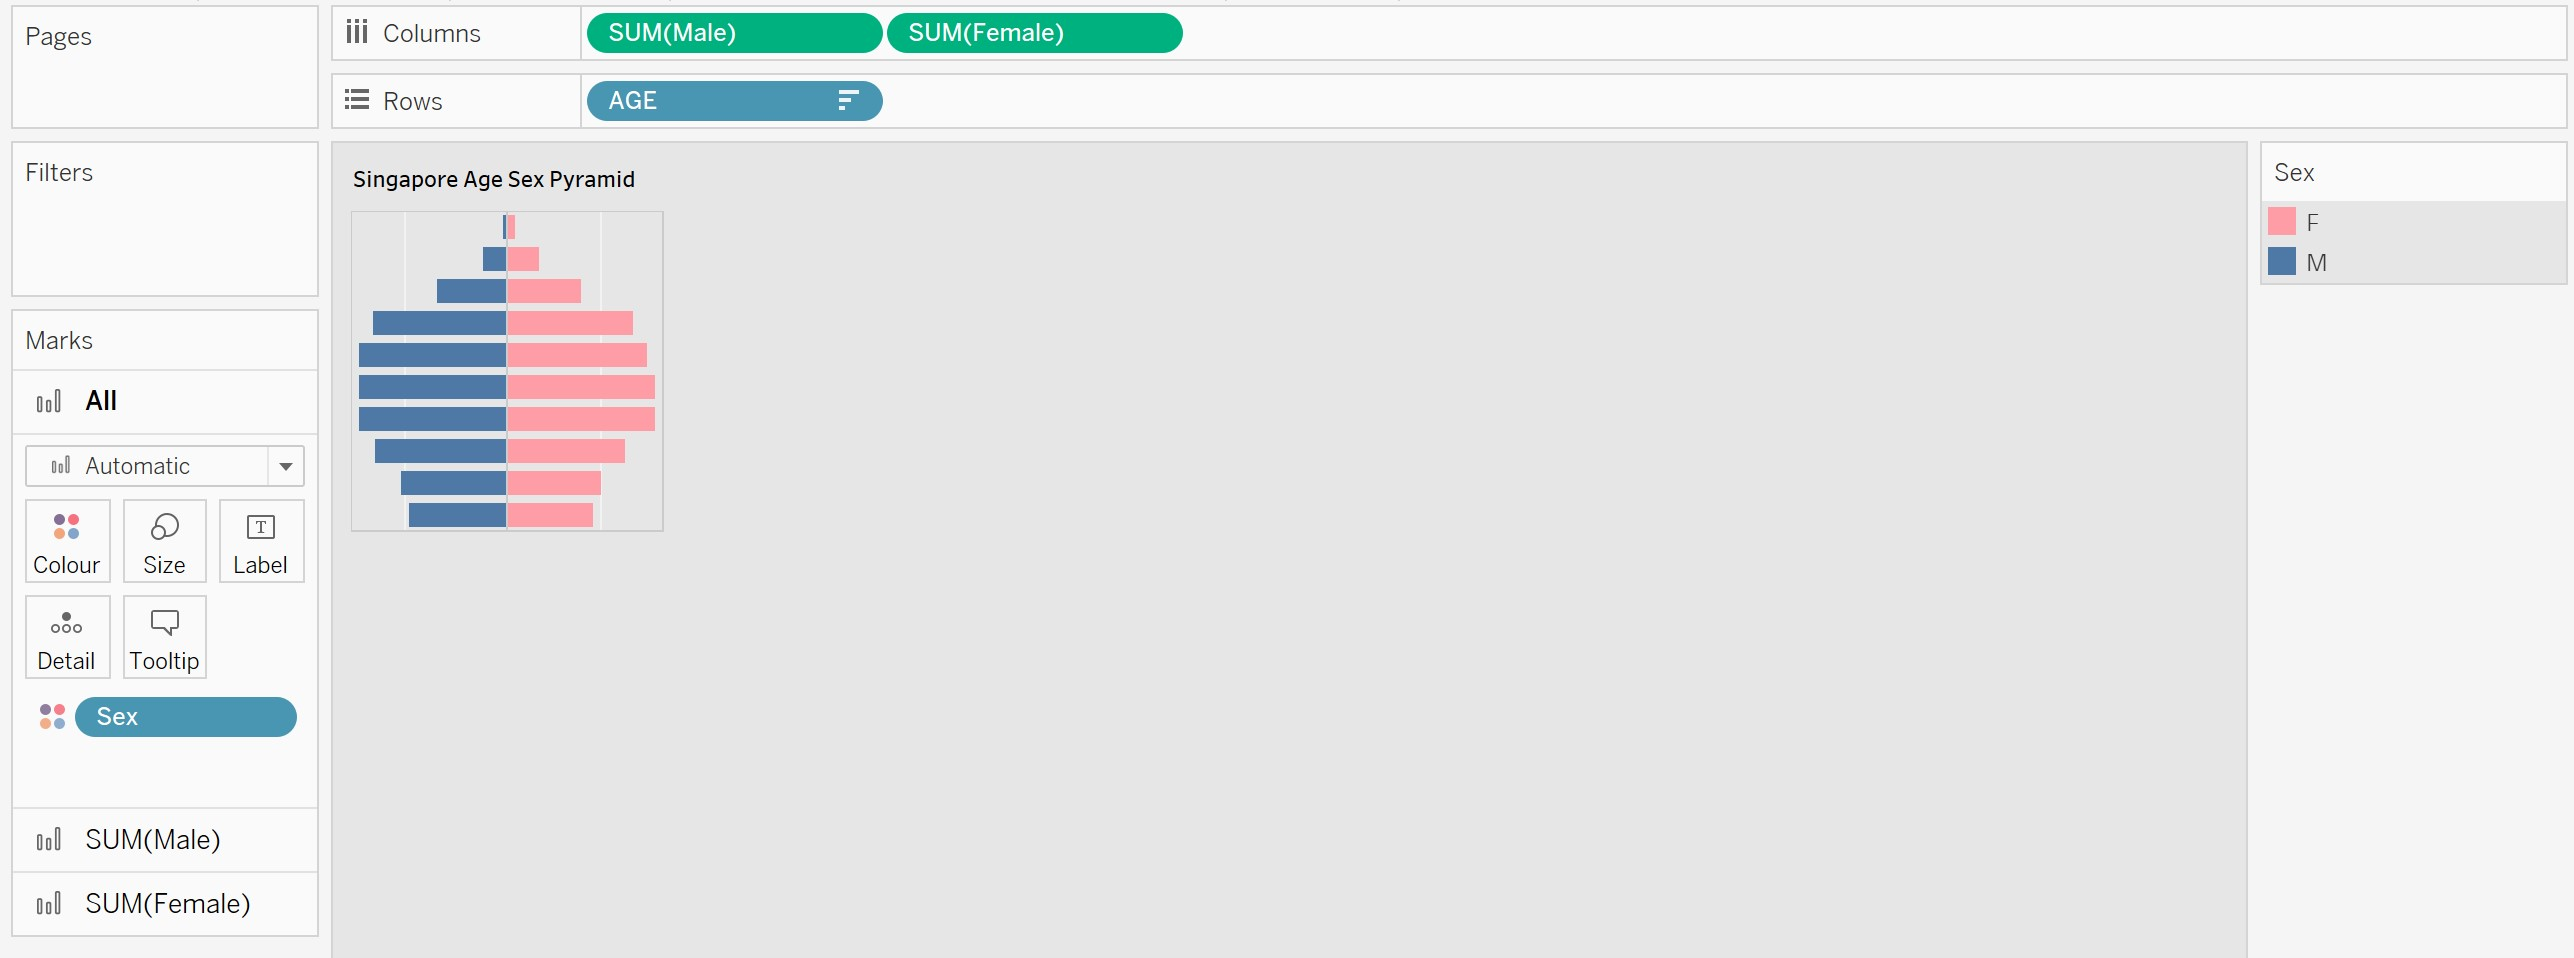
\includegraphics{images/Singapore pyramid.jpg} \\
21 & Create a table showing the Old Age Support Ratio of each PA. &
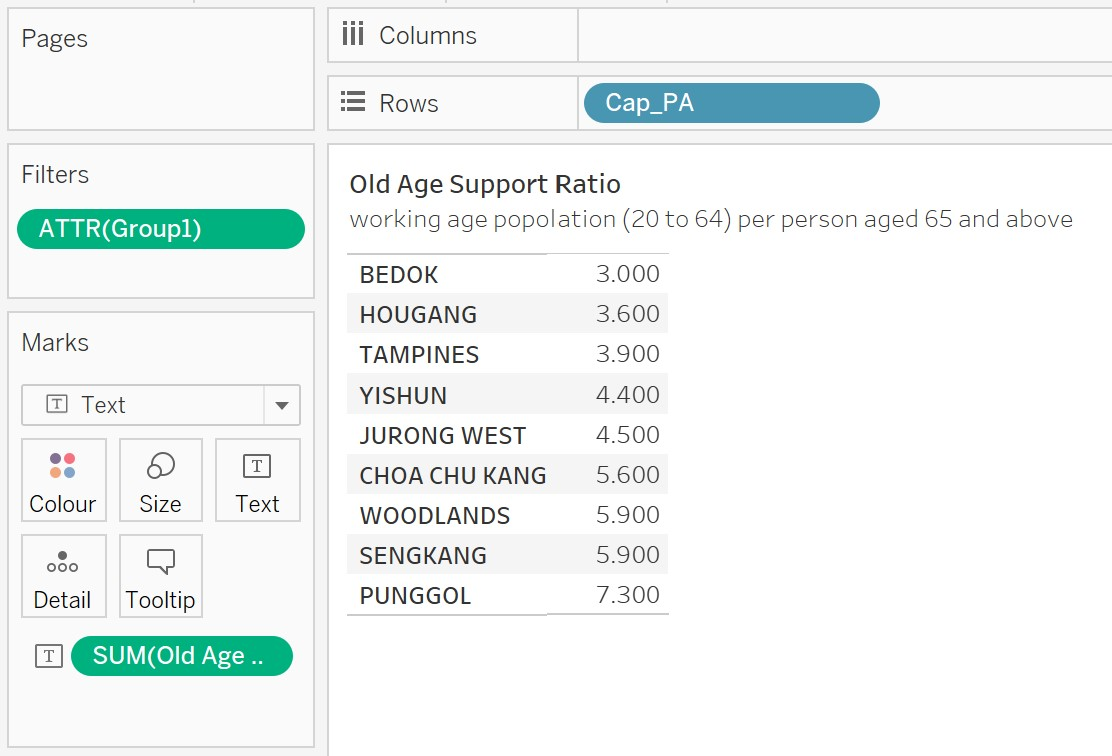
\includegraphics{images/old age support ratio.jpg} \\
22 & Create a new dashboard and drop the worksheets to specific
locations and adjust the width and height of each region.

Add Note, data source and update date. &
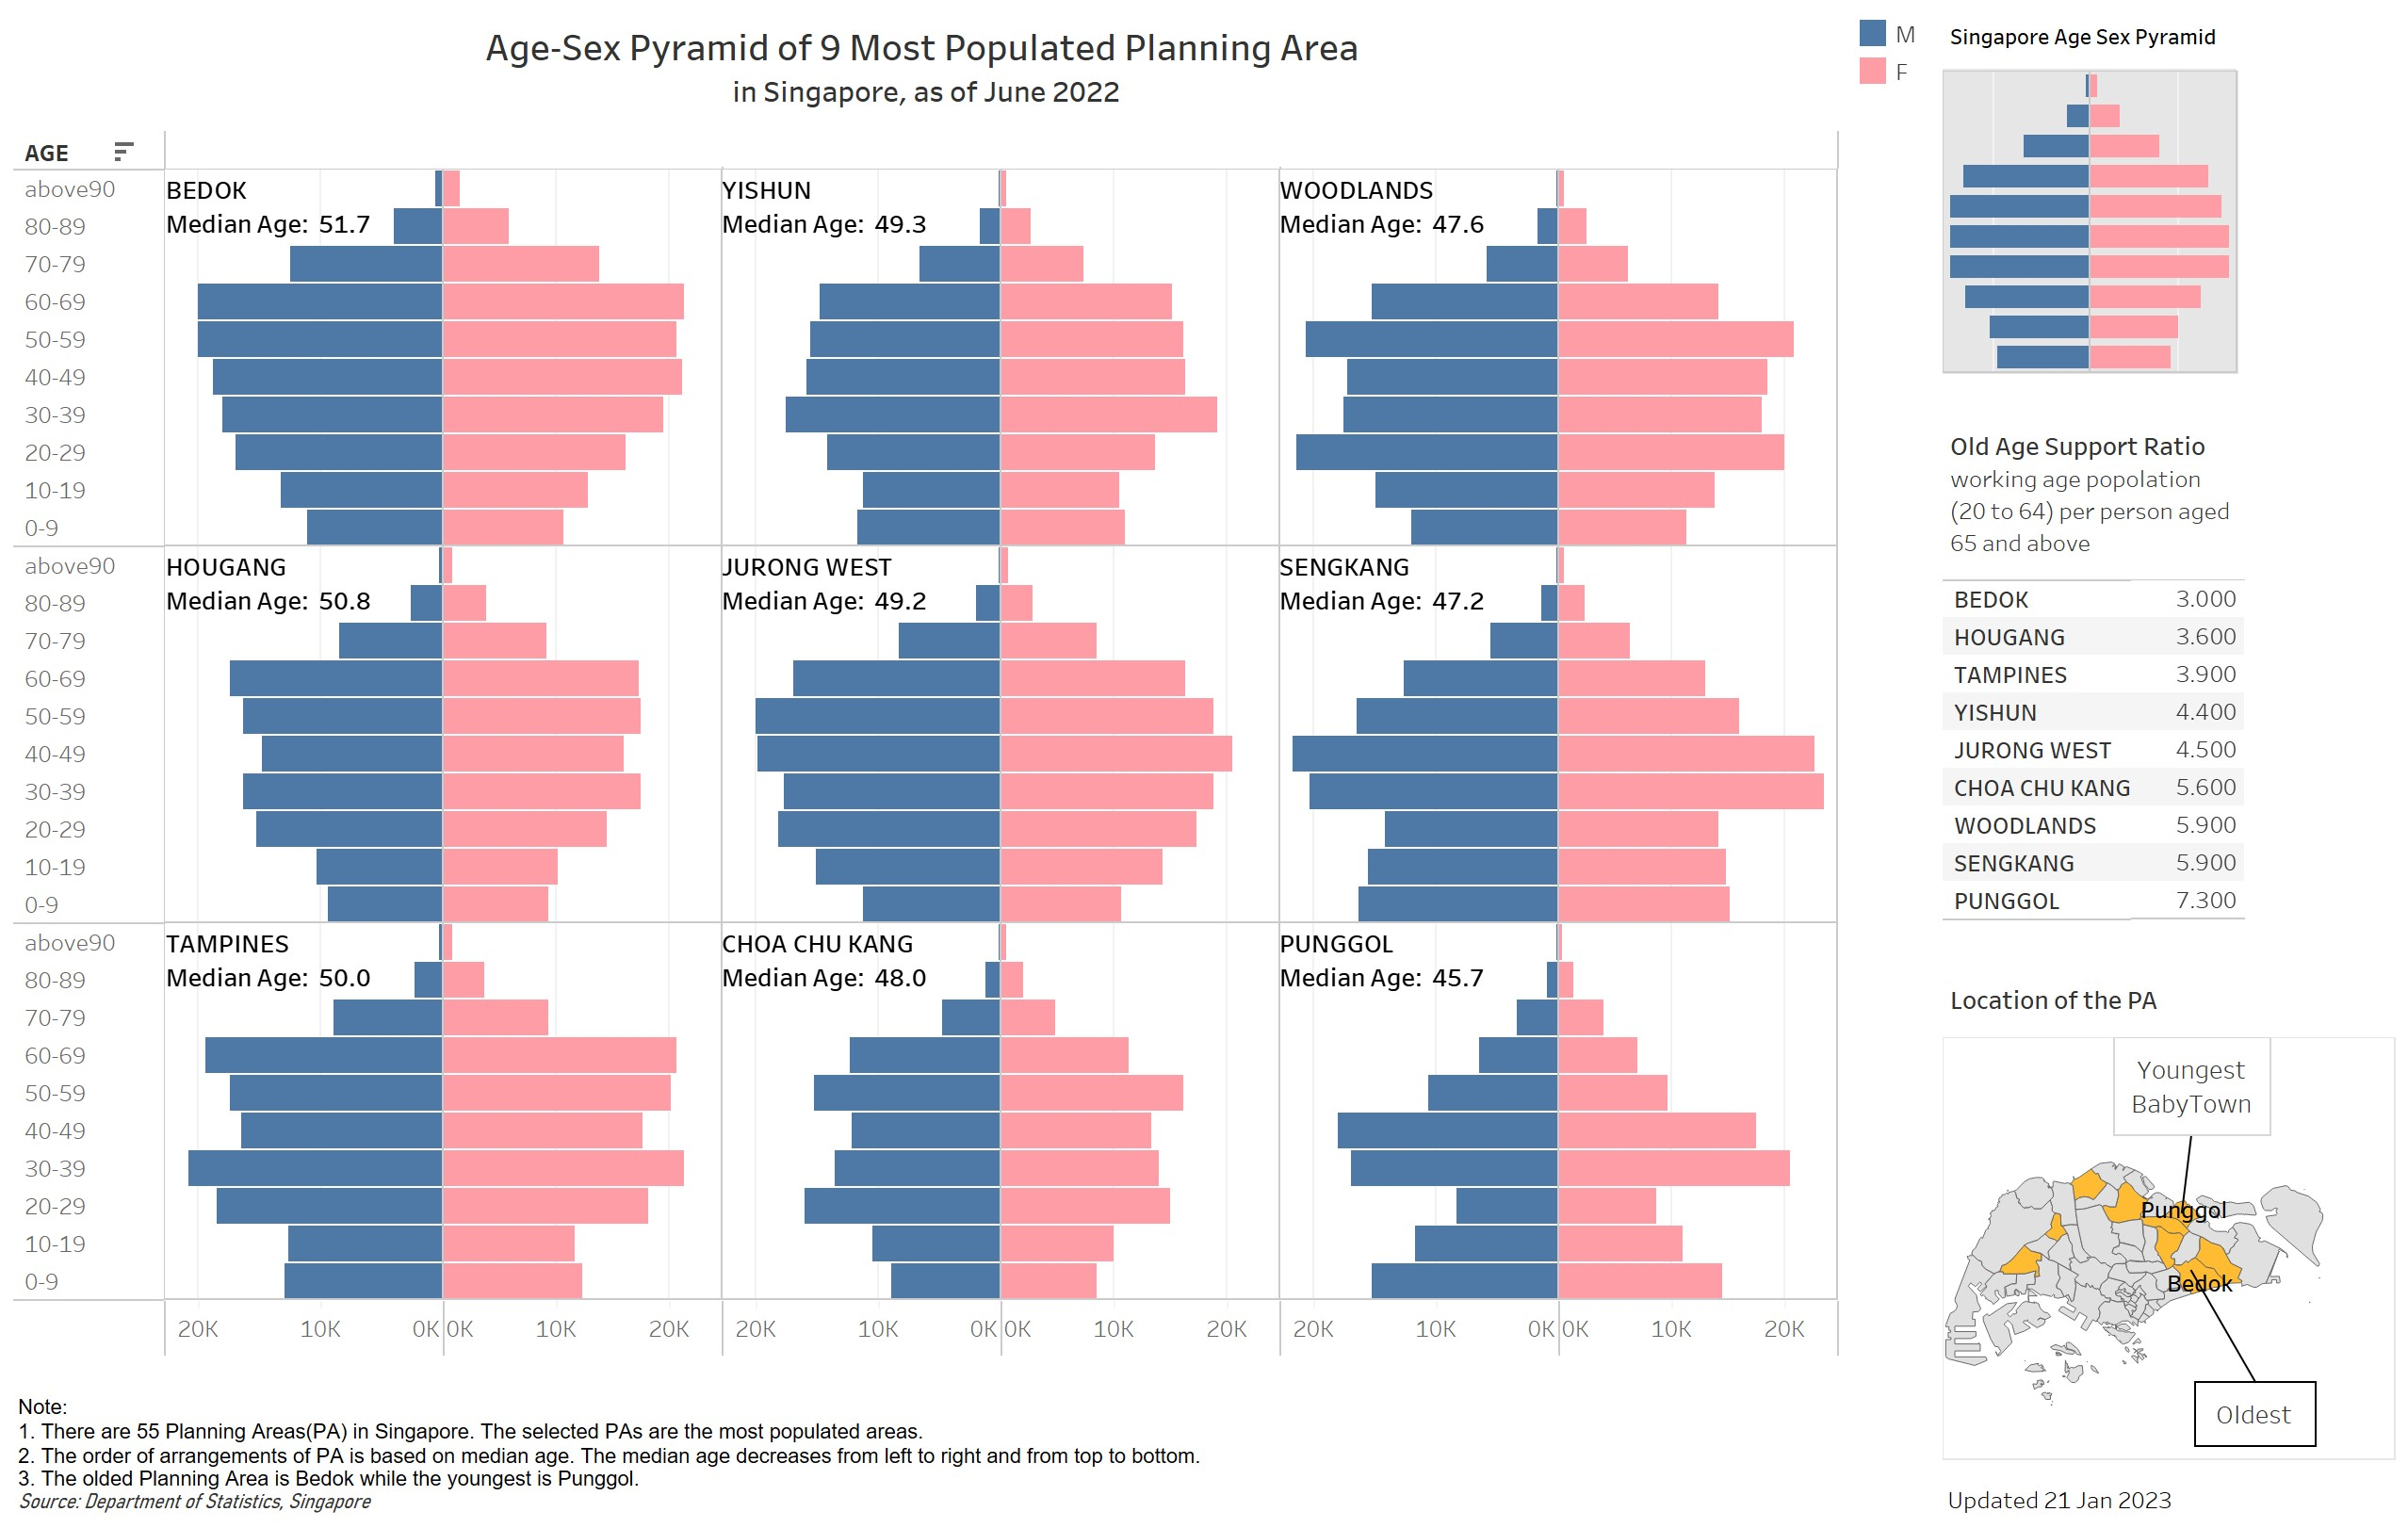
\includegraphics{images/vis-03.jpg} \\
23 & Publish the dashboard. Note that we need to choose to Extract Data,
instead of using Live Data. &
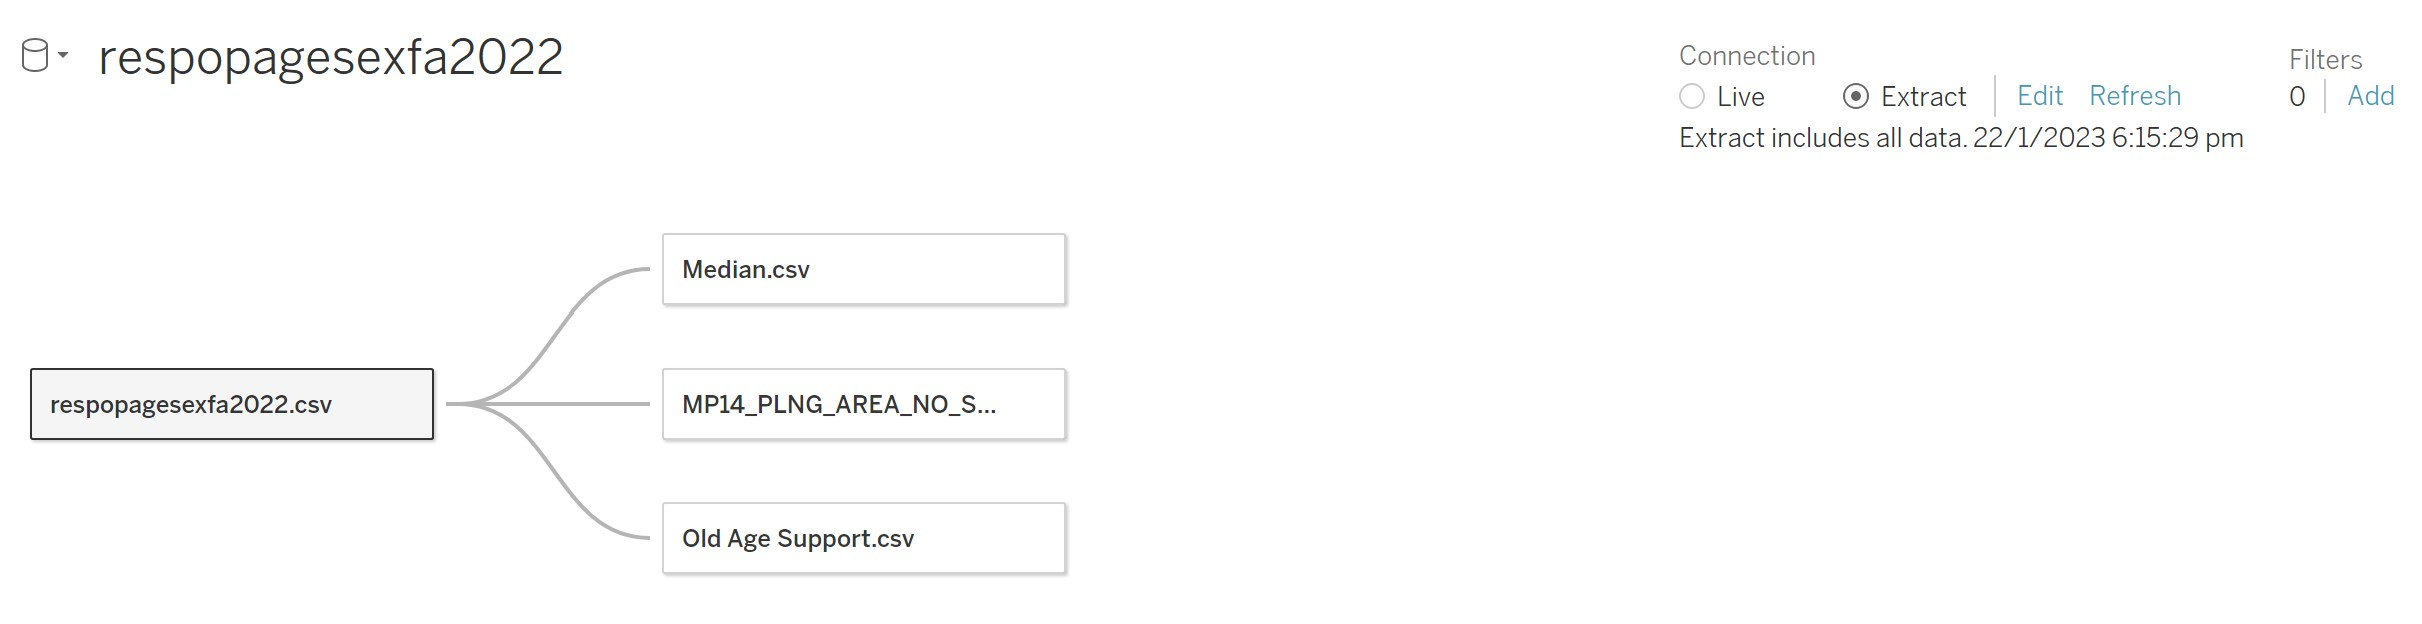
\includegraphics{images/extract data.jpg} \\
\bottomrule()
\end{longtable}

\end{figure*}

\emph{I appreciate you taking the time to read this article and paying
attention to it.}



\end{document}
